% \iffalse meta-comment
%
% Copyright (C) \the\year by Liu Benyuan <liubenyuan@gmail.com>
% This file may be distributed and/or modified under the
% conditions of the LaTeX Project Public License, either
% version 1.2 of this license or (at your option) any later
% version. The latest version of this license is in:
%
% http://www.latex-project.org/lppl.txt
%
% and version 1.2 or later is part of all distributions of
% LaTeX version 1999/12/01 or later.
%
% \fi
% 
% \iffalse
% <package>\NeedsTeXFormat{LaTeX2e}[1999/12/01]
% <package>\ProvidesPackage{nudtpaper}
% <package>[2015/05/12 v2.5 By Liu Benyuan <liubenyuan@gmail.com>]
%<*driver>
\ProvidesFile{nudtpaper.dtx}[2015/05/12 v2.5 NUDT]
\documentclass[11pt]{ltxdoc}
\usepackage{nudtx}
\EnableCrossrefs
\CodelineIndex
\RecordChanges
\begin{document}
  \DocInput{\jobname.dtx}
\end{document}
%</driver>
% \fi
% 
% \def\thuthesis{\textsc{Thu}\-\textsc{Thesis}}
% \def\nudtpaper{\textsc{Nudt}\-\textsc{Paper}}
% 
% \CheckSum{1217}
% \CharacterTable
%  {Upper-case    \A\B\C\D\E\F\G\H\I\J\K\L\M\N\O\P\Q\R\S\T\U\V\W\X\Y\Z
%   Lower-case    \a\b\c\d\e\f\g\h\i\j\k\l\m\n\o\p\q\r\s\t\u\v\w\x\y\z
%   Digits        \0\1\2\3\4\5\6\7\8\9
%   Exclamation   \!     Double quote  \"     Hash (number) \#
%   Dollar        \$     Percent       \%     Ampersand     \&
%   Acute accent  \'     Left paren    \(     Right paren   \)
%   Asterisk      \*     Plus          \+     Comma         \,
%   Minus         \-     Point         \.     Solidus       \/
%   Colon         \:     Semicolon     \;     Less than     \<
%   Equals        \=     Greater than  \>     Question mark \?
%   Commercial at \@     Left bracket  \[     Backslash     \\
%   Right bracket \]     Circumflex    \^     Underscore    \_
%   Grave accent  \`     Left brace    \{     Vertical bar  \|
%   Right brace   \}     Tilde         \~}
%
% \changes{v0.99}{2009/08/12}{Initial Release}
%
% \GetFileInfo{\jobname.dtx}
% 
% \DoNotIndex{\begin,\end,\begingroup,\endgroup}
% \DoNotIndex{\ifx,\ifdim,\ifnum,\ifcase,\else,\or,\fi}
% \DoNotIndex{\let,\def,\xdef,\newcommand,\renewcommand}
% \DoNotIndex{\expandafter,\csname,\endcsname,\relax,\protect}
% \DoNotIndex{\Huge,\huge,\LARGE,\Large,\large,\normalsize}
% \DoNotIndex{\small,\footnotesize,\scriptsize,\tiny}
% \DoNotIndex{\normalfont,\bfseries,\slshape,\interlinepenalty}
% \DoNotIndex{\hfil,\par,\hskip,\vskip,\vspace,\quad}
% \DoNotIndex{\centering,\raggedright}
% \DoNotIndex{\c@secnumdepth,\@startsection,\@setfontsize}
% \DoNotIndex{\ ,\@plus,\@minus,\p@,\z@,\@m,\@M,\@ne,\m@ne}
% \DoNotIndex{\@@par,\DeclareOperation,\RequirePackage,\LoadClass}
% \DoNotIndex{\AtBeginDocument,\AtEndDocument}
%
% \IndexPrologue{\section*{索引}%
%    \addcontentsline{toc}{section}{索~~~~引}}
% \GlossaryPrologue{\section*{修改记录}%
%    \addcontentsline{toc}{section}{修改记录}}
%
% \renewcommand{\abstractname}{摘~~要}
% \renewcommand{\contentsname}{目~~录}
%
% \title{\textsc{NUDTpaper:}\,\,NUDT研究生学位论文\LaTeX{}模板使用手册\thanks{NUDT \LaTeX{} Thesis Template}}
% \author{刘本源 \\ \texttt{Liubenyuan@gmail.com}}
% \date{\fileversion\ (\filedate)}
%
% \maketitle
% \thispagestyle{empty}
%
% \begin{abstract}
% 本模板旨在提供规范的国防科学技术大学\LaTeX{}写作模板环境,
% 现支持硕士/博士学位论文格式,可以自动生成盲评、制作A3封面。
% \end{abstract}
%
% \vspace{2cm}
% \def\abstractname{免责声明}
% \begin{abstract}\noindent
% \begin{enumerate}
% \item 本模板的发布遵守 \LaTeX{} Project Public License,使用前请认真阅读协议内容
% \item 本模板创立参照官方严格的论文写作手册,并同时参照硕士/博士学位论文\textbf{doc}文档对比修改
% \item 国防科学技术大学对论文写作提供写作指南与官方\textbf{doc}模板,
% 同时提供官方的\LaTeX{}模板,本模板的出发点是方便大家使用专业的高效的论文书写工具,
% 其有点在于注重排版质量、命令规范、使用方便、更新及时,符合论文撰写说明。
% 但任何由于使用本模板而引起的论文格式审查问题均与本模板作者无关。
% \item 任何个人或组织均可以本模板为基础进行修改、扩展,生成新的专用模板,但请严格遵
% 守\LaTeX{} Project Public License 协议
% \item 欢迎提出修改意见
% \end{enumerate}
% \end{abstract}
%
% \clearpage
% \tableofcontents
%
% \clearpage
% \pagenumbering{arabic}
% \pagestyle{mainpage}
%
% \section{快速上手}
% \begin{description}
% \item[安装\TeX] 下载最新的\TeX{}live或者C\TeX{}并安装
% \item[字体] 用户需要具备\verb|simsun.ttf|, \verb|simhei.ttf|, \verb|simkai.ttf|,
% \verb|STZHONGS.TTF|, 上述字体都是windows自带的; 除此之外,在网上搜索(或者C\TeX{}
% 论坛)``Adobe Opentype 中文字体'',一搜一大把,确保下载下来Adobe的四款OTF字体:
% 宋,黑,仿宋,楷体。Linux用户可将上述字体复制到\verb|/usr/share/fonts/TTF|下。
% 最新更新:用户可以考虑使用方正字体生成更为漂亮(颜色深均匀)的论文排版。
% 这三个选项分别为\verb|ttf|、\verb|otf|和\verb|fz|。
% \item[试一试] 解压缩下载的模板,双击makepdf.bat(祈祷一下),如果生成了
% \verb|thesis.pdf|$\rightarrow$
% \item[那么我的那些常用的包都在么?] 你会想我的{\bf Trans}论文可以无缝
% 的复制过来么? 对于这一点,你可以修改\verb|mynudt.sty|来实现。但是{\hei 注意},大部分包
% 都在模板中了,而且{\hei 切记切记},不要擅自改动字体等版面设计,我们继续看$\rightarrow$
% \item[咦,数学公式不是很美观呀] 笔者{\hei 强烈}建议用户使用{\bf mtpro2}宏包的,怎么使用,
% 又有哪些好处,参见bookzh.sty吧!不会错的。好了,我们专注于内容本身吧$\rightarrow$
% \item[开始写了] 所有文件均采用UTF8编码,因此要保证你的\TeX{}编辑器
% (winedt, texworks, texmaker, vim, 记事本($\cdots{}$)等)支持这种编码,
% (经过一番搜索设置后)打开\verb|thesis.tex|,如果看到的是中文$\rightarrow$
% \item[漫长的写作] 手边准备着\LaTeX{}的常用帮助文档(数学,图表,引用等),
% 结合你喜欢的文献管理软件(JabRef等), 漫长的\texttt{编辑,编译,修改,编辑,
% 编译$\cdots$}过程之后,突然有一天发现你写完了$\rightarrow$
% \item[校订] 经过老师师兄师弟师妹齐心协力校正之后,你所做的只是:
% \texttt{生成明评论文,制作明评封面,生成盲评论文,制作盲评封面},
% 装订,上交$\rightarrow$
% \end{description}
% {\color{magenta} Done!}
%
% \section{模板介绍}
%
% \textsc{NUDTpaper} 旨在帮助并且推广\LaTeX{}在国防科技大学论文中的应用,
% 本文将尽可能帮助用户掌握\textsc{NUDTpaper}的安装方法,
% 如果仍旧有不清晰的地方可以参考样例文件或者
% 给作者邮件\footnote{liubenyuan@gmail.com},感兴趣的同学可以帮忙维护模板,
% 这个模板首先符合官方的设计要求,希望同学们在使用后能够提出你们的修改意见。
% 该模板很大程度上参考了6院黄老师sofoot的国防科大博士论文模板,
% 哈工大的\LaTeX{}模板以及清华的Thuthesis
% \footnote{主页:\url{http://thuthesis.sourceforge.net}},
% 有很多使用的帮助、\verb|.cls|中的命令以及版面设置均来自Thuthesis和sofoot的模板,
% 对此的引用表示感谢。
%
% {\color{blue}\fs 模板的作用在于减轻论文写作过程中格式调整的时间,
% 其前提就是遵守模板的用法,不提倡手动更改格式,不建议正文中使用
% 手动调节版面的命令,尤其禁止修改行距和使用\verb|\normalsize|,
% 否则即使使用了\textsc{NUDTpaper}也难以保证输出的论文符合学校规范。}
%
% \section{安装}
% \label{sec:install}
%
% \subsection{下载}
% \textsc{NUDTpaper} 主页:\url{http://nudtpaper.googlecode.com}。
% 模板的更新信息发布在\href{http://bbs.ctex.org}{Ctex论坛}。
% \nudtpaper{}的开发版本同样可以在\textsc{gitorious}上获得。
%
% \subsection{模板的组成部分}
% 下表列出了 \nudtpaper{} 的主要文件及其功能介绍,学习模板的最好办法
% 就是参考thesis.pdf!
% \begin{center}
% \begin{longtable}{l|p{8cm}}
% \toprule
% {\hei 文件(夹)} & {\hei 功能描述}\\\midrule
% \endfirsthead
% \toprule
% {\hei 文件(夹)} & {\hei 功能描述}\\\midrule
% \endhead
% \endfoot
% \endlastfoot
% nudtpaper.ins & 模板驱动文件 \\
% nudtpaper.dtx & 模板文档代码的混合文件\\
% nudtpaper.cls & 模板类文件\\
% nudtpaper.cfg & 模板配置文件\\
% thesis.bib & 参考文献样式文件\\
% \hline
% mynudt.sty & 在这里添加你自己的宏包 \\
% thesis.tex & 示例文档主文件\\
% ref/ & 示例文档参考文献目录\\
% data/ & 示例文档章节具体内容\\
% figures/ & 示例文档图片路径\\
% \textbf{nudtpaper.pdf} & 用户手册(本文档)\\
% \textbf{thesis.pdf} & 示例文档 \\
% \bottomrule
% \end{longtable}
% \end{center}
%
% \subsection{\TeX{}系统的选择}
% 有网络环境的用户推荐安装\href{http://www.tug.org/texlive}{\TeX{}live},
% \href{http://miktex.org}{MiKTeX}或者\href{http://www.ctex.org}{C\TeX},
% 对于无网络环境的,主要是针对教研室用户,推荐{\TeX{}live}或者C\TeX{}完整版,安装
% 过程很简单,一路下一步即可,但是需要\textbf{注意:}
%
% \begin{description}
% \item[字体] TTF选项默认调用Windows系统字体,其中楷体、仿宋需要安装Office;OTF选项需要
% Adobe的商业字体(可以使你的论文更加漂亮!),这些中文字体(宋,黑,仿宋,楷体)可以从
% \href{http://dl.getdropbox.com/u/857066/adobe_chinese_otf.7z}{这里下载},
% 如果上述链接不能使用,请搜索\textsc{Adobe Opentype 中文字体}自行下载。
% 英文字体使用Windows自带。起始更推荐几款Times(Arial)类似的OTF英文字体,可以使用
% 更多排版、段落的字体特性。
% \item[粗宋] 模板中在需要宋体加黑的地方需要使用\textbf{华文中宋}, 即STZHONGS.TTF。
% \item[xeCJK] 无网络环境中,C\TeX{}完整版和\TeX{}live最新版都包括了需要的xeCJK版本。
% \end{description}
%
% \subsection{使用模板}
% \label{sec:install-cls}
% {\hei 注:默认的发行版本已经包含了可以使用的模板环境,
% 包括编译好的cls以及论文样例源文件,
% 想快速上手的话,可以直接参看\verb|thesis.tex|,进行修改。
% 写作的过程就是将你的论文的内容放到\verb|data|文件夹中,
% 图片放到\verb|figures|文件夹中,用\textsc{jabref}修改\verb|thesis.bib|即可。}
%
% 当用户需要编译生成自己的PDF版论文时,需要依次输入:(注意了,如果不是使用nomencl,
% 则无需使用第二个命令)
% \begin{shell}
% $ xelatex thesis
% $ # makeindex -s nomencl.ist -o thesis.nls thesis.nlo
% $ bibtex thesis
% $ bibtex thesis
% $ xelatex thesis
% $ xelatex thesis
% \end{shell}
%
% 而为了简化用户使用,模板中提供了快捷脚本文件:
% \begin{shell}
% # 下面命令可以直接生成thesis.pdf,你可能只需要这步
% C:\> makepdf.bat
% # linux用户可以直接使用makefile
% $ make pdf
% \end{shell}
% 现在,就要进入激动人心的写作过程了。
%
% \section{使用说明}
% \label{sec:how-to-use}
% 首先,一篇论文(电子信息工程专业为例),主要的构成就是
% 封面导言,正文,表格,图片,公式,
% 交叉引用及文献索引这五部分,下面将分别详细讲解。
%
% \label{sec:howtoask}
% 在开始之前,先问自己几个问题:
% \begin{compactenum}
% \item 我是不是已经掌握了 \LaTeX{} 基础知识?
% \item 我是不是认真地阅读了模板文档?
% \item 周围有没有同学可以帮我?
% \end{compactenum}
% 更推荐用户去阅读示例文档的源代码,改写会给你一个快速的开始。
%
% \subsection{示例文件}
% \label{sec:example}
% 该示例文件是顶层的文件,包括论文属性设置、章节的安排、参考文献附录等。
% 细节用户可以参考\verb|thesis.tex|和\verb|data/|文件夹。
%
% \subsubsection{模板选项}
%
% 论文的第一句话是调用模板:
% \changes{v2.0}{2010/11/10}{增加盲评的说明}
%
%    \begin{macrocode}
%<thesis>%1. 规范硕士导言
%<thesis>% \documentclass[master,ttf]{nudtpaper}
%<thesis>%2. 规范博士导言
%<thesis>% \documentclass[doctor,twoside,ttf]{nudtpaper}
%<thesis>%3. 建议使用OTF字体获得较好的页面显示效果
%<thesis>%   OTF字体从网上获得,各个系统名称统一。
%<thesis>%   如果你下载的是最新的(1201)OTF英文字体,建议修改nudtpaper.cls,使用
%<thesis>%   Times New Roman PS Std
%<thesis>% \documentclass[doctor,twoside,otf]{nudtpaper}
%<thesis>%   另外,新版的论文模板提供了方正字体选项FZ,效果也不错哦
%<thesis>% \documentclass[doctor,twoside,fz]{nudtpaper}
%<thesis>%4. 如果想生成盲评,传递anon即可,仍需修改个人成果部分
%<thesis>% \documentclass[master,otf,anon]{nudtpaper}
%<thesis>%
%    \end{macrocode}
%    \begin{macrocode}
%<*thesis>
\documentclass[master,otf]{nudtpaper}
\usepackage{mynudt}

%</thesis>
%    \end{macrocode}
%
% 模板的参数设置(开关)描述见:
%
%\begin{description}
%\item[master,doctor]
% 硕士论文用master,博士论文就用doctor
%\item[twoside]
% 指定论文为单面打印还是双面打印,当使用\verb|twoside|选项之后,
% 论文会将章节开在奇数页右手边,默认为\verb|openany|单面打印。
%\item[ttf,otf]
% 决定使用何种字体,TTF默认使用Windows自带的字体,而OTF则使用Adobe的字体(需要下载),
% TTF字体的优势是满足学校论文对于字体的要求,缺点是制作出来的PDF文件在浏览时可能发虚,
% 而OTF字体屏幕显示饱满,而且字体有很多选项可以方便\XeTeX{}排版。推荐使用\textbf{otf}
% 选项。不论何种选项,都需要安装宋体中宋(STZHONGSONG)字体(Windows自带)。
%\item[anon]
% 是否为盲评版本,如需盲评,请加上anon。
%\end{description}
%
% 如果需要使用自己定义的命令、宏包,请放于\verb|mynudt.sty|中。
% 事实上,该文件中已经添加了很多有用的宏包和命令,你可以参照修改。
% 这些之所以没有放到模板中,一则为了简洁,二则赋予用户在格式之外更多的自由。
% 里面的宏包有:代码高亮、算法环境、向量命令等,请仔细查看。
%
% 样例文件默认的是硕士论文(master),OTF字体(otf)。
%
% \subsubsection{封面导言}
% 官方模板中设计论文题目、作者等信息可以跟填空一样完成:
%
% \begin{description}
% \item[论文封头]
% 主要有四部分内容,中图分类号,学号,论文密级和UDC。
% 密级分为:\textbf{秘密} 或者 \textbf{公开}。
%    \begin{macrocode}
%<*thesis>
\classification{TP957}
\serialno{0123456}
\confidentiality{公开}
\UDC{}
%</thesis>
%    \end{macrocode}
%
% \item[论文题目,作者,日期]
% 分别包括中文和英文两部分,由于论文题目可能超过1行,
% 我们提供额外的一个命令\verb|\displaytitle|用来在
% 授权书中填入(限定为)单行的题目; 中文日期需要中文输入大写,英文日期为月年,
% 在论文最终完成后,请\textbf{手动}设定日期。
% \changes{v2.5}{2015/05/11}{修改英文作者和导师的格式,姓大写}
% \changes{v2.5}{2015/05/11}{英文导师前缀为Prof.}
%
%    \begin{macrocode}
%<*thesis>
\title{国防科大学位论文\LaTeX{}模板\\
使用手册}
\displaytitle{国防科学技术大学学位论文\LaTeX{}模板}
\author{张三}
\zhdate{\zhtoday}
\entitle{How to Use the \LaTeX{} Document Class for NUDT Dissertations}
\enauthor{ZHANG San}
\endate{\entoday}
%</thesis>
%    \end{macrocode}
%
% \item[论文分类及其他]
% 主要是作者的学科类别,研究方向,导师信息等。
% 每一项都包括中英文信息:
%
%    \begin{macrocode}
%<*thesis>
\subject{通信与信息工程}
\ensubject{Information and Communication Engineering}
\researchfield{自动目标识别与模糊工程}
\supervisor{李四\quad{}教授}
\cosupervisor{王五\quad{}副教授} % 没有就空着
\ensupervisor{Prof. LI Si}
\encosupervisor{}
\papertype{工学}
\enpapertype{Engineering}
%</thesis>
%    \end{macrocode}
%
% \item[中英文摘要]
% 论文中需要写中文以及英文摘要,页码为小写罗马字母,关键字为黑体,
% 英文关键字为\verb|Arial|,
% 模板中定义了相关环境\verb|\cabstract|以及\verb|\eabstract|来书写摘要,
% 以及\verb|\ckeywords|以及\verb|\ekeywords|来写关键字。
% 建议用户将摘要单独放在在\verb|abstract.tex|文件中,
% 在正文中\verb|\begin{cabstract}
近年来,随着无人作战系统(Unmanned Combat System,UCS)在伊拉克、阿富汗等几场局部战争的广泛使用,展现了无人作战系统的巨大军事价值。作为无人作战系统中的重要组成,无人机所承担的侦察、监视、通信中继、战场评估、攻击引导等任务也日益增多。为扩大无人机的工作半径,提升作战效能,无人机在舰船上回收的需求更加迫切。虽然无人机在地面起飞、降落或回收已经成为常态,但上述过程中的引导方式主要依赖卫星定位导航系统(Global Navigation Satellite System,GNSS)。在未来“反介入/区域拒止(A2/AD)”的战场环境下,仅仅依赖卫星导航系统无法满足无人机在舰船的降落需求。本文主要针对上述研究背景展开工作,主要完成工作和创新点如下:

(1)提出了一种地基/舰基通用的多传感器无人机回收引导系统。该系统主要有两个独立引导单元组成,每个引导单元配备一个二自由度转台和可见光相机、红外相机等传感器。两个独立引导单元的排布可以根据目标无人机的大小和检测距离进行优化配置。本文针对该系统独立分布在跑道两侧的特点,通过对目标位置解算理论推导、误差分析和实验验证,证明了在无人机降落过程中,使用上述两种引导系统的可行性。

(2)设计并实现无人机降落过程中实时目标跟踪和位置解算算法。针对引导无人机降落过程中,无人机目标尺度快速变化和姿态未知的问题,通过改进基于形态学滤波的图像预处理方法,TLD目标跟踪框架和基于主动轮廓的目标位置修正方法,结合转台运动位置和无人机运动的估计,能够准确解算出无人机在降落过程中相对于舰船的位置信息,满足无人机引导和控制系统的需要。

(3)设计并实现基于非线性模型预测控制(NMPC)和总能量控制(TESC)的无人机着舰控制系统。由于无人机机载设备运算能力的约束,本文设计了内环控制器和外环控制器来实现无人机的自主降落。其中内环控制器主要由PI和PID控制器组成,主要完成对无人机姿态的控制;外环控制器主要由非线性模型预测控制器(NMPC)和总能量控制器(TESC)组成,针对基于Dubins Path生成的降落曲线进行跟踪。

(4)设计并实现无人机舰载着舰系统仿真环境并进行户外实验验证。本文基于机器人操作系统(Robot Operation System,ROS)和Gazebo仿真环境构建了无人机舰载着陆软件在回路仿真系统(SITL)和硬件在回路仿真系统(HIL)。该仿真环境能够满足上述算法的验证需求。通过二自由度转台与多传感器的组合配置,实现在地面机场和水面环境对小型和中型固定翼无人机的引导和自主降落。

上述理论和算法成果分别发表在2012年和2013年的IEEE/RSJ智能机器人与系统国际会议(IROS)会议,得到了领域内同行的认可。基于上述算法的实际飞行测试分别在江西吉安机场和湖南长沙湘江水域进行,验证了基于多传感器的地基引导系统和舰基引导系统的可行性和可靠性。

\end{cabstract}
\ckeywords{无人机;自主着舰;多传感器引导与控制;}

\begin{eabstract}
 In recent years, with the unmanned combat system(UCS) in Iraq, Afghanistan and several other local wars of widespread use, unmanned combat system is showing the great military value. As an important component of unmanned combat system, unmanned aerial vehicles(UAVs) are increasingly assigned with reconnaissance, surveillance, communication relay, battlefield evaluation and attack guidance. In order to expand the operating radius of UAV, improve combat effectiveness, the demand of autonomous landing on a destroyer or carrier is continuing to grow. Although UAVs take off and landing on the standard airport is quite common, navigation in the above maneuvers relies mainly on the Global Navigation Satellite System (GNSS). In the future A2 / AD battlefield environment, the satellite navigation system alone can not meet the UAVs' landing demand. This paper aims at the above research background, the main work and innovation are as follows:
 
(1) A ground / ship-based multi-sensor unmanned aerial vehicle (UAV) recovery and guidance system is proposed. The system consists of two independent guidance units, each with a two degrees of freedom PTU(Pan/Tilt Unit) and visible light camera, infrared camera or other sensors. The configuration of the two independent guidance units can be optimally setup according to the size of the UAV and the proposed detection distance. In this thesis, the feasibility of using the above two guidance systems in the process of UAV landing is proved by the theory of target position solution, error analysis and experimental verification, which is based on the characteristics of the system distributed on both sides of the runway independently.

(2) Design and implement the real-time target tracking and location algorithm in UAV landing process. Aiming at the problem of traking the UAV, size rapidly changing from tiny to large scale, the method of image preprocessing based on morphological filtering, TLD target tracking framework and target position updating based on active contour are improved. During the landing process, the Motion position and unmanned aerial vehicle motion estimation, can accurately calculate the position of UAV relative to the ship's position 

(3) Design and implementation of the non-linear model predictive control (NMPC) and total energy control (TESC) of the UAV landing control system. Due to the computation constraints of UAV on-board equipment, the inner-loop controller and the outer-loop controller are designed to realize the autonomous landing. The inner loop controller is mainly composed of PI controller and PID controller. The outer loop controller mainly consists of nonlinear model predictive controller (NMPC) and total energy controller (TESC) in order to tracking the landing curve which generated by Dubins Path algorithms.

(4) Design and implement the simulation system and experimental verification system for UAV shipboard landing problem. Based on the Robot Operation System (ROS) and Gazebo simulation environment, a software in the loop simulation system (SITL) and hardware in the loop simulation system (HIL) is constructed. The simulation environment can meet the verification requirements of the above algorithms. By selecting PTUs and reltaed sensors, autonomous guidance and landing of the UAV can be achieved at ground and airfields.

The above theoretical and algorithmic results were published in the 2012 IEEE / RSJ Intelligent Robot and Systems International Conference (IROS) meeting in 2012 and were recognized by peers in the field. The actual flight tests based on the above algorithms were carried out in Ji'an Airport of Jiangxi Province and Xiangjiang River of Changsha, Hunan Province, respectively. The feasibility and reliability of the foundation guidance system and ship-based guidance system based on multi-sensor were verified.
 
 
\end{eabstract}
\ekeywords{UAV; Autonomous Landing; Multi-sensor Guidance and Control}

|即可。其格式为:
%
% \begin{example}
% \begin{cabstract}
% 中文摘要
% \end{cabstract}
% \ckeywords{关键字}
%
% \begin{eabstract}
% Abstract
% \end{eabstract}
% \ekeywords{Key}
% \end{example}
% \end{description}
%
% \subsubsection{框架构成}
%
% 在定义完论文元素之后,就可以开始写论文正文了。用\LaTeX{}写论文的文件目录构成
% 可以很随意,模板中将图形文件单独放到一个目录中\verb|figure|中,论文正文各个
% 章节置于\verb|data|中;当然也以以\verb|chapter|为目录。
%\changes{v2.2}{2011/05/27}{使用nomencl包管理符号列表}
%\changes{v2.2}{2011/07/08}{默认使用nomencl管理参考文献}
%\changes{v2.2}{2011/09/10}{回复原先使用的denotation方式添加符号列表}
% 
% 如果使用nomencl制作符号列表,在文档开始前要加入\verb|\makenomenclature|命令
% 默认还是使用denotation的方式。nomencl可以参考第二章相关章节,而denote方式
% 请参考\verb|data/denotation.tex|文件(简单的列表环境)。
% 
%<thesis>% 加入makenomenclature命令可用nomencl制作符号列表。
%
%    \begin{macrocode}
%<*thesis> 

\begin{document}
\graphicspath{{figures/}}
%</thesis>
%    \end{macrocode}
% 制作完封面后就是正文四大部分了,分别为:
%
% \begin{compactenum}
% \item frontmatter: 生成目录,图目录,表目录
% \item midmatter: 摘要,符号列表
% \item mainmatter: 正文,致谢,文献,成果
% \item backmatter: 附录
% \end{compactenum}
%
%<thesis>% 制作封面,生成目录,插入摘要,插入符号列表 \\
%<thesis>% 默认符号列表使用denotation.tex,如果要使用nomencl \\
%<thesis>% 需要注释掉denotation,并取消下面两个命令的注释。 \\
%<thesis>% cleardoublepage% \\
%<thesis>% printnomenclature% \\
%
%    \begin{macrocode}
%<*thesis>
\maketitle
\frontmatter
\tableofcontents
\listoftables
\listoffigures

\midmatter
\begin{cabstract}
近年来,随着无人作战系统(Unmanned Combat System,UCS)在伊拉克、阿富汗等几场局部战争的广泛使用,展现了无人作战系统的巨大军事价值。作为无人作战系统中的重要组成,无人机所承担的侦察、监视、通信中继、战场评估、攻击引导等任务也日益增多。为扩大无人机的工作半径,提升作战效能,无人机在舰船上回收的需求更加迫切。虽然无人机在地面起飞、降落或回收已经成为常态,但上述过程中的引导方式主要依赖卫星定位导航系统(Global Navigation Satellite System,GNSS)。在未来“反介入/区域拒止(A2/AD)”的战场环境下,仅仅依赖卫星导航系统无法满足无人机在舰船的降落需求。本文主要针对上述研究背景展开工作,主要完成工作和创新点如下:

(1)提出了一种地基/舰基通用的多传感器无人机回收引导系统。该系统主要有两个独立引导单元组成,每个引导单元配备一个二自由度转台和可见光相机、红外相机等传感器。两个独立引导单元的排布可以根据目标无人机的大小和检测距离进行优化配置。本文针对该系统独立分布在跑道两侧的特点,通过对目标位置解算理论推导、误差分析和实验验证,证明了在无人机降落过程中,使用上述两种引导系统的可行性。

(2)设计并实现无人机降落过程中实时目标跟踪和位置解算算法。针对引导无人机降落过程中,无人机目标尺度快速变化和姿态未知的问题,通过改进基于形态学滤波的图像预处理方法,TLD目标跟踪框架和基于主动轮廓的目标位置修正方法,结合转台运动位置和无人机运动的估计,能够准确解算出无人机在降落过程中相对于舰船的位置信息,满足无人机引导和控制系统的需要。

(3)设计并实现基于非线性模型预测控制(NMPC)和总能量控制(TESC)的无人机着舰控制系统。由于无人机机载设备运算能力的约束,本文设计了内环控制器和外环控制器来实现无人机的自主降落。其中内环控制器主要由PI和PID控制器组成,主要完成对无人机姿态的控制;外环控制器主要由非线性模型预测控制器(NMPC)和总能量控制器(TESC)组成,针对基于Dubins Path生成的降落曲线进行跟踪。

(4)设计并实现无人机舰载着舰系统仿真环境并进行户外实验验证。本文基于机器人操作系统(Robot Operation System,ROS)和Gazebo仿真环境构建了无人机舰载着陆软件在回路仿真系统(SITL)和硬件在回路仿真系统(HIL)。该仿真环境能够满足上述算法的验证需求。通过二自由度转台与多传感器的组合配置,实现在地面机场和水面环境对小型和中型固定翼无人机的引导和自主降落。

上述理论和算法成果分别发表在2012年和2013年的IEEE/RSJ智能机器人与系统国际会议(IROS)会议,得到了领域内同行的认可。基于上述算法的实际飞行测试分别在江西吉安机场和湖南长沙湘江水域进行,验证了基于多传感器的地基引导系统和舰基引导系统的可行性和可靠性。

\end{cabstract}
\ckeywords{无人机;自主着舰;多传感器引导与控制;}

\begin{eabstract}
 In recent years, with the unmanned combat system(UCS) in Iraq, Afghanistan and several other local wars of widespread use, unmanned combat system is showing the great military value. As an important component of unmanned combat system, unmanned aerial vehicles(UAVs) are increasingly assigned with reconnaissance, surveillance, communication relay, battlefield evaluation and attack guidance. In order to expand the operating radius of UAV, improve combat effectiveness, the demand of autonomous landing on a destroyer or carrier is continuing to grow. Although UAVs take off and landing on the standard airport is quite common, navigation in the above maneuvers relies mainly on the Global Navigation Satellite System (GNSS). In the future A2 / AD battlefield environment, the satellite navigation system alone can not meet the UAVs' landing demand. This paper aims at the above research background, the main work and innovation are as follows:
 
(1) A ground / ship-based multi-sensor unmanned aerial vehicle (UAV) recovery and guidance system is proposed. The system consists of two independent guidance units, each with a two degrees of freedom PTU(Pan/Tilt Unit) and visible light camera, infrared camera or other sensors. The configuration of the two independent guidance units can be optimally setup according to the size of the UAV and the proposed detection distance. In this thesis, the feasibility of using the above two guidance systems in the process of UAV landing is proved by the theory of target position solution, error analysis and experimental verification, which is based on the characteristics of the system distributed on both sides of the runway independently.

(2) Design and implement the real-time target tracking and location algorithm in UAV landing process. Aiming at the problem of traking the UAV, size rapidly changing from tiny to large scale, the method of image preprocessing based on morphological filtering, TLD target tracking framework and target position updating based on active contour are improved. During the landing process, the Motion position and unmanned aerial vehicle motion estimation, can accurately calculate the position of UAV relative to the ship's position 

(3) Design and implementation of the non-linear model predictive control (NMPC) and total energy control (TESC) of the UAV landing control system. Due to the computation constraints of UAV on-board equipment, the inner-loop controller and the outer-loop controller are designed to realize the autonomous landing. The inner loop controller is mainly composed of PI controller and PID controller. The outer loop controller mainly consists of nonlinear model predictive controller (NMPC) and total energy controller (TESC) in order to tracking the landing curve which generated by Dubins Path algorithms.

(4) Design and implement the simulation system and experimental verification system for UAV shipboard landing problem. Based on the Robot Operation System (ROS) and Gazebo simulation environment, a software in the loop simulation system (SITL) and hardware in the loop simulation system (HIL) is constructed. The simulation environment can meet the verification requirements of the above algorithms. By selecting PTUs and reltaed sensors, autonomous guidance and landing of the UAV can be achieved at ground and airfields.

The above theoretical and algorithmic results were published in the 2012 IEEE / RSJ Intelligent Robot and Systems International Conference (IROS) meeting in 2012 and were recognized by peers in the field. The actual flight tests based on the above algorithms were carried out in Ji'an Airport of Jiangxi Province and Xiangjiang River of Changsha, Hunan Province, respectively. The feasibility and reliability of the foundation guidance system and ship-based guidance system based on multi-sensor were verified.
 
 
\end{eabstract}
\ekeywords{UAV; Autonomous Landing; Multi-sensor Guidance and Control}


\chapter*{符号使用说明}
% 可以根据需要在chapter后加星星/去掉星星

\begin{denotation}

\item[HPC] 高性能计算 (High Performance Computing)
\item[cluster] 集群
\item[Itanium] 安腾
\item[SMP] 对称多处理
\item[API] 应用程序编程接口
\item[PI]	聚酰亚胺
\item[MPI]	聚酰亚胺模型化合物,N-苯基邻苯酰亚胺
\item[PBI]	聚苯并咪唑
\item[MPBI]	聚苯并咪唑模型化合物,N-苯基苯并咪唑
\item[PY]	聚吡咙
\item[PMDA-BDA]	均苯四酸二酐与联苯四胺合成的聚吡咙薄膜
\item[$\Delta G$]  	活化自由能~(Activation Free Energy)
\item [$\chi$] 传输系数~(Transmission Coefficient)
\item[$E$] 能量
\item[$m$] 质量
\item[$c$] 光速
\item[$P$] 概率
\item[$T$] 时间
\item[$v$] 速度

\end{denotation}


%</thesis>
%    \end{macrocode}
%
%<thesis>%书写正文,可以根据需要增添章节; 正文还包括致谢,参考文献与成果
%\changes{v1.4}{2009/10/31}{将成果移动到参考文献之后}
%
%    \begin{macrocode}
%<*thesis>
\mainmatter
\chapter{绪论}


\section{研究背景和意义}
无人机(UAV, Unmanned Aerial Vehicles)在最近十年中已经成为科技领域最吸引眼球的“关键词”。由于无人机自身具有成本低、机动性好、隐蔽能力强等特点,许多国家开展了基于无人机平台的各类研究。回顾历史,自1918年3月6日第一架现代无人机的出现距今已经近百年的历史,但在现实生活中,由于其安全性、可靠性等原因,无人机离我们的生活仍存在着一定的距离。特别是无人机在户外应用过程中,引导信息主要通过将卫星定位导航系统(Global Navigation Satellite System,GNSS)与惯性导航信息相互融合得到。因此,在GNSS信号较弱或者发生中断的情况下,每年在世界各地均发生多起无人机坠毁事件,带来了巨大的人员和经济损失的同时,也限制了无人机的快速应用和发展。

在这些事故中,无人机操作员的失误导致的事故率高达60\%\cite{arrabito2010human}。在2004年的一份报告中指出\cite{williams2004summary},无人机的起飞和降落阶段过程中,人为因素的影响接近50\%。因此,研究精确可靠、自动化程度较高的着陆系统对无人机装备的战斗力生成至关重要,同时也是无人机通用技术发展的关键环节。下面针对自主起降技术的民用需求和军用需求展开说明。

\subsection{无人机引导回收的民用需求}
近年来,随着我国经济的快速发展和人民生活收入水平的提高,越来越多的人选用民航作为出行手段,因此带来航班密度的显著增加。与此同时,气候原因与空气污染的综合作用导致航班晚点情况愈发严重。为研究气候原因导致飞机无法正常降落的情况,有文章\cite{BigDataLanding}通过分析2012年到2014年春运期间的民航数据(CADA, Civil Aviation Data Analysis)得出:影响航班准点率的雾、雪、霾天气所占比例为28.09\%;在千万级级别机场中,霾影响最严重的是郑州机场,占比例为29.21\%,其次是西安机场,所占比例为26.05\%;而在受雾影响的机场中,长沙机场占39.74\%,武汉机场占32.41\%,西安机场占32.07 \%。由此可见,在航班密度最大的春运期间,航班受天气影响导致延误的比例很大。

与人们直观的认知不同,航班是否能够安全降落,除飞机自身性能外,主要取决于目标机场的可见度情况,根据国际民航通用准则,飞机降落标准由低至高主要分为三类:CAT I类,其决断高度(DH, Decision Height)为$60\ m$、跑道视距(RVR, Runway Visual Range)为$550\ m$;CAT II类,DH为$30\ m$、RVR为$300\ m$;CAT III类,其DH和RVR均为$0\ m$要求,即为真正意义上的盲降。目前,国内除北京、浦东、成都、西安为II类机场外,多数机场为I类,而国内大多数航空公司只能执行I类标准,如果天气条件低于I类,航班就无法降落,只能选择备降或返航,影响航班正点率。因此,如果能够通过辅助设备,提高和拓展飞行员的可见度,则可以显著降低因为能见度原因导致的航班延误,从而提高民航的准点率。

在民用无人机领域,大量的无人机的回收依赖GNSS导航信息,加之没有配套的地面或舰载辅助引导设备,无人机的广泛应用受到了较大限制。

\subsection{无人机引导回收的军事需求}
在军事领域,飞行器的自主起降需求则更为迫切。在有人机方面,随着2012年11月23日,歼-15战斗机首次在航母上成功实施阻拦着舰和滑跃起飞(如图\ref{fig:22_J15Landing_Big}所示),航母舰载机的引导降落问题再次引起世人关注。一般而言,为了保证舰载机正确返航和着舰,现代航母均配备有战术空中导航系统、空中交通管制系统和着舰引导系统。完整的着舰过程实质上是一场接力导航:当距离航母300公里时,归航舰载机由战术空中导航系统指挥引导;距离100公里时,由空管雷达接手;距离30公里时,再次由战术空中导航系统引导;距离10公里时,自动着舰系统开始引导;距离3公里时,进入舰上光学助降系统工作区域,最后据此着舰。

\begin{figure}[htb]
	\centering%
	\subfloat[X-47B着舰钩索的瞬间]{%
		\label{fig:01_X47B_Landing}
		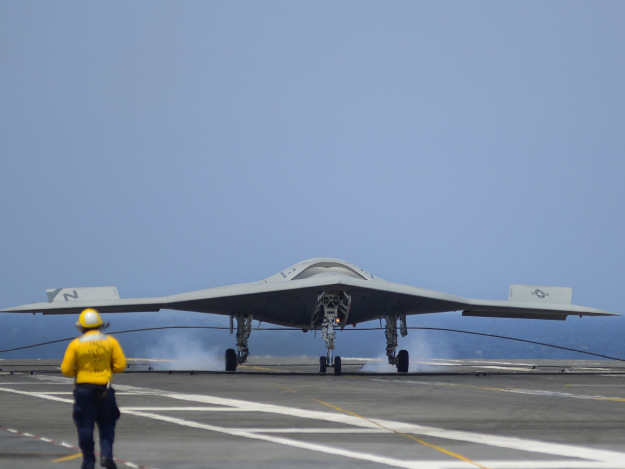
\includegraphics[height=5cm]{Figs/01_X47B_Landing.jpg}}\hspace{0.7em}%
	\subfloat[歼15着舰钩索的瞬间]{%
		\label{fig:22_J15Landing_Big}
		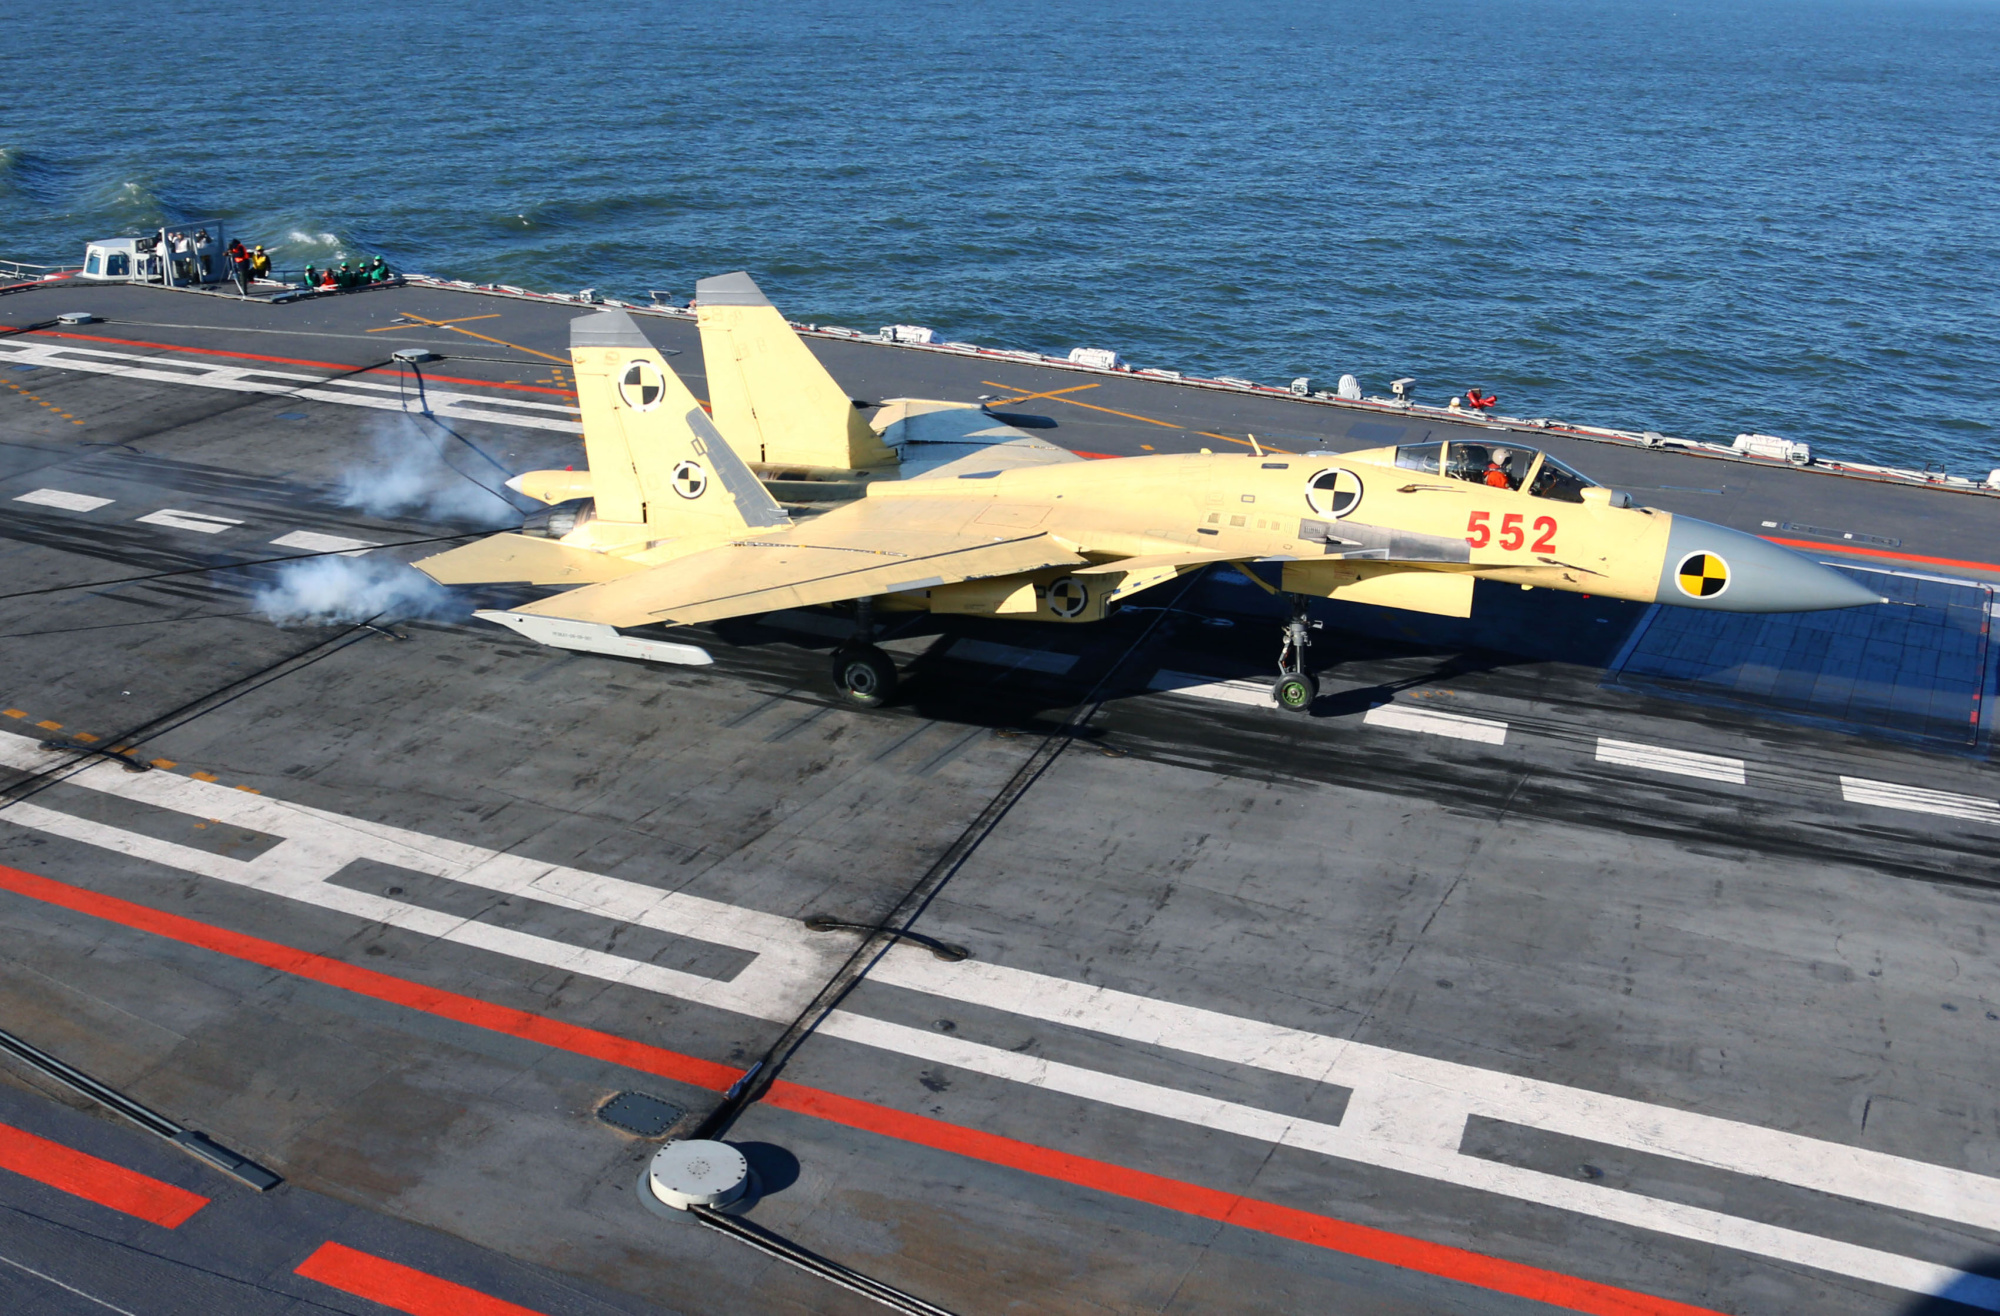
\includegraphics[height=5cm]{Figs/22_J15Landing_Big.jpg}}
	\caption{中美海军飞行器着舰瞬间}
	\label{fig:01_Landing}
\end{figure}

在舰载机降落过程中,飞行员除利用光学助降系统提供的信息进行修正外,航母舰舰载机着陆通常还依赖于人工辅助降落信息。在美航母上,通常由6人组成的着舰信号官(Landing Signal Officer,LSO)位于航母着舰区后部左舷,依靠视频监视系统所拍摄的实时图像及相应参数,通过无线电及灯光等多种手段对舰载机飞行员发出相应着舰指令(如图\ref{fig:20_LSO_USA}所示)。这6人分工和人员配置:(1)担当舰载机着舰引导操作的LSO;(2)利用飞行员助降视频(HUD)显控台引导飞机进场着舰顺序的助理LSO;(3)记录着舰成绩/等级的见习LSO;(4)担任舰内联络的下士联络员;(5)舰载机着舰前尾钩、起落架、襟翼状态的观察员;(6)负责监察着舰引导小组工作的负责人。而在公开的资料中,我国的有人机着舰也采用了类似LSO的人工辅助引导手段,其工作状态如图\ref{fig:21_LSO_China}所示。

\begin{figure}[htb]
	\centering%
	\subfloat[我国“辽宁号”航母上的LSO]{%
		\label{fig:21_LSO_China}
		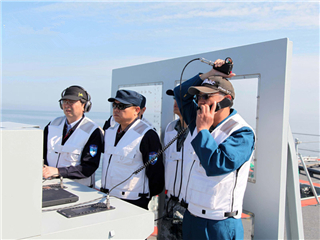
\includegraphics[height=4cm]{Figs/21_LSO_China.jpg}}\hspace{4em}%
	\subfloat[美军航母上的LSO]{%
		\label{fig:20_LSO_USA}
		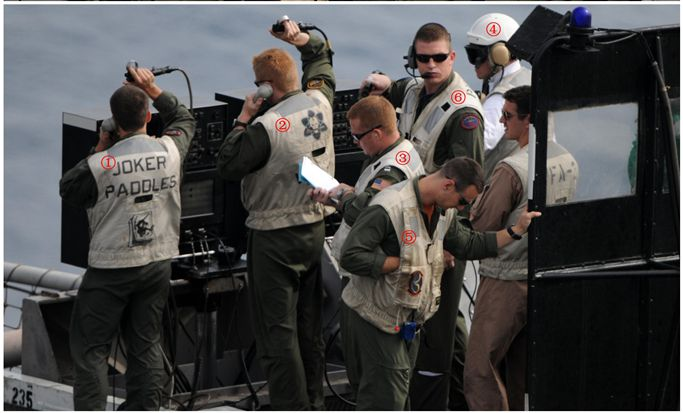
\includegraphics[height=4cm]{Figs/20_LSO_USA.jpg}}
	\caption{中美两国海军LSO工作图}
	\label{fig:21_LSO}
\end{figure}

无人机方面,在降落阶段无人机往往变成了“有人机”,一般会有多个人员进行操控和监视,以免出现差错。所以,本来希望减少人员工作负担的无人机,在降落阶段却往往成为让人担心的“微型炸弹”。为解决无人机的自主起降问题,早在2007年,美国诺斯鲁普·格鲁曼公司开始基于X-47B无人机和美国海军“无人作战航空系统-验证机”(UCAS-D)项目,开发和验证一种自主起飞/拦阻着舰型无人作战飞机。项目合同规定,诺格公司需要研制两架X-47B验证机,完成在航母上自主起降能力的验证,并在完成与航母一体化验证试验后,验证空中自主加油能力。如图\ref{fig:14_LandingAreaX47B2}所示,美国为开展相关研究,在Patuxent River试验基地展开岸基测试,并绘制了模拟甲板起降范围的模拟跑道(如图\ref{fig:10_LandingAreaX47B1}黄色箭头所示),这些细节体现了美国军方对这项技术的重视程度。
\begin{figure}[htb]
	\centering%
	\subfloat[位于海岸边的美军Patuxent River试验基地卫星图片]{%
		\label{fig:14_LandingAreaX47B2}
		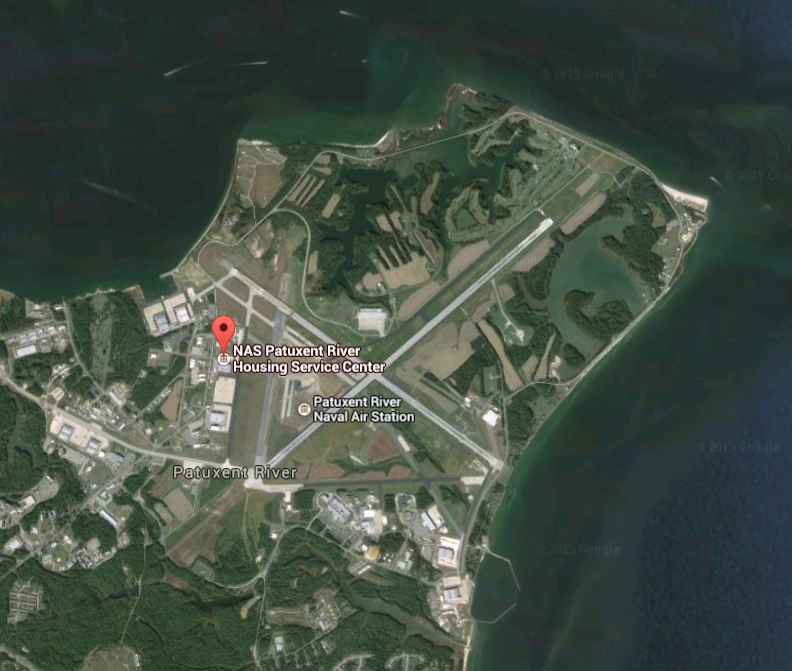
\includegraphics[height=6cm]{Figs/14_LandingAreaX47B2.jpg}}\hspace{0.7em}%
	\subfloat[黄色箭头所指为模拟航母甲板区域的专用跑道]{%
		\label{fig:10_LandingAreaX47B1}
		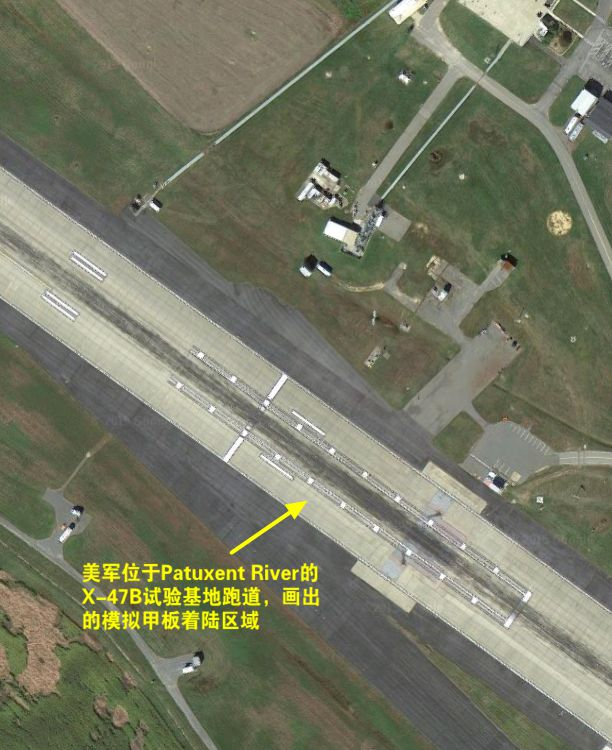
\includegraphics[height=6cm]{Figs/10_LandingAreaX47B1_1.jpg}}
	\caption{美军Patuxent River试验基地}
	\label{fig:14_LandingAreaX47B}
\end{figure}

在沉寂消息多年后,2013年7月,X-47B完成举世瞩目的首次航母自主降落,如图\ref{fig:01_X47B_Landing}所示)。根据公开资料显示\cite{X_47B},X-47B总共完成37次接触甲板测试(Deck Touchdown Test)和30次复飞(Touch-and-go)测试。在2014年3月,由于X-47B及其配套系统完成了人类历史上首次无人飞行器在航空母舰的全自主测试,“X-47B技术团队”获得美国航空协会最重要的“罗伯特·科利尔奖(Robert J. Collier Trophy)”\cite{X_47B_Award}。值得关注的是,该奖项曾经颁奖给诸多美国军用项目,如“全球鹰”无人机系统、“大黄蜂”战机系统、B2轰炸机系统等,由此可见X-47B及其配套系统在理论和工程上所具有的重要意义。此外,在各类报道中也特别提到:该系统精确的导航系统满足了飞行器降落在运动中的航母甲板上,具有里程碑意义\cite{X_47B_Report}。2014年8月,X47-B开展进一步测试,在完成与F/A-18F联合飞行验证后,在90秒内完成自主着舰、折叠机翼、撤出着舰区等一些列动作。其中,4次拦阻着陆,9次复飞再着陆。由于其优秀的控制性能,同月,美国海军计划利用X-47B开展空中自主加油的验证。根据公开资料判断,X-47B的降落除机载传感器外,舰载的JPALS或类似的雷达系统应当提供了辅助信息,如图\ref{fig:X47B_LandingOptical}所示。

\begin{figure}[htb]
	\centering%
	\subfloat[X-47B公布的视频中,跑道一侧的疑似毫米波雷达引导系统]{%
		\label{fig:09_X47BwithRadarGround}
		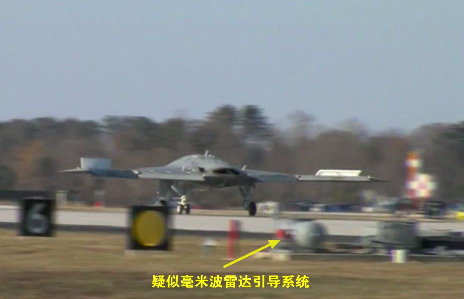
\includegraphics[height=5.2cm]{Figs/09_X47BwithRadarGround.pdf}}\hspace{1em}%
	\subfloat[X-47B公布的视频中,位于舰岛的疑似毫米波雷达引导系统]{%
		\label{fig:02_X47B_LanidngwithRadar1}
		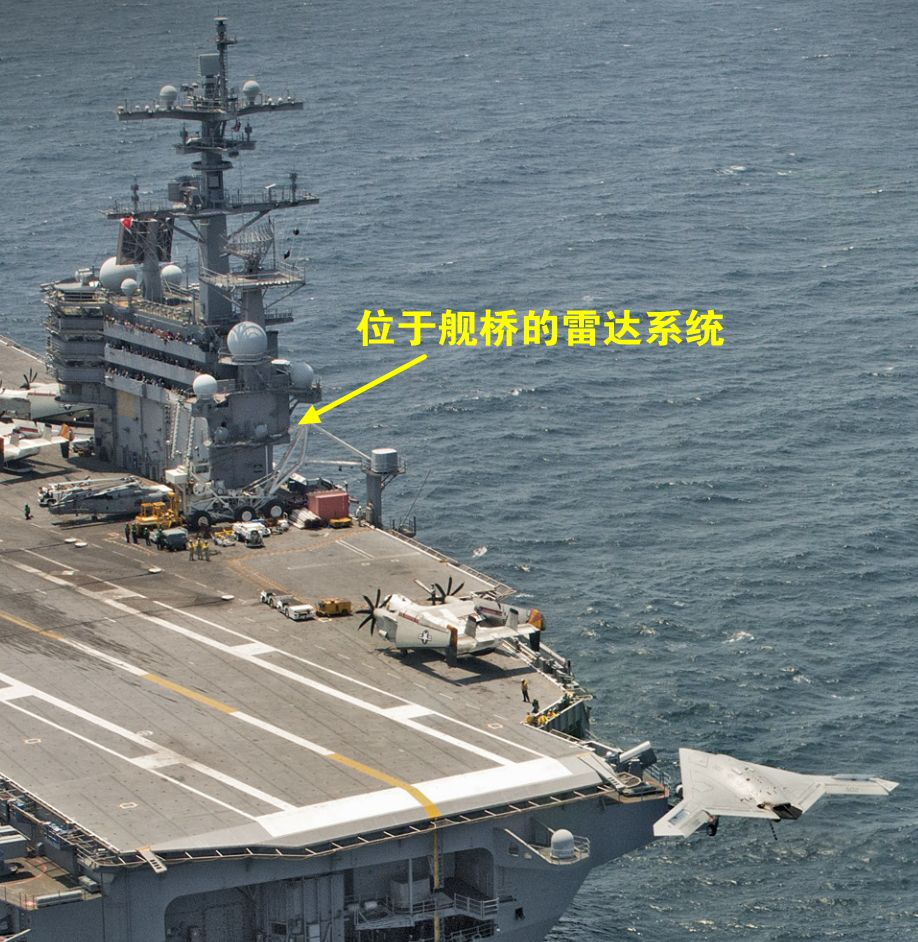
\includegraphics[height=5.2cm]{Figs/02_X47B_LanidngwithRadar1.jpg}}
	\caption{X-47B疑似使用的引导系统}
	\label{fig:X47B_LandingOptical}
\end{figure}



除X-47B这一机型之外,在2014年出版的《2030年的武器装备》\cite{2030equipment}一书中提到,作为美军太空机动飞行器的验证机型X-37B轨道飞行器(OTV, Orbital Test Vehicle),其在返回过程中,运用航空器的导航与指导技术,采用惯性导航和GPS的组合式导航方式,在接近跑道前,以20°的下滑角,350 km/h的速度进场,其降落过程和姿态与X-47B相似(如图\ref{fig:31_X37B_Landing}所示)。根据公开资料显示,X-37B的自主再入和着陆系统采用了惯性导航和GPS的组合式导航。截至到2014年10月17日,X-37B已经完成三次飞行试验,其再入与着陆技术得到波音公司和美国军方的认可。此外,根据2015年2月23日的公开报道,X-37B轨道测试飞行器团队(X-37B Orbital Test Vehicle Team)荣获2015年美国AIAA颁发的年度最高奖项——杰出贡献奖(Award for Excellent)\cite{X_37B}。在颁奖的公告中特别提到,自主降落技术是X-37B的关键技术之一。

\begin{figure}[htb]
	\centering%
	\subfloat[X-37B降落沿跑道方向正视图]{%
		\label{fig:31_X37B_Landing1}
		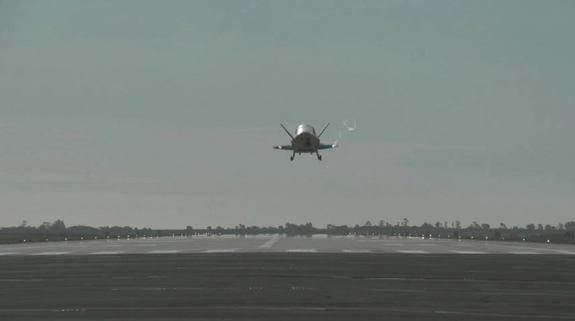
\includegraphics[height=4cm]{Figs/31_X37B_Landing1.jpg}}\hspace{0.7em}%
	\subfloat[X-37B降落侧视图]{%
		\label{fig:32_X37B_Landing2}
		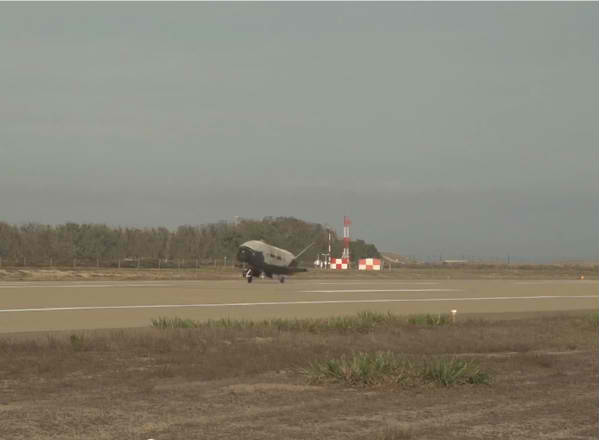
\includegraphics[height=4cm]{Figs/32_X37B_Landing2.jpg}}
	\caption{X-37B完成自主降落}
	\label{fig:31_X37B_Landing}
\end{figure}

综上所述,无人机自主起降技术,特别是舰载无人机自主起降技术是无人机广泛使用的基础和关键。能够在舰载环境,完成无人机的自主回收工作,具有很大的现实意义。


\section{军事和工业领域的引导降落系统}
\subsection{普通飞行器引导降落系统}
\subsubsection{仪表着陆系统}
在航空业发展初期,仪表着陆系统(ILS, Instrument Landing System)作为飞行器的主要着陆手段。该系统于1919年通过美国国家标准局的试验,并在二次大战期间得到广泛应用。1949年,国际民航组织规定仪表着陆系统作为着陆系统的国际标准。该系统主要由地面站和机载设备组成,主要通过机载接收机解算由地面航向信标和下滑信标独立产生的水平和交叉方向波束(波束频率不同),得到飞机的位置信息,即方位角、仰角和距离。该系统的示意图如图\ref{fig:07_ILS}所示。同时,民航组织根据需要,对不同气象条件下的进场标注进行了明确规定。其中,CAT I级别的高度主要通过气压计进行判读,CAT II和CAT III主要通过雷达高度计(Radio Altimeter)进行判读,不同级别的决断高度是飞行员做出是否复飞的基本准则。该系统的优点是具备较好的引导能力,可以为飞行员提供有效方位信息。但在当前电磁频谱环境复杂的机场附近,往往难以得到理想的引导控制精度,因此不能满足无人机系统的降落需求。该系统示意图如\ref{fig:07_ILS}所示。

\begin{figure}[htb]
	\centering%
	\subfloat[飞机在右偏,高度高于标准下滑曲线时的机载仪表显示]{%
		\label{fig:07_ILS1}
		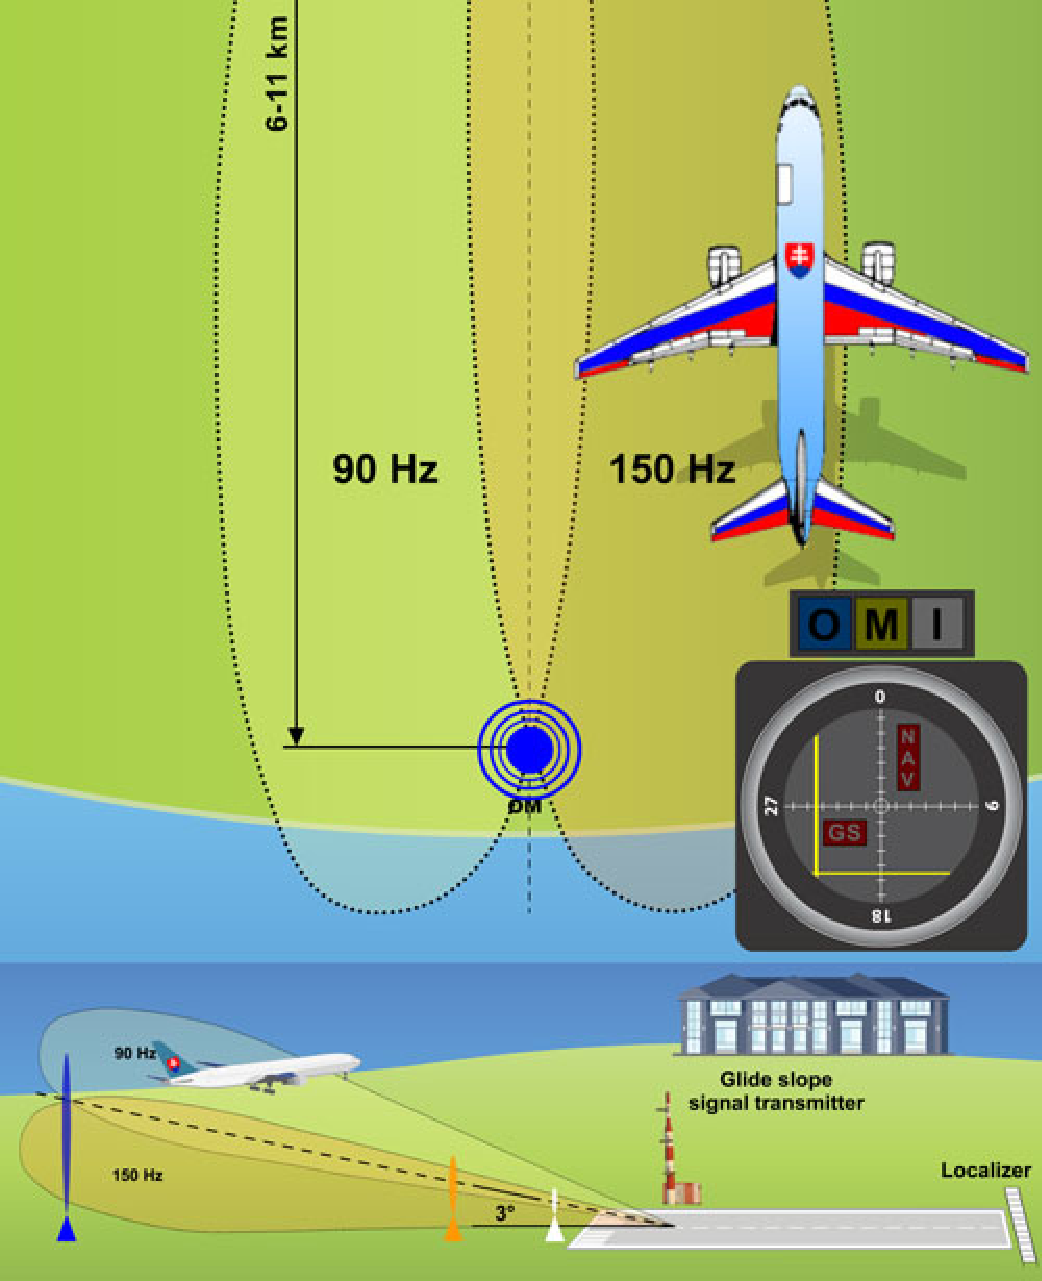
\includegraphics[height=7cm]{Figs/07_ILS1.pdf}}\hspace{4em}%
	\subfloat[飞机在左偏,高度低于标准下滑曲线时的机载仪表显示]{%
		\label{fig:08_ILS2}
		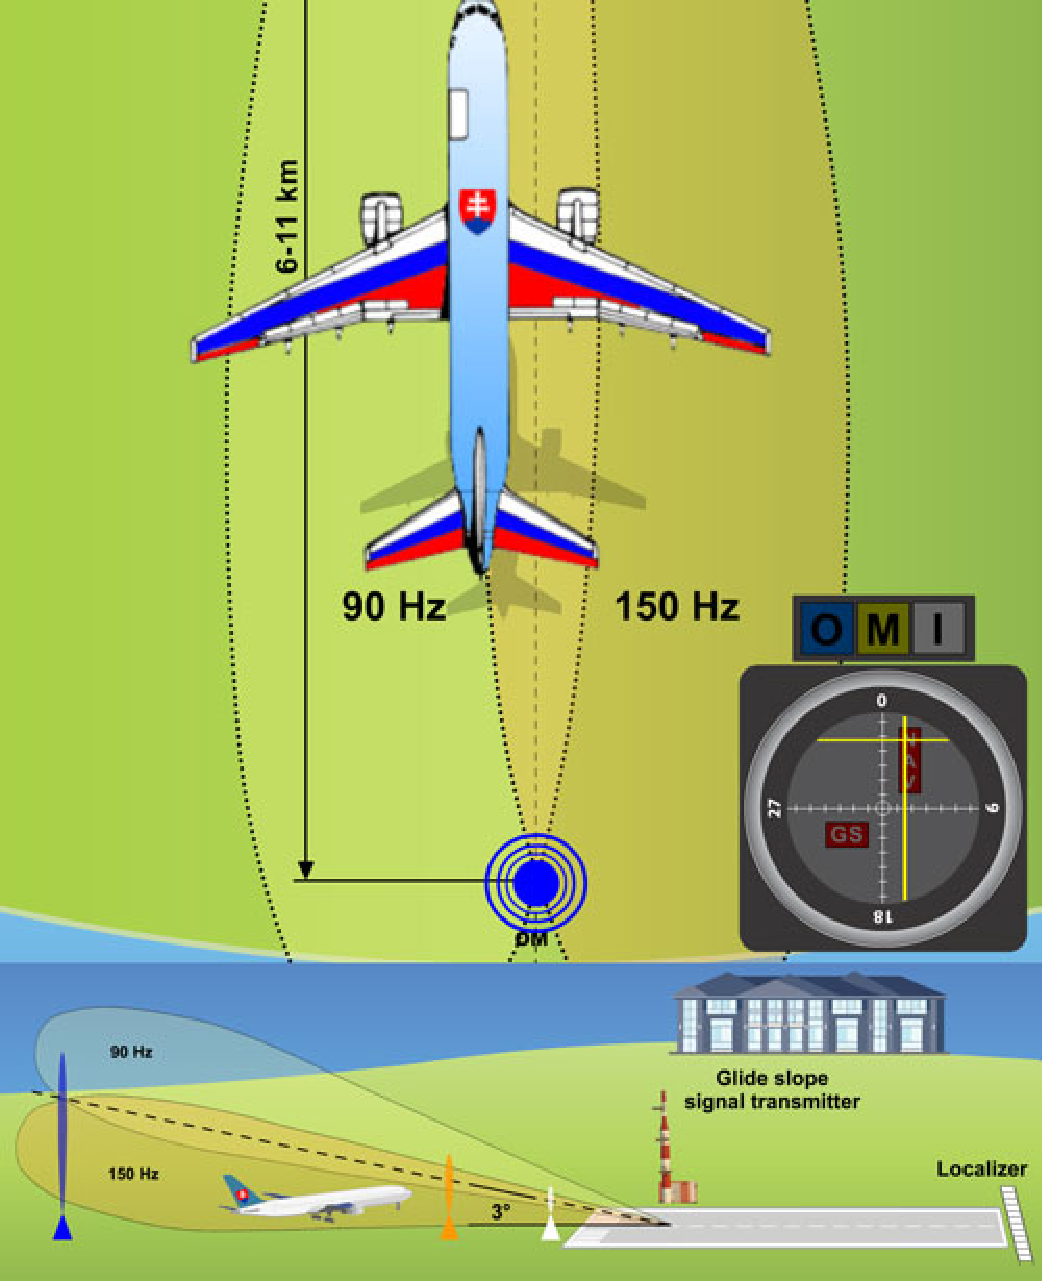
\includegraphics[height=7cm]{Figs/08_ILS2.pdf}}
	\caption{仪表着陆系统示意图}
	\label{fig:07_ILS}
\end{figure}

\subsubsection{雷达着陆系统}
随着二次大战对雷达在军事领域的广泛使用,美军在1943年研制了首套雷达着陆系统(GCA,Ground Control Approach),并于1946年拓展到民用领域。该系统通过地面引导雷达提供精确的位置信息,地面领航员根据雷达显示的下滑路径偏差与飞行员通话,进而操作飞机完成降落。随着技术发展,在雷达系统计算出下滑偏差后,可以根据飞机类型进行引导率计算,形成控制指令后反馈给飞机,协助飞行员或机载飞行系统完成下滑控制。这种方法也被称为“数据链+雷达”系统,至今仍然作为一种可靠的技术手段在航母和军用机场使用。

\subsubsection{微波着陆系统}
1978年,时间基准波束扫描技术(TRSB, Time Reference Scanning Beam)作为微波着陆技术的国际标准得到ICAO的认可。该系由地面方位台、仰角台、精密测距器和机载接收机组成。方位台和仰角台通过向空中发射扫描信号,机载接收机通过测量两次波束信号的时间间隔,得到飞机在空间的位置。但由于仪表着陆系统的广泛应用以及GNSS导航系统的迅猛发展,微波着陆技术的发展出现了一定的停滞。

\subsubsection{联合精密进近和着陆系统}
随着GPS和DGPS技术在美军的广泛应用,一套联合精密进近和着陆系统(JPALS)于2000年在地基完成测试实验。针对舰船本身和飞机都在运动,JPALS需采用双向的UHF数据链,将舰船测量到自身的GPS的位置,以及其摇摆、俯仰、偏航和向前运动的数据一并传给飞机,与此同时,飞机也将其GPS数据传回舰船。舰载的JPALS并不在意实际的位置误差,仅关注船和飞机偏离的量要相同,其着舰精度满足CAT III级别,纵向和横向精度控制在$1 \m$之内,能够完成航母着舰引导任务。在2005至2006年,JPALS开始替换现有的以雷达为基础的AN/SPN-46舰载精密进场着陆系统。这套系统还可用于舰上的空管,双向的数据链能使舰船以GPS跟踪、标注飞机方向。根据公布的合同要求,系统具备初始能力(IOC)时间为2019年,系统具备完全能力(FOC)时间为2030年。


\subsubsection{OPATS(Object Position and Tracking System)}
OPATS是瑞士RUAG宇航公司在1999年为瑞士空军开发研制的“目标定位跟踪系统”的简称,是一套基于激光技术的无人机自动着陆系统,用于瑞士空军的“巡逻兵”无人机。OPATS系统使用反射回来的激光信号对无人机进行跟踪,对目标无人机的动态位置进行连续测量跟踪,提供无人机在着陆阶段的可靠位置信息,并将高速更新的数据传输到地面站进行处,如图\ref{fig:15_OPTAS}所示。自1999年以来,RUAG已向全球范围内的众多用户交付了超过100套的OPATS系统。该系统的目标检测范围为35米至4000米,精度控制在1.5米。

\begin{figure}[htb]
	\centering%
	\subfloat[OPATS引导降落系统外场配置图]{%
		\label{fig:15_OPTAS1}
		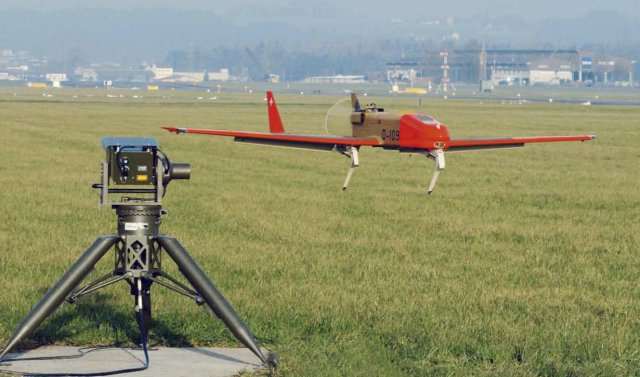
\includegraphics[height=4cm]{Figs/15_OPTAS1.jpg}}\hspace{4em}%
	\subfloat[OPATS引导降落系统框图]{%
		\label{fig:16_OPATS2}
		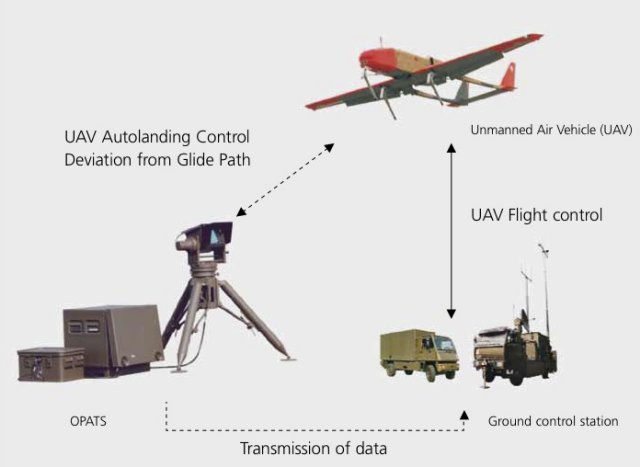
\includegraphics[height=4cm]{Figs/16_OPATS2.jpg}}
	\caption{OPTAS系统介绍}
	\label{fig:15_OPTAS}
\end{figure}


\subsubsection{光学引导系统}
光学助降系统主要依赖于“菲涅尔透镜”(Fresnel Lens)提供给飞行员相应的下滑曲线信息,以便飞行员操作飞机,即该引导系统是人在回路的引导方式。菲涅尔透镜有较好的聚焦性能,在同等焦距上由于传统球面透镜。由助降灯组和稳定平台组成,核心是位于中央的菲涅尔透镜和位于透镜两侧的水平基准灯。	舰载用的菲涅尔透镜系统(FLOLS, Fresenel Lens Optical Landing System)在传统的菲涅尔透镜基础上,将助降灯组与稳定平台结合。稳定平台的惯性系统可以检测舰船运动,使得射出的光束不受航母沉降摇摆的影响。在飞机进行着舰训练时,这套灯光组会释放出黄色、红色和橙色三种不同色彩光的下滑坡面,并以这三种光来界定高低位置。黄色光是高的下滑坡面,红色光是低的下滑坡面,橙色光是正确的下滑坡面。飞行员根据光所标定的位置在橙色光区域内下滑,就可以正确安全地着舰。


\subsubsection{基于UCARS的自主回收}
无人机通用自动回收系统(UAS Common Automatic Recovery System,UCARS)-V2系统(如图\ref{fig:29_UCARS})由内华达山脉公司(SNC)设计,为MQ-8B和MQ-8C火力侦察兵旋翼无人机的自主着陆提供引导控制。该系统是SNC的AN/UPN-51(V)无人机通用自动回收系统(UCARS)的改进型,并根据美军需求,拓展到其他型号的无人机引导降落,例如美国海军陆战队使用的先锋无人机。

该系统的主要传感器是毫米波雷达,该传感器也是军事和工业领域在引导无人机降落过程中使用最多的传感器质之一。毫米波雷达比普通的微波雷达体积更小,同时还具备波束窄和抗干扰能力强的特性;相比于红外传感器,毫米波雷达对于雨雾天气和灰尘的穿透性更强。UCARS系统主要由机载应答系统和舰载跟踪系统组成。跟踪传感器可以检测并计算无人机相对于期望降落点的位置信息,并向无人机提供降落平台的位置和运动状态数据,便于机载系统的导航和控制。目前UVARS系统有V2改进版,该版本使得无人机具备自主降落能力,减少了无人机飞行员的干预。此外,它还具备船舶运动稳定设备,以满足不同海况下的运行需求,该系统的引导控制精度在2.5厘米左右。系统的地基和舰载配置情况如图\ref{fig:29_UCARS}所示。 

\begin{figure}[htb]
	\centering%
	\subfloat[UCARS引导庞巴迪CL-227降落]{%
		\label{fig:29_UCARS1}
		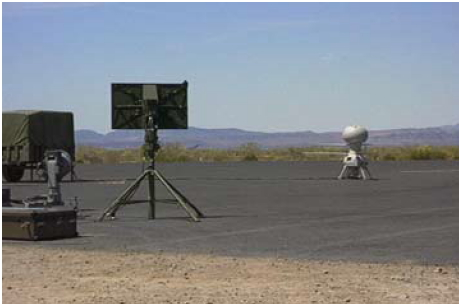
\includegraphics[height=4cm]{Figs/29_UCARS1.jpg}}\hspace{1em}%
	\subfloat[UCARS引导MQ-8B降落]{%
		\label{fig:30_UCARS2}
		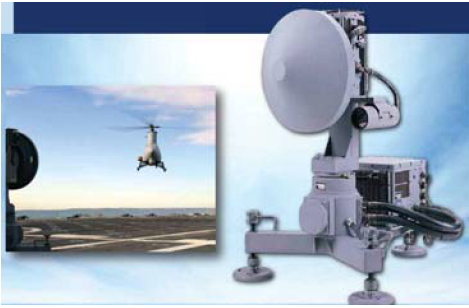
\includegraphics[height=4cm]{Figs/30_UCARS2.jpg}}
	\caption{无人机通用自动回收系统(UCARS)}
	\label{fig:29_UCARS}
\end{figure}

\subsubsection{无人机甲板起降引导系统}
法国DCNS公司开发的无人机直升机甲板起降引导系统(SADA\footnote{此处为法语缩写,Systèmed’Appontage et de Décollage Automatique})\cite{DCNS}使用红外传感器精确跟踪无人机,同时发出飞行指令调整航线直到确保无人机的“鱼叉”式着陆装置对准降落格栅的中心。2008年10,SADA成功将一架奥地利西贝尔公司研制的“坎姆考普特”(Camcopter)S-100无人直升机以自主模式降落在一艘正在地中海航行的法国海军驱逐舰“蒙特卡姆”号(Montcalm)上。该系统的引导控制精度约$30\ cm$。

\begin{figure}[!tb]   
	\centering	
	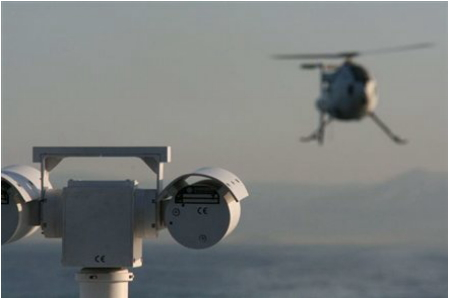
\includegraphics[width=0.5\textwidth]{Figs/24_SADA_Landing.jpg}
	\caption{SADA系统引导无人直升机着舰 }
	\label{fig:24_SADA_Landing}
\end{figure}


\subsubsection{基于D2AD自动甲板起降系统}
2011年,法国DCNS公司和Thales 公司完成无人机直升机在甲板自主降落(D2AD\footnote{此处为法语缩写,Démonstration d'un système d'appontage et d'atterrissage pour drones})的测试。此次海试使用法国海军“拉斐尔”级护卫舰和一架波音H-6U“小鸟”旋翼无人机,实验标志着 D2AD项目为期 4 年的技术验证成果。D2AD系统包括“飞行”部分和“地面”部分,“飞行”部分是无人机的指引标,“地面”部分在飞行甲板使用传感器进行船体运动预报,是无人机的引导站(如图\ref{fig:25_D2AD})。D2AD不依赖于任何卫星定位系统,能够保证垂直起降无人机在舰船上的安全使用。

\begin{figure}[htb]
	\centering%
	\subfloat[D2AD自主甲板降落系统]{%
		\label{fig:25_D2AD_1}
		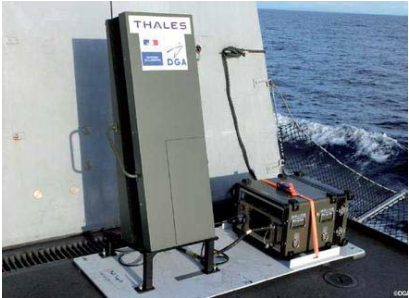
\includegraphics[height=4cm]{Figs/25_D2AD_1.jpg}}\hspace{0.1em}%
	\subfloat[H-6U“小鸟”旋翼无人机]{%
		\label{fig:26_D2AD_2}
		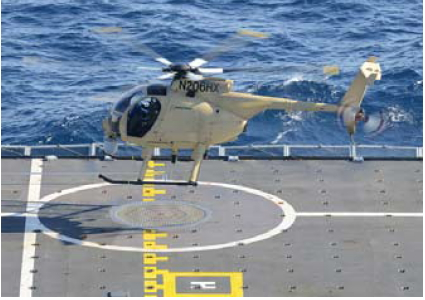
\includegraphics[height=4cm]{Figs/26_D2AD_2.jpg}}\hspace{0.1em}
	\subfloat[机载指引标]{%
		\label{fig:27_D2AD_3}
		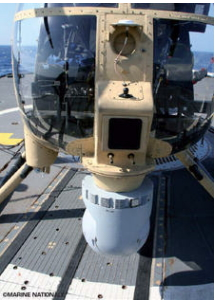
\includegraphics[height=4cm]{Figs/27_D2AD_3.jpg}}
	\caption{D2AD机载引导系统基本构成}
	\label{fig:25_D2AD}
\end{figure}

\subsubsection{基于DeckFinder的降落系统}
2013年6月,奥地利西贝尔电子设备公司的“坎姆考普特”S-100 无人直升机配装欧洲航宇防务集团(EADS)阿斯特里姆公司的“甲板发现者”(DeckFinder)区域定位系统,在一周的时间内完成了一系列旨在演示验证GPS干扰环境中无人机自动起飞与回收能力的飞行试验。“甲板发现者”系统\cite{Deckfinder}包括地面部分和机载部分,其中地面部分包括6台射频发射机,机载部分包括1台接收机。该系统的测距不依赖于GPS,可为航空器提供高精度的三维相对位置信息。根据公布的技术细节,该系统的工作范围约为$1.1\ km$,降落阶段精度优于$20\ cm$,工作频率不低于$15\ Hz$。
\begin{figure}[!tb]   
	\centering	
	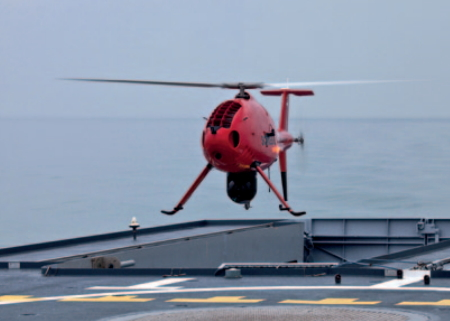
\includegraphics[width=0.5\textwidth]{Figs/28_Deckfinder.jpg}
	\caption{DeckFinder在GPS干扰环境下引导S-100无人机降落}
	\label{fig:28_Deckfinder}
\end{figure}

\subsubsection{基于JPALS的引导降落}
% X-47B
作为固定翼无人作战飞机,X-47B无人机面临着与其他无人机同样的难题:回收过程复杂。根据海军科技网站(Naval Technology)公布的消息\cite{X_47B_UCAS},X47-B的引导控制系统有较强的自主性,其导航系统主要由GPS和视觉系统组成。为提高智能化程度,X47-B还配备了光学系统、红外系统、SAR雷达(SAR, Synthetic Aperture Radar)、地面目标指示器(Ground mMving Tagret Indicator)和海面目标指示器(Maritime Moving Target Indicator)等设备。此外,在自主降落过程中,系统遵循预设的下降曲线对飞机进行引导和控制,操作员只是监视整个下降过程。虽然X-47B使用的具体引导降落方式没有公开,但通过公开视频和图像分析(如图\ref{fig:X47B_LandingOptical}所示),X-47B的自主着舰也应用了类似引导系统。

通过阅读相关资料并分析,该联合精确进场与着舰系统(JPALS)由处理、维修和监测系统,UHF数据链,惯性传感器和GPS传感器等组成,可以实现高可靠性和可用性。JPALS将与AN/TPX-42空中交通管制雷达、AN/SPN-46自动着舰系统、AN/SPN-41着舰辅助雷达、着舰信号官显示系统、改进型菲涅耳透镜光学着舰系统、航空数据管理和控制系统集成。2011年7月,F/A-18D“大黄蜂”战机在“艾森豪威尔”航空母舰上实现无人控制自主降落。

% ----- MQ-8B/C
2006年1月,MQ-8B完成了第一次在两栖登陆舰USS Nashville的舰载着陆,实验海域为Chesapeake Bay。2014年8月27日,MQ-8C“火力侦察兵”无人直升机在文图拉县海军基地完成着舰试验。

\subsection{无人机回收方式概述}
在X-47B无人机成功阻拦降落之前,世界各国在舰载无人机回收方面普遍采用的方法是:伞降回收、撞网回收、打捞回收和钩绳回收等。其中,撞网回收和钩绳回收对无人机回收控制精度提出更高要求,需要无人机自身或舰基系统具有较好的引导和控制能力。

\subsubsection{伞降回收}
伞降回收就是利用降落伞回收无人机。无人机从飞行状态到安全回收,整个过程自动完成,对操作人员要求较低。这种回收方式操作简单,是小型无人机回收的一种重要方式,适合对落点没有特殊要求的回收。采用轮式着陆的无人机也可使用伞降回收作为应急回收方案。采用水上伞降回收时,要考虑到无人机落入水中后对机身和内部设备的影响。

\subsubsection{撞网回收}
使用拦截网系统回收无人机是目前小型无人机较普遍采用的回收方式之一。无人机在降落阶段,通过降低高度和减小速度,撞向由弹性材料编制成的阻拦网。美国RQ-2“先锋”无人机和“银狐”无人机均采用
这类回收方式,如图\ref{fig:34_RQ2_Pioneer_Landing}所示。
\begin{figure}[!tb]   
	\centering	
	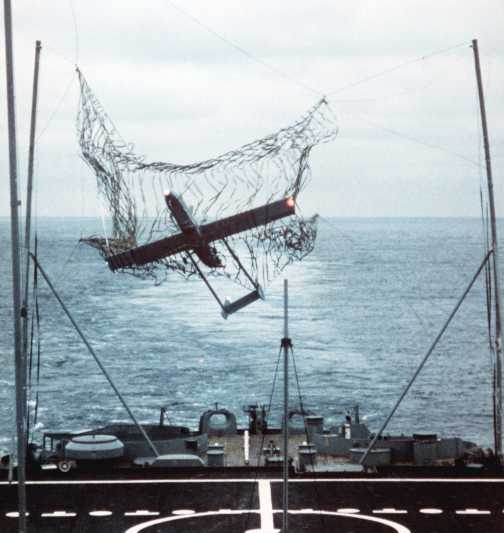
\includegraphics[width=0.4\textwidth]{Figs/34_RQ2_Pioneer_Landing.jpg}
	\caption{RQ-2在舰船完成撞网回收}
	\label{fig:34_RQ2_Pioneer_Landing}
\end{figure}

% Bat UAS
%翼展4.26 m、极长2.0 m、最大起飞重量159 kg、有效载荷34 kg。
%Shadow
%Poineer

\subsubsection{钩绳回收}
该回收方法使用垂直悬浮钢丝的天钩技术。钢丝可以自由的悬浮在吊杆上或者通过风筝把它升起,同时在无人机的翼尖上固定一个自锁的钩子。无人机进场时,径直地飞向钢丝,以便钢丝碰到其中一个机翼的前缘,然后滑向翼尖,通过钩子便可以把无人机锁住。由于航母的摆动幅度通常会限制为横摇2-3度,纵摇1-1.5度,而中小型船只稳定性要差得多,因此必须在横摇13度,纵摇5-6度的恶劣环境下,相比撞网回收,钩绳回收的引导控制需求更高,需要确保无人机在一米大小的回收窗口准确降落。

RQ-21A在2010年称为美国小型战术系统(Small Tactical Unmanned Aircraft System)项目的主力机型,该飞机具备陆基和海基起降能力,能够完成战术侦察、监视、目标指示(Reconnaissance, Surveillance and Target Acquisition,RSTA)功能,其模块化设计可快速替换不同传感器并完成部署。2014年7月,美国海军开始使用RQ-21A系统进行海上综合测试。该型无人机采用钩绳回收方式,如图\ref{fig:33_RQ21_Landing}所示。此外,“扫描鹰”无人机也采用此类方式回收,如图\ref{fig:35_Eagle_Scanner_Landing}所示。

\begin{figure}[htb]
	\centering%
	\subfloat[RQ-21在舰船回收]{%
		\label{fig:33_RQ21_Landing}
		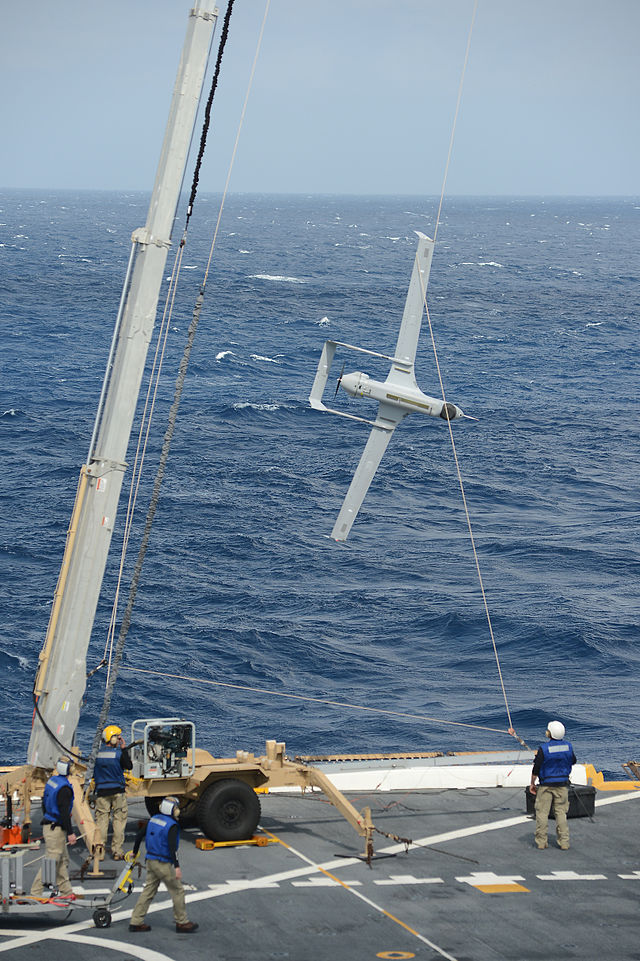
\includegraphics[height=6cm]{Figs/33_RQ21_Landing.jpg}}\hspace{0.1em}%
	\subfloat[“扫描鹰”无人机在舰船回收]{%
		\label{fig:35_Eagle_Scanner_Landing}
		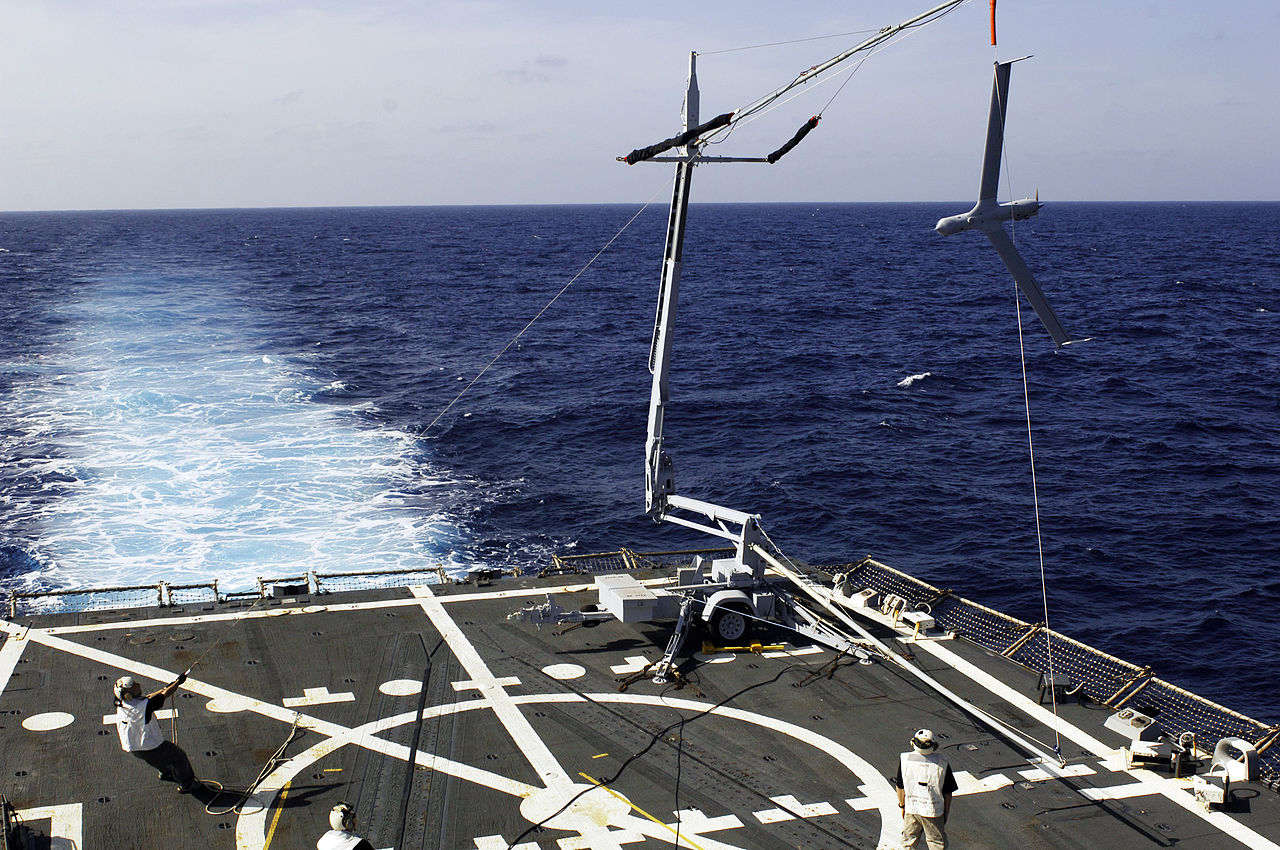
\includegraphics[height=6cm]{Figs/35_Eagle_Scanner_Landing.jpg}}\hspace{0.1em}
	\caption{采用钩绳回收方式的无人机}
	\label{fig:33_RQ21withScanner_Landing}
\end{figure}


\section{学术研究领域的无人机引导降落系统}
由于可见光摄像机成本低廉的特点,基于图像信息的无人机引导和控制在无人机实际应用中扮演十分重要的角色。例如,利用机载摄像机来完成感知规避任务\cite{mejias2010vision}、监视和跟踪任务\cite{campoy2009computer}\cite{mejias2006visual}、自主起飞和降落任务\cite{saripalli2002vision}、实时建图与定位任务(SLAM)\cite{weiss2011monocular}等。此外,通过图像信息对无人机自身位置和姿态进行估计也是今年来的研究重点和热点。比如在空中加油领域、无人机定点区域着陆等。2014年,针对视觉在无人机自主降落领域的研究现状,文章\cite{kong2014vision}系统总结了当前37个世界各地研究单位的工作,总结表格详见附录。本节只针部分内容进行概述。

\subsection{机载传感器引导降落系统} 

早在2003年,Shakernia\cite{shakernia2003vision}的博士论文中提出一种基于视觉的旋翼无人机(Yamaha R-50)的自主降落方案,该方案通过识别放置于六自由度运动平台上的合作标志完成自主降落(如图\ref{fig:chp01_06_shakernia_landing}所示)。其中,通过识别合作标志中的焦点,并使用Linear Two-view Motion Estimation, Non-linear Two-view Motion Estimation和Multi-view Planar Algorithm方法对飞机的位置和姿态进行估计。上述三种方法可以较好的解决特征点共面的飞机和位置姿态估计问题,通过仿真和户外试验,验证了系统的有效性和鲁棒性(位置偏差小于0.05米,角度偏差小于0.5°),但对于非合作目标的识别,不具备求解的通用性。

\begin{figure}[!tb]   
	\centering	
	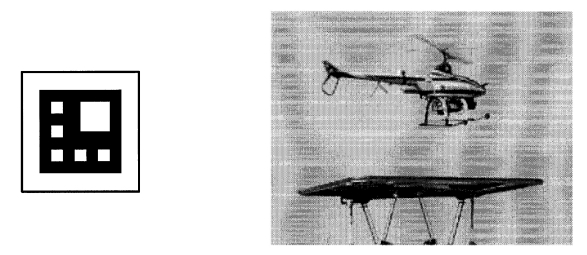
\includegraphics[width=\textwidth]{figs/chp01/chp01_06_shakernia_landing.pdf}
	\caption{基于合作标识的无人直升机自主降落系统}
	\label{fig:chp01_06_shakernia_landing}
\end{figure}


2009年,朱建明\cite{Zhu_Master_2009}对传统“H”形合作目标进行改进将“H”形图标的上端开口封住,改进后的图标能够克服“H”形图标缺乏有方向性的缺点,在地标图案分割的基础上,采用基于灰度变化的角点检测方法,提取合作标志的特征点。

2010年之后,该领域的研究逐渐增多。韩国科学技术院(Korea Advanced Institute of Science and Technology,KAIST)提出一种应用于小型无人机上的视觉引导着陆系统通过视觉引导无人机飞行至安装在地面上的红色圆拱形安全气袋中\cite{huh2010vision},原理如图\ref{fig:chp01_05_korea_landing}所示。
\begin{figure}[!tb]   
	\centering	
	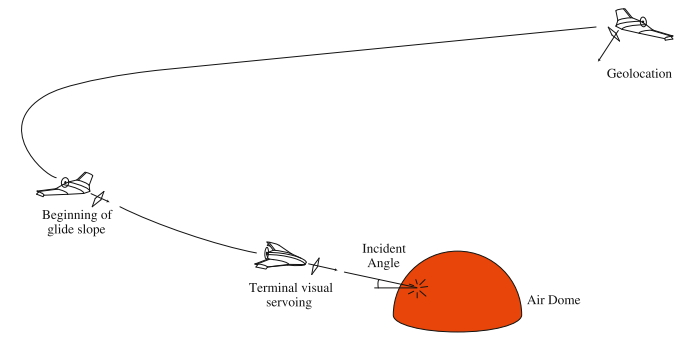
\includegraphics[width=\textwidth]{figs/chp01/chp01_05_korea_landing.pdf}
	\caption{基于红色标志物的无人机回收系统示意图}
	\label{fig:chp01_05_korea_landing}
\end{figure}

李宇\cite{Li_Master_2012}设计了一种由6个圆心已标识出来的红色圆圈组成的合作标志,通过基于仿射不变矩和SVM分类器实现着陆地标的识别,如图\ref{fig:chp01_04_six_circle_landing_pattern}所示。
\begin{figure}[!tb]   
	\centering	
	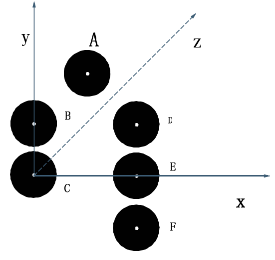
\includegraphics[width=0.4\textwidth]{figs/chp01/chp01_04_six_circle_landing_pattern.pdf}
	\caption{六个圆形合作标识}
	\label{fig:chp01_04_six_circle_landing_pattern}
\end{figure}

H. Jin Kim等人\cite{kim2013fully},针对小型固定翼无人机提出了一种基于机载视觉的撞网回收系统。该系统采用颜色分割和形态学等图像处理算法,通过机载摄像头对无人机回收网进行检测和识别;通过几何位置分析,判断无人机当前的方位信息,设计无人机引导率和控制率;地面控制系统可以向无人机发送控制命令并监测无人机的飞行状态。

德国宇航局在2015至2016年进行了HALE(High Altitude Long Endurance) UAV在运动汽车顶部回收的实验测试,该型号无人机的翼展为$3.3\ m$,最大起飞重量为$21.5\ kg$。该无人机在距离地面车辆$300\ m$左右的距离捕获地面移动车辆,随后地面移动车辆加速至合适的速度,满足无人机的回收需要。在回收过程中,无人机的引导方式主要通过机载摄像机对汽车顶部的合作标识(二维码)进行识别,进而实现相对位置的解算,完成自主降落\cite{Muskardin2016}。由于合作标识的尺寸和机载相机视场角的约束,无人机检测到地面目标点的距离较短,系统有效工作范围较小。
\begin{figure}[htb]
	\centering%
	\subfloat[无人机在回收末状态时,与汽车的速度保持相同]{%
		\label{fig:07_ILS1}
		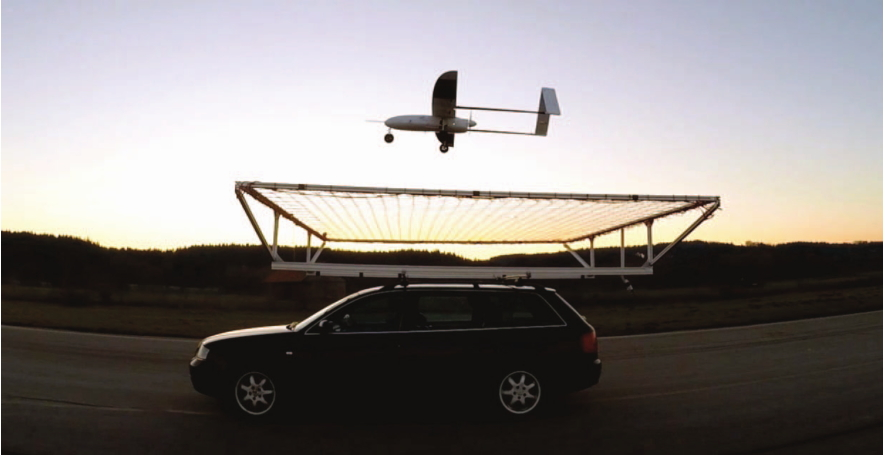
\includegraphics[height=3.5cm]{figs/chp01/chp01_01_DLR_Landing.pdf}}\hspace{0em}%
	\subfloat[机载传感器通过识别车顶的合作标识,实现相对位置的解算]{%
		\label{fig:08_ILS2}
		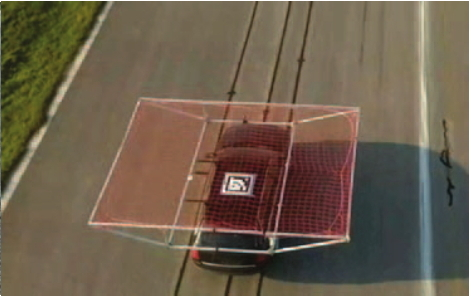
\includegraphics[height=3.5cm]{figs/chp01/chp01_02_DLR_Landing_with_tag.pdf}}
	\caption{德国宇航局车载无人机回收试验图}
	\label{fig:07_ILS}
\end{figure}

2016年5月,卡内基梅隆大学的研究者发布了最新无人直升机降落在海面移动平台\cite{Grocholsky2016}的工作。无人机上装载了长波红外传感器,该传感器适应雨雾天气,最远探测海面移动平台的距离为1.2海里(约2.22公里)。无人机从500米开始,对海面移动平台进行位置估计,并逐渐靠近该平台。在距离195米左右时,机载可见光传感器可以识别位于降落平台的合作标识,并具备对该平台姿态进一步估计的能力,其识别效果如图\ref{fig:chp01_03_CMU_Sea_Landing}所示。在最后50米的距离,激光传感器通过对甲板的三维空间扫描,实现厘米级的位置解算精度。

\begin{figure}[htb]   
	\centering
	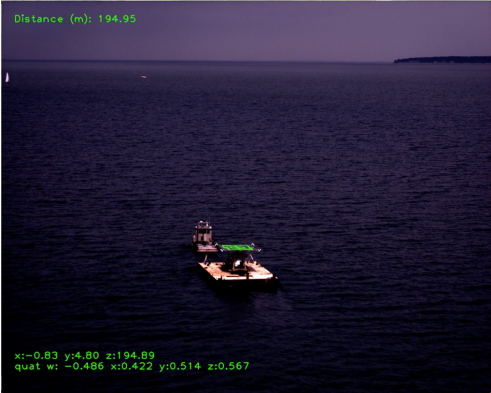
\includegraphics[width=0.6\textwidth]{figs/chp01/chp01_03_CMU_Sea_Landing.pdf}
	\caption{卡内基梅陇大学直升机机载视觉传感器在降落过程中的对降落目标位置和姿态的解算}
	\label{fig:chp01_03_CMU_Sea_Landing}
\end{figure}

此外,通过机载传感器直接识别机场跑道,也可以视为一种基于合作标识的降落方法。德国宇航中心DLR飞行控制研究所提出了一种利用可见光、红外或雷达图像中的跑道信息估计固定翼飞机的相对位置的方法,并在其研制的ESVS(Enhanced and Synthetic Vision)平台上得到验证\cite{doehler2003robust}。

\subsection{地基传感器引导降落系统} 

用于户外的地基引导系统并不常见,国防科技大学在2011年,提出一种地基引导系统\cite{Ding_master_2011},该系统通过地面摄像机识别无人机上悬挂的红外标记,完成对无人机的引导降落。在目标无人机沿下滑曲线下降至$400\ m$左右的距离时,引导系统开始工作,此时的无人机高度约为$50\ m$;在距离相机$50\ m$距离时,系统的高度分辨率为$0.032\ m$,水平分辨率为$0.26\ m$。该系统的排布如图\ref{fig:chp01_07_ding_master}所示。

\begin{figure}[htb]   
	\centering
	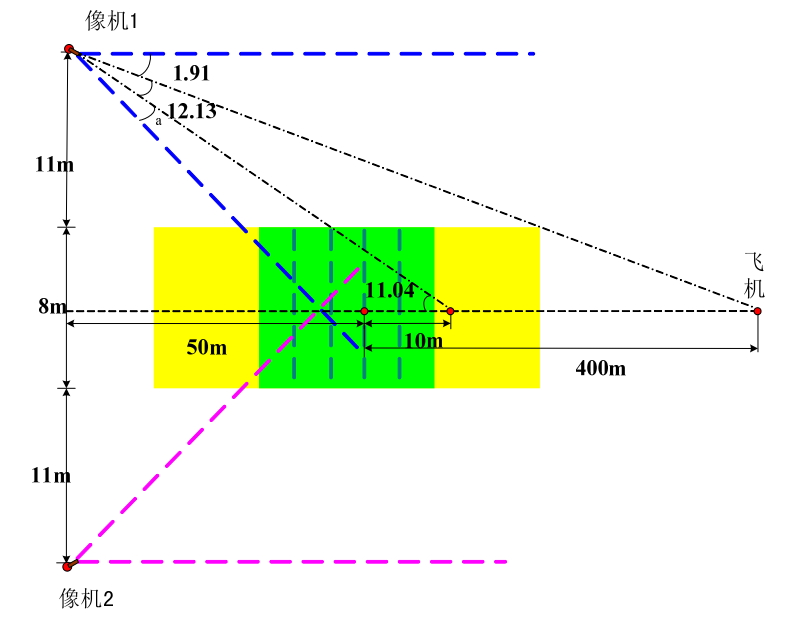
\includegraphics[width=0.6\textwidth]{figs/chp01/chp01_07_ding_master.pdf}
	\caption{地面引导系统排布示意图}
	\label{fig:chp01_07_ding_master}
\end{figure}

此外,该研究组还提出了采用多台固定焦距摄像机分区域接力测量的方案如图\ref{fig:chp01_08_gui_doctor}所示\cite{gui_doctor_2013}。视觉引导系统由三组摄像机选取不同的焦距,分别观测远场、中场和近场区域,保证相邻两组摄像机视场有一定的重叠区域,并覆盖无人机的下降区域。

\begin{figure}[htb]   
	\centering
	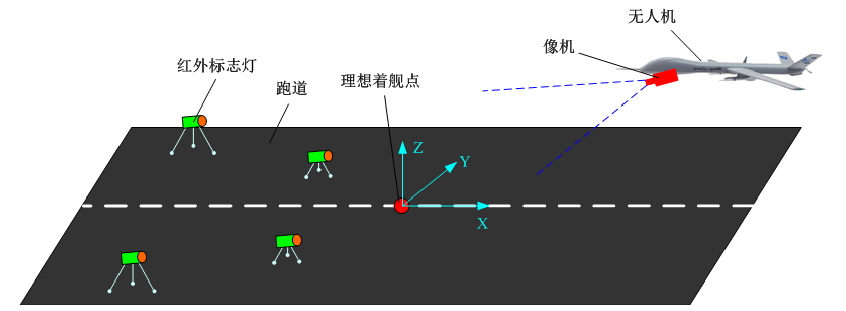
\includegraphics[width=0.6\textwidth]{figs/chp01/chp01_08_gui_doctor.pdf}
	\caption{地基多相机引导系统示意图}
	\label{fig:chp01_08_gui_doctor}
\end{figure}

文献\cite{Garcia-Pardo2002}给出了一种基于步进电机和网络摄像头结合的引导设备,可以对微小型无人机进行跟踪,但其视场角受到步进电机的约束。Martinez\cite{Martinez2010}提出了一种三目摄像机系统,如图\ref{fig:chp01_09_three_ground_landing}所示,该系统可以检测无人机的特征点,得到位置信息,但由于构型限制,该系统只适用于旋翼直升机的降落。美国斯坦福大学(Stanford University)\cite{Saripalli2003}使用两个或以上的相机得到了距离$40\ m$外,位置误差约$25\ cm$的视觉系统,但文献中没有具体描述系统的具体结构。日本千叶大学(Chiba University)的研究者\cite{PEBRIANTI2010}使用利用Bumblebee立体视觉传感器,成功将一架四悬翼从$6\ m$的高度引导降落。

\begin{figure}[htb]   
	\centering
	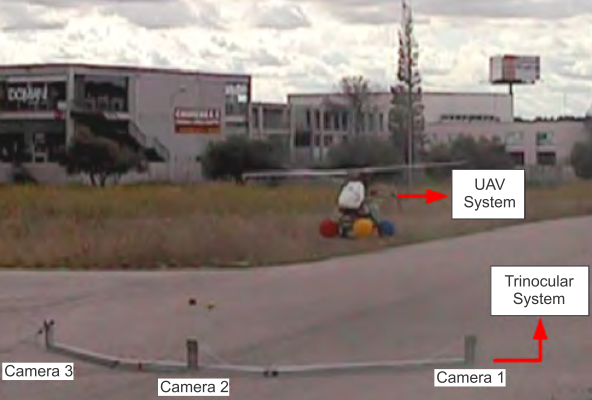
\includegraphics[width=0.7\textwidth]{figs/chp01/chp01_09_three_ground_landing.pdf}
	\caption{地面引导系统排布示意图}
	\label{fig:chp01_09_three_ground_landing}
\end{figure}

\section{本文的主要工作、贡献和结构}
本文瞄准固定翼无人机着舰回收的实际需求,重点研究着舰引导控制的系统架构、机理建模、关键算法与综合验证,主要工作和贡献如下:

(1)提出一种舰基通用的多传感器无人机回收引导系统。该系统主要有两个独立引导单元组成,每个引导单元配备一个二自由度转台和可见光相机、红外相机等多个传感器。两个独立引导单元的排布可以根据目标无人机的大小和检测距离进行优化配置。本文针对该系统独立分布在跑道两侧的特点,通过对目标位置解算理论推导、误差分析和实验验证,证明了在无人机降落过程中,使用上述引导系统的可行性。

(2)提出检测-跟踪-学习相融合的无人机降落过程中实时目标跟踪和位置解算框架。针对引导无人机降落过程中,无人机目标尺度快速变化问题,通过改进基于形态学滤波的图像预处理方法,TLD目标跟踪框架和基于主动轮廓的目标位置修正方法,结合转台运动位置和无人机运动的估计,能够准确解算出无人机在降落过程中相对于舰船的位置信息,满足无人机引导和控制系统的需要。

(3)设计基于非线性模型预测控制(NMPC)和总能量控制(TESC)的无人机着舰控制系统。由于无人机机载设备运算能力的约束,本文设计了内环控制器和外环控制器来实现无人机的自主降落。其中内环控制器由PI和PD控制器组成,完成对无人机姿态的控制;外环控制器由非线性模型预测控制器(NMPC)和总能量控制器(TESC)组成,针对基于Dubins Path生成的降落曲线进行跟踪。

(4)设计并实现无人机舰载着舰系统仿真环境并进行户外实验验证。本文基于机器人操作系统(Robot Operating System,ROS)和Gazebo仿真环境构建了无人机舰载着陆软件在回路仿真系统(SITL)和硬件在回路仿真系统(HIL)。该仿真环境能够满足上述算法的验证需求。通过二自由度转台与多传感器的组合配置,实现在地面机场和水面环境对小型和中型固定翼无人机的引导和自主降落。

本文各个章节的结构图如图\ref{fig:chp01_10_thesis_structure}所示。
\begin{figure}[!h]   
	\centering	
	\includegraphics[width=\textwidth]{figs/chp01/chp01_10_thesis_structure.pdf}
	\caption{本文的组织结构图}
	\label{fig:chp01_10_thesis_structure}
\end{figure}

\chapter{无人机着舰环境数学建模}
\label{chap:main}
无人机着舰的过程设计到无人机系统和舰船系统两大部分,因此为了研究这两部分直接的关系,必须对降落过程进行适当的数学模型\cite{beardsmall},以利于对无人机控制和引导系统进行数学仿真和物理实验。

\section{无人机系统坐标系定义}


\subsection{系统惯性坐标系}
系统惯性坐标系(Inertial Frame,$\mathcal{F}^i$),该坐标系一般定义位于地球表面的一点,三个轴的方向$(\mathbf{i}^i, \mathbf{j}^i,\mathbf{k}^i)$与地球的北向、动向和指向地心方向相同,即NED坐标系。通常该坐标系定义为飞机的起飞点或降落点,本文中我们选用无人机被舰船引导系统捕获时,舰船的此刻所在的点为原点,如图\ref{fig:chp02_01_sys_interial_frame}所示。
\begin{figure}[htb]   
	\centering
	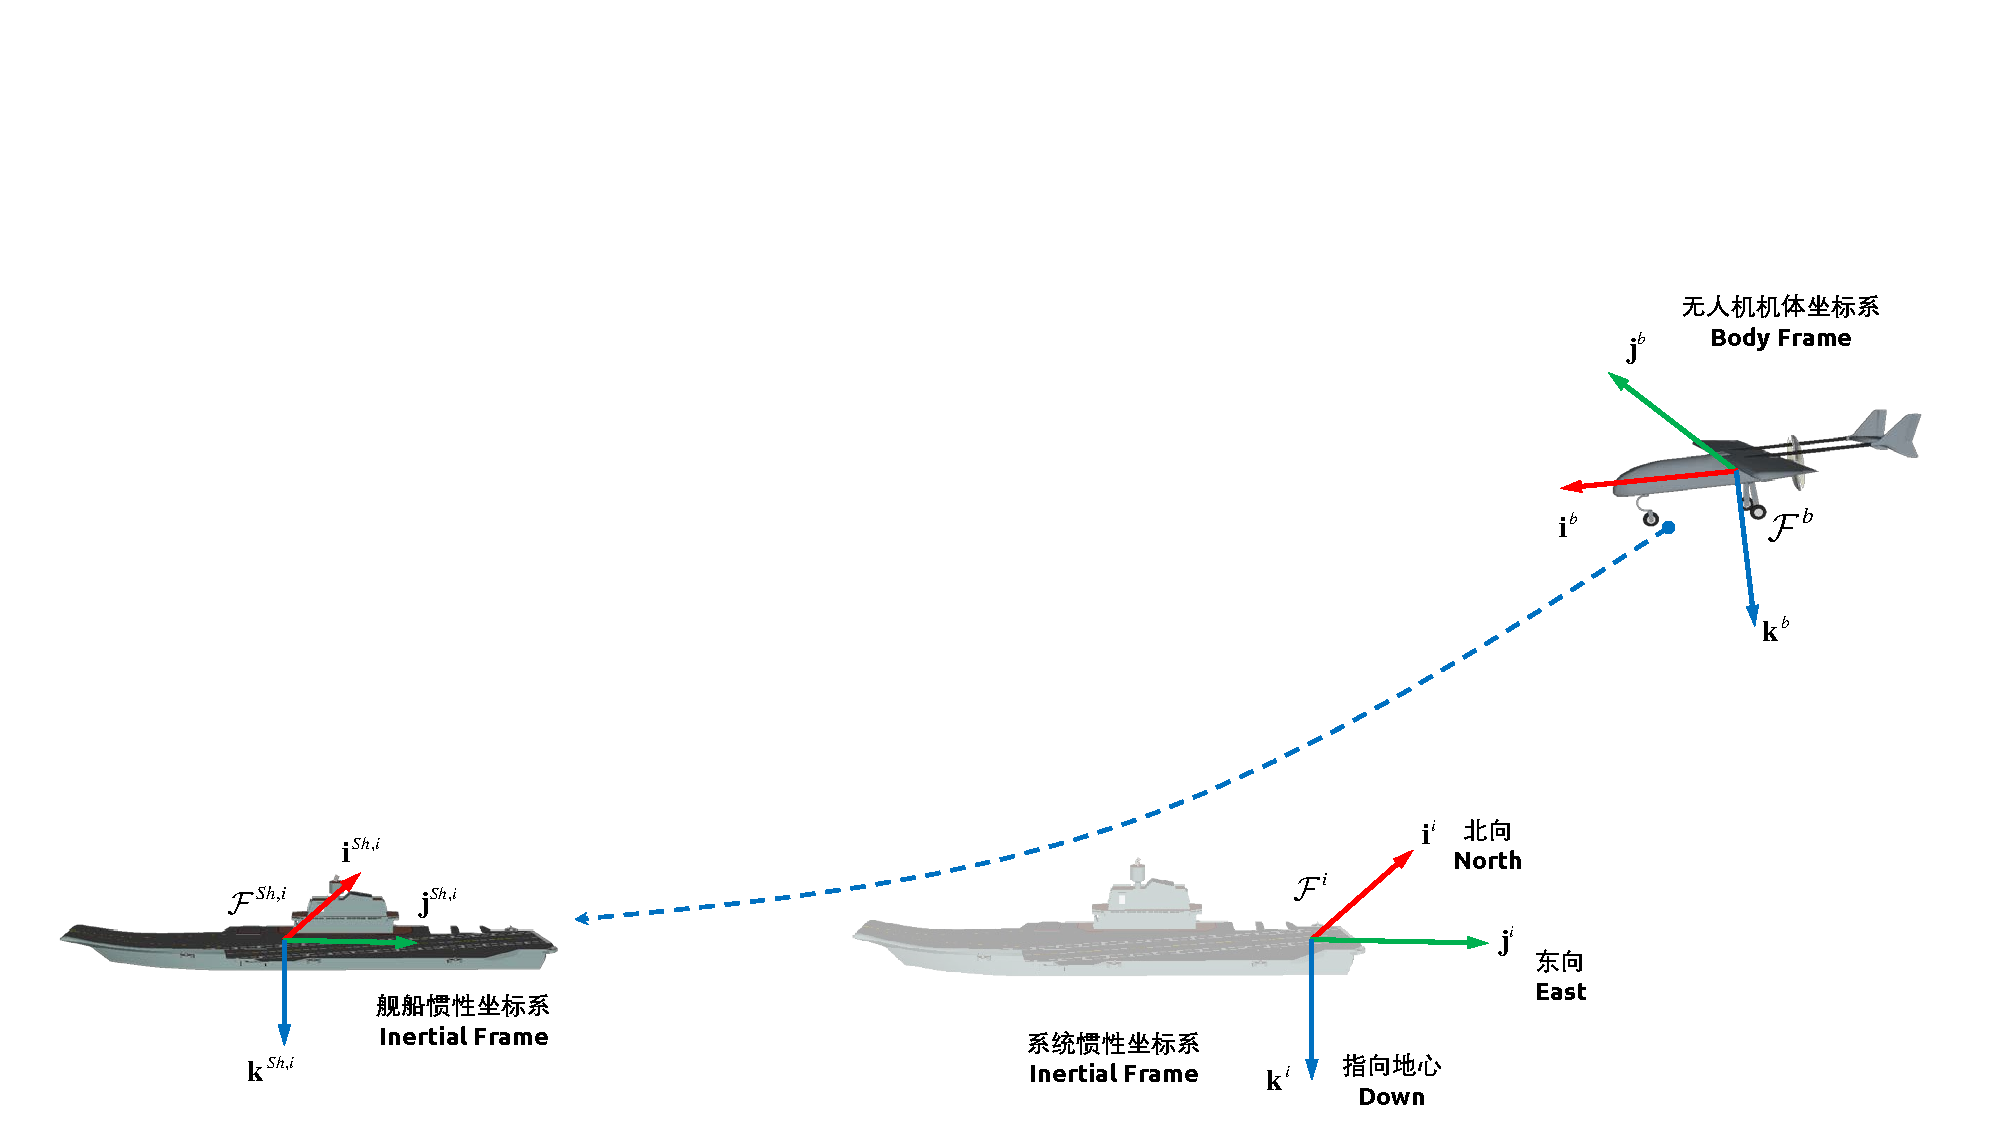
\includegraphics[width=\textwidth]{figs/chp02/chp02_01_sys_interial_frame.pdf}
	\caption{系统惯性坐标系}
	\label{fig:chp02_01_sys_interial_frame}
\end{figure}

\subsection{无人机惯性坐标系}
无人机惯性坐标系($\mathcal{F}^v$,Vehicle Inertial Frame),该坐标系的原点位于飞机的重心,三轴方向与系统坐标系平行。

\begin{figure}[htb]   
	\centering
	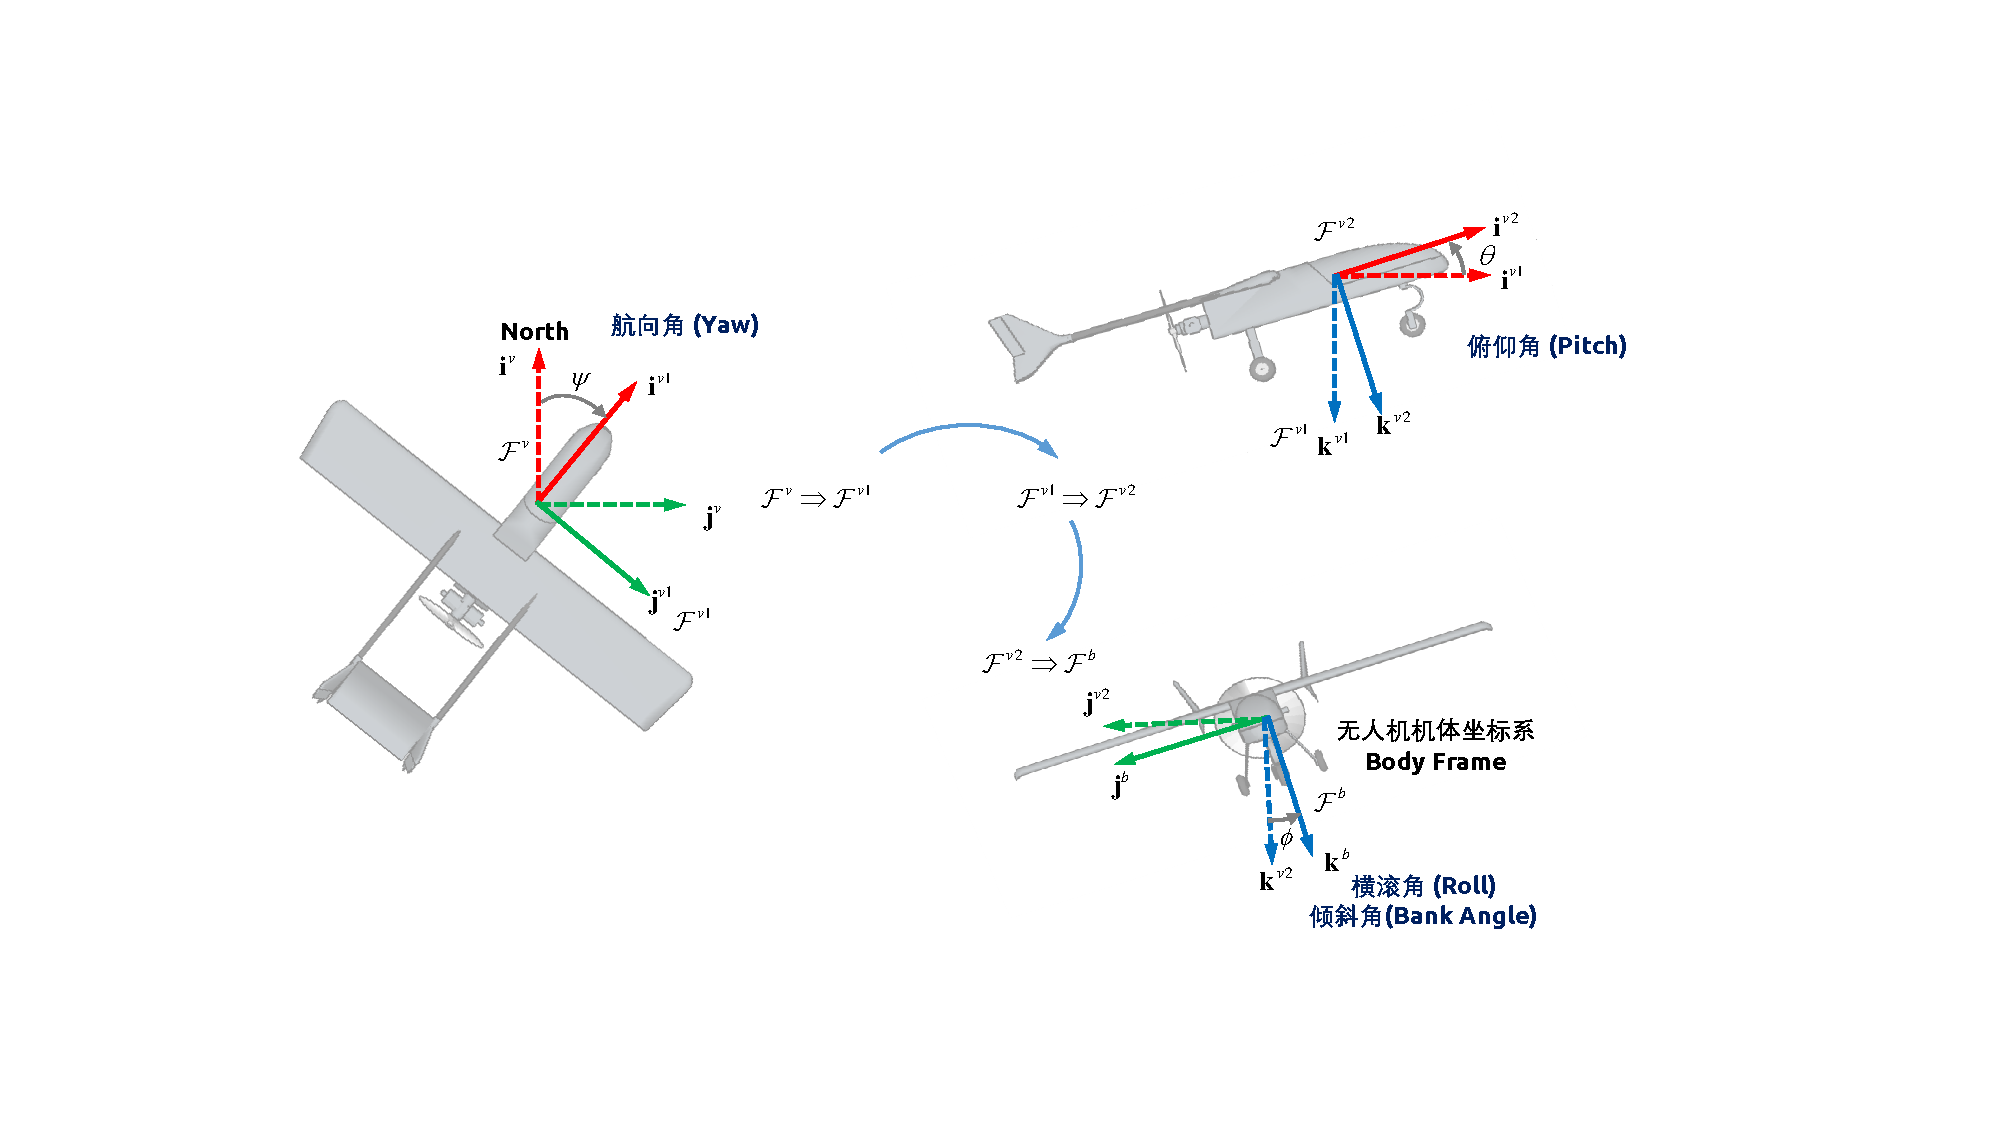
\includegraphics[width=\textwidth]{figs/chp02/chp02_02_uav_rpy.pdf}
	\caption{无人机机体坐标系与横滚角、俯仰角和偏航角定义}
	\label{fig:chp02_02_uav_rpy}
\end{figure}

无人机第一惯性辅助坐标系($\mathcal{F}^{v1}$ ),该坐标系绕无人机惯性坐标系$\mathbf{k}^v$轴按右手规则旋转得到,其中旋转角度定义为$\psi$,即偏航角(Yaw Angle)。

无人机第二惯性辅助坐标系($\mathcal{F}^{v2}$),该坐标系过绕人机第一惯性辅助坐标系$\mathbf{j}^{v1}$轴按右手规则旋转旋转得到,其旋转角度定义为$\theta$,即俯仰角(Pitch Angle)。

无人机机体坐标系($\mathcal{F}^b$,Body Frame ),该坐标系绕无人机第二惯性辅助坐标系$\mathbf{i}^{v2}$轴按右手规则旋转旋转得到,其旋转角度定义为$\phi$,即横滚角(Roll Angle),有时该角度也被称为倾斜角(Bank Angle)。上述四个坐标系之间的转换关系如图\ref{fig:chp02_02_uav_rpy}所示。

根据上述四个坐标系的几何关系,可以得到由机体惯性坐标系$\mathcal{F}^v$转换到机体坐标系$\mathcal{F}^b$的转换矩阵为
\begin{multline}
\mathcal{R}_v^b(\phi, \theta, \psi) =\mathcal{R}_{v2}^b(\phi)\mathcal{R}_{v1}^{v2}(\theta)\mathcal{R}_v^{v1}(\psi) \\
=\begin{bmatrix}
\cos \theta \cos \psi                             & \cos\theta \sin\psi                               & -\sin\theta         \\
-\cos\phi \sin\psi + \sin\phi \sin\theta \cos\psi & \cos\phi \cos\psi + \sin\phi \sin\theta\sin\psi   & \sin\phi \cos\theta \\
\sin\phi \sin\psi + \cos\phi \sin\theta \cos\psi  & -\sin\phi \cos\psi + \cos\phi \sin\theta \sin\psi & \cos\phi \cos\theta
\end{bmatrix}
\end{multline}


机体坐标系$\mathcal{F}^b$转换到稳定坐标系$\mathcal{F}^s$的转换矩阵为
\begin{equation} 
\mathcal{R}_b^s(\alpha) = \begin{bmatrix}
\cos \alpha                             & 0                               & \sin \alpha         \\
0 & 1   &0 \\
-\sin \alpha   & 0 & \cos \alpha
\end{bmatrix}
\end{equation}

稳定坐标系$\mathcal{F}^s$转换为风坐标系$\mathcal{F}^w$的转换矩阵为
\begin{equation} 
\mathcal{R}_s^w(\beta) = \begin{bmatrix} \sin \beta  & \cos \beta  &  0      \\  - \sin \beta & \cos \beta   &0 \\  0   & 0 &1  \end{bmatrix}
\end{equation}

风坐标系$\mathcal{F}^w$转换为机体坐标系$\mathcal{F}^b$转换矩阵为

\begin{equation} 
\mathcal{R}_w^b (\alpha,\beta) = \begin{bmatrix} \cos \beta \cos \alpha & - \sin \beta \cos \alpha  & - \sin \alpha      \\	 \sin \beta & \cos \beta   & 0 \\	\cos \beta   & -\sin \beta \sin \alpha & \cos \alpha \end{bmatrix}
\end{equation}

\subsection{无人机风向坐标系}
无人机风向坐标系($\mathcal{F}^w$,Wind Frame),该坐标系的$\mathbf{i}^w$轴与风速方向相同,可以通过旋转稳定坐标系的$\mathbf{k}^s$轴$\beta$角度得到,该角度$\beta$被定义为侧滑角。无人机攻角和侧滑角的定义如图\ref{fig:chp02_03_uav_aoa_bank}所示。
\begin{figure}[htb]   
	\centering
	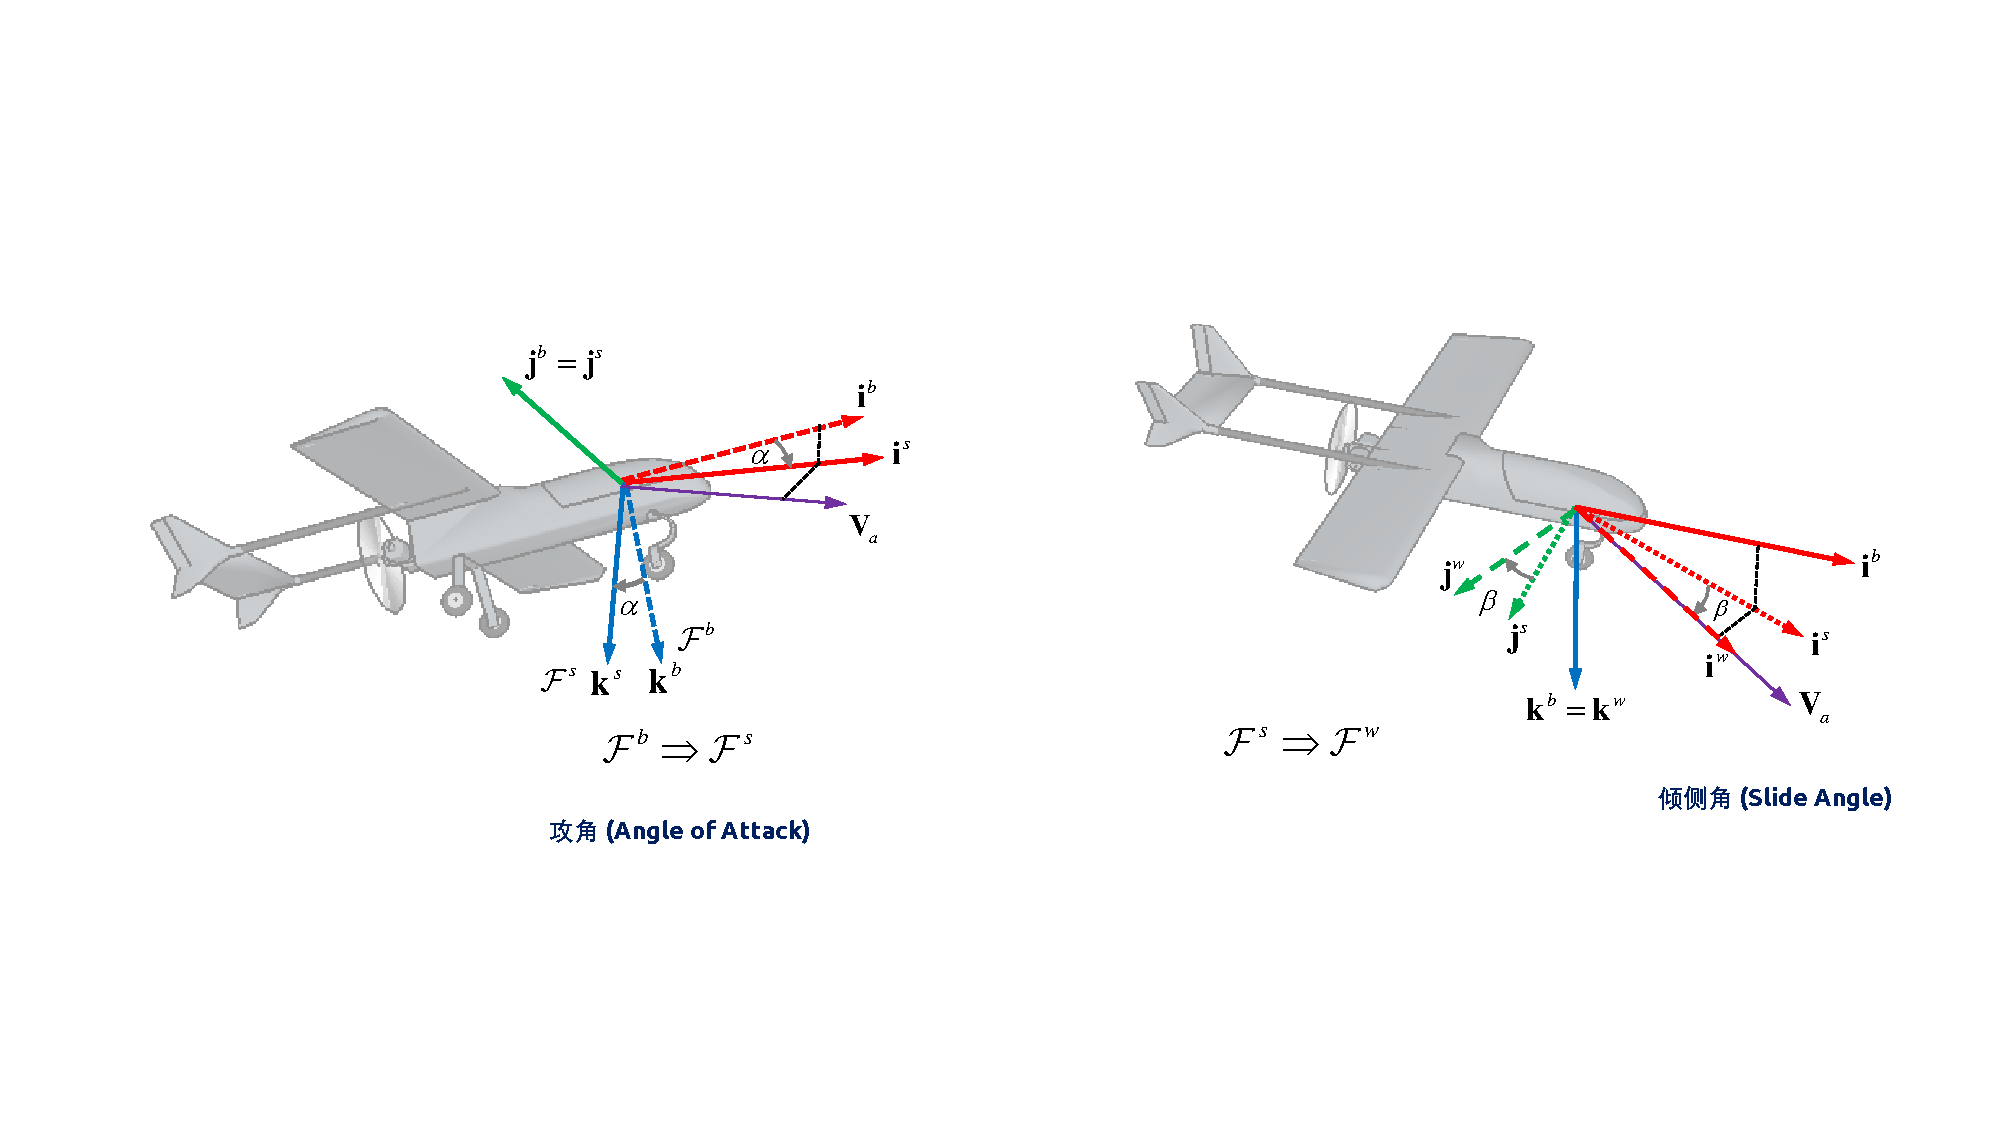
\includegraphics[width=\textwidth]{figs/chp02/chp02_03_uav_aoa_bank.pdf}
	\caption{无人机稳定坐标系与攻角、侧滑角定义}
	\label{fig:chp02_03_uav_aoa_bank}
\end{figure}

\subsection{无人机稳定坐标系}
无人机稳定坐标系($\mathcal{F}^s$,Stability Frame),该坐标系绕无人机机体坐标系$\mathbf{j}^b$按左手规则旋转得到,该坐标系表达如图\ref{fig:chp02_03_uav_aoa_bank}。其中,定义无人机相对于机体周边空气的速度向量为$\mathbf{V}_a$,其大小为$V_a$。为使机翼产生升力,机翼与风速的夹角必须为正,该角度定义为攻角。这里使用左手系的原因是为更方便的定义定义攻角$\alpha$的正负,即沿稳定坐标系$\mathbf{j^s}$按右手系转动到机体坐标系的角度为正。稳定坐标系的$\mathbf{i}^s$轴与空速向量$\mathbf{V}_a$在$\mathbf{i}^b$-$\mathbf{k}^b$的投影方向平行。

定义$\mathbf{V}_a$为空速(Airspeed),即无人机相对于周边流体的速度。
该向量在风坐标系$\mathcal{F}^w$的表达为
\begin{equation} 
\mathbf{V}_a^w=\begin{bmatrix} V_a \\ 0 \\ 0 \end{bmatrix}
\end{equation}
该向量在机体坐标系$\mathcal{F}^b$的表达为
\begin{equation} 
\mathbf{V}_a^b = \begin{bmatrix} u_r \\ v_r \\ w_r \end{bmatrix}
\end{equation}

$\mathbf{V}_g$定义为地速(Ground Speed),即无人机相对于系统惯性系的速度
无人机相对于惯性系的速度该向量在机体坐标系$\mathcal{F}^b$的表达为
\begin{equation}
\mathbf{V}_g^b=\begin{bmatrix} u \\ v \\w \end{bmatrix}
\end{equation}

$\mathbf{V}_w$定义为风速(Wind Speed),即风相对于系统惯性系的速度。
风速在机体坐标系$\mathcal{F}^b$的表达为
\begin{equation}
\mathbf{V}_w^b=\begin{bmatrix} u_w \\ v_w \\w_w \end{bmatrix} \\
=\mathcal{R}_v^b(\phi, \theta, \psi) \begin{bmatrix} w_n \\ w_e \\ w_d \end{bmatrix}
\end{equation}
其中$(w_n, w_e, w_d)$是风速在无人机惯性坐标系的表达。
上述三个速度直接的关系为
\begin{equation}
\mathbf{V}_a = \mathbf{V}_b - \mathbf{V}_w
\end{equation}

上述三个关系的表达如图\ref{fig:chp02_04_uav_wind_frame}所示,根据上述关系,可以得到风速在机体坐标系的另一个表达
\begin{equation}
\mathbf{V}_a^b  = \begin{bmatrix} u_r \\ v_r \\ w_r \end{bmatrix} =   \begin{bmatrix} u - u_w \\ v - v_w \\ w- w_w \end{bmatrix}
\end{equation}
根据风坐标系$\mathcal{F}^w$与$\mathcal{F}^b$机体坐标系的转换关系,风速在机体坐标系还可以表达为
\begin{equation}
\mathbf{V}_a^b  = \begin{bmatrix} u_r \\ v_r \\ w_r \end{bmatrix} \\
=  \mathcal{R}_w^b \begin{bmatrix} V_a \\ 0 \\ 0 \end{bmatrix} \\
=  \begin{bmatrix}	\cos \beta \cos \alpha & - \sin \beta \cos \alpha  & - \sin \alpha      \\	 \sin \beta & \cos \beta   & 0 \\ 	\cos \beta   & -\sin \beta \sin \alpha & \cos \alpha \end{bmatrix} \begin{bmatrix} V_a \\ 0 \\ 0 \end{bmatrix}
\end{equation}
由此可以得到上式更简便的表达
\begin{equation}
\begin{bmatrix} u_r \\ v_r \\ w_r \end{bmatrix}  = {V}_a \begin{bmatrix} \cos \alpha \cos \beta \\ \sin \beta  \\ \sin \alpha \cos \beta \end{bmatrix}
\end{equation}
注意,此处的$V_a$是风速向量的标量。

在已知风速相对于机体坐标系的向量表达时,可以进一步得到风速、攻角和侧滑角的计算
\begin{align}
V_a &= \sqrt{(u_r)^2+(v_r)^2+(w_r)^2} \\
\alpha &=  \tan^{-1}\frac{w_r}{u_r}  \\
\beta  &=  \sin^{-1} \big( \frac{u_r}{\sqrt{(u_r)^2+(v_r)^2+(w_r)^2}} \big)
\end{align}

\begin{figure}[htb]   
	\centering
	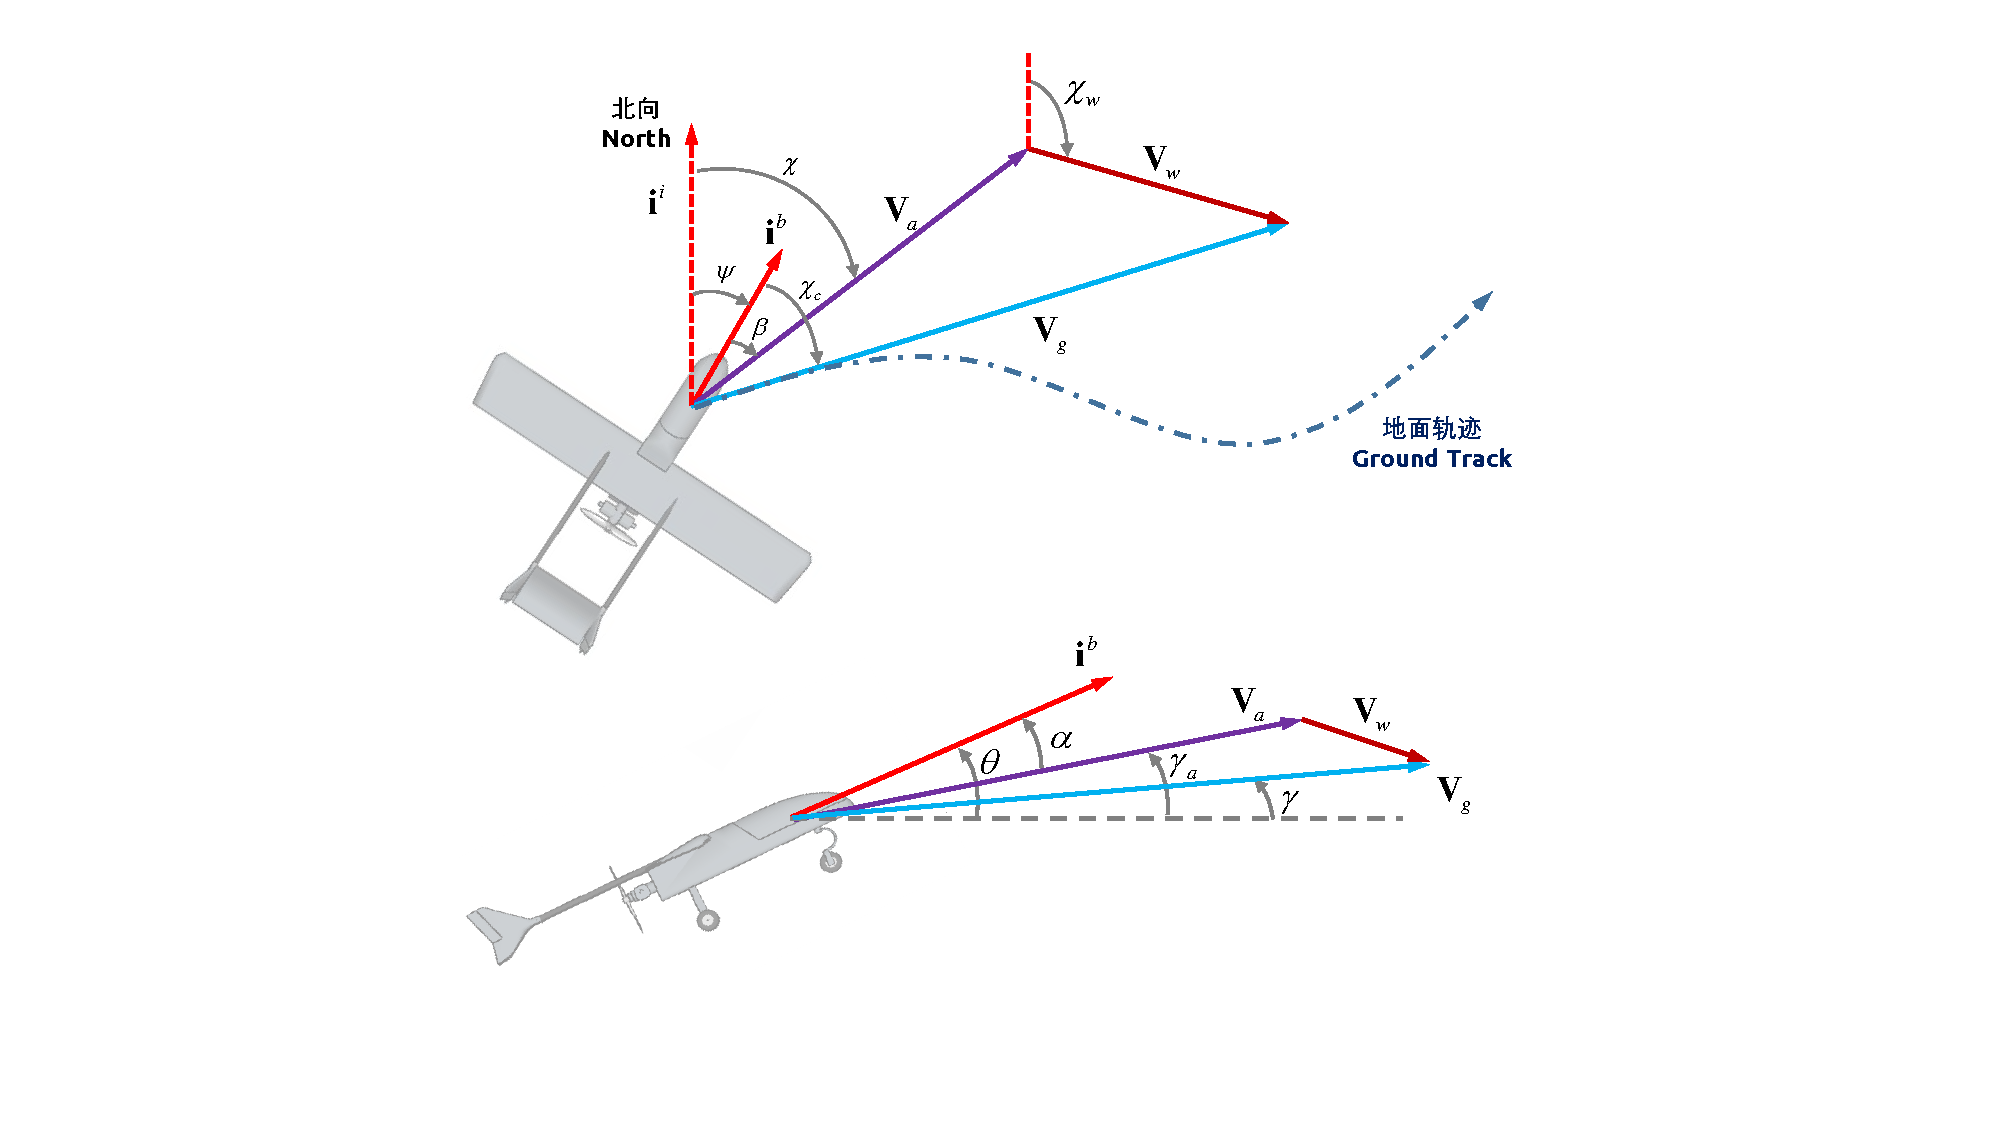
\includegraphics[width=0.8\textwidth]{figs/chp02/chp02_04_uav_wind_frame.pdf}
	\caption{无人机地速、风速和空速三角形}
	\label{fig:chp02_04_uav_wind_frame}
\end{figure}

 




\section{无人机系统运动学和动力学分析}
\subsection{三维空间向量微分}
假设在机体坐标系$\mathcal{F}^b$存在一个运动的向量$\mathbf{p}$,如图\ref{fig:chp02_06_vector_rotation}所示,该向量的数学表达为 
\begin{equation}
\mathbf{p }= p_x \mathbf{i}^b +  p_y \mathbf{j}^b +  p_z \mathbf{k}^b
\end{equation}
\begin{figure}[htb]   
	\centering
	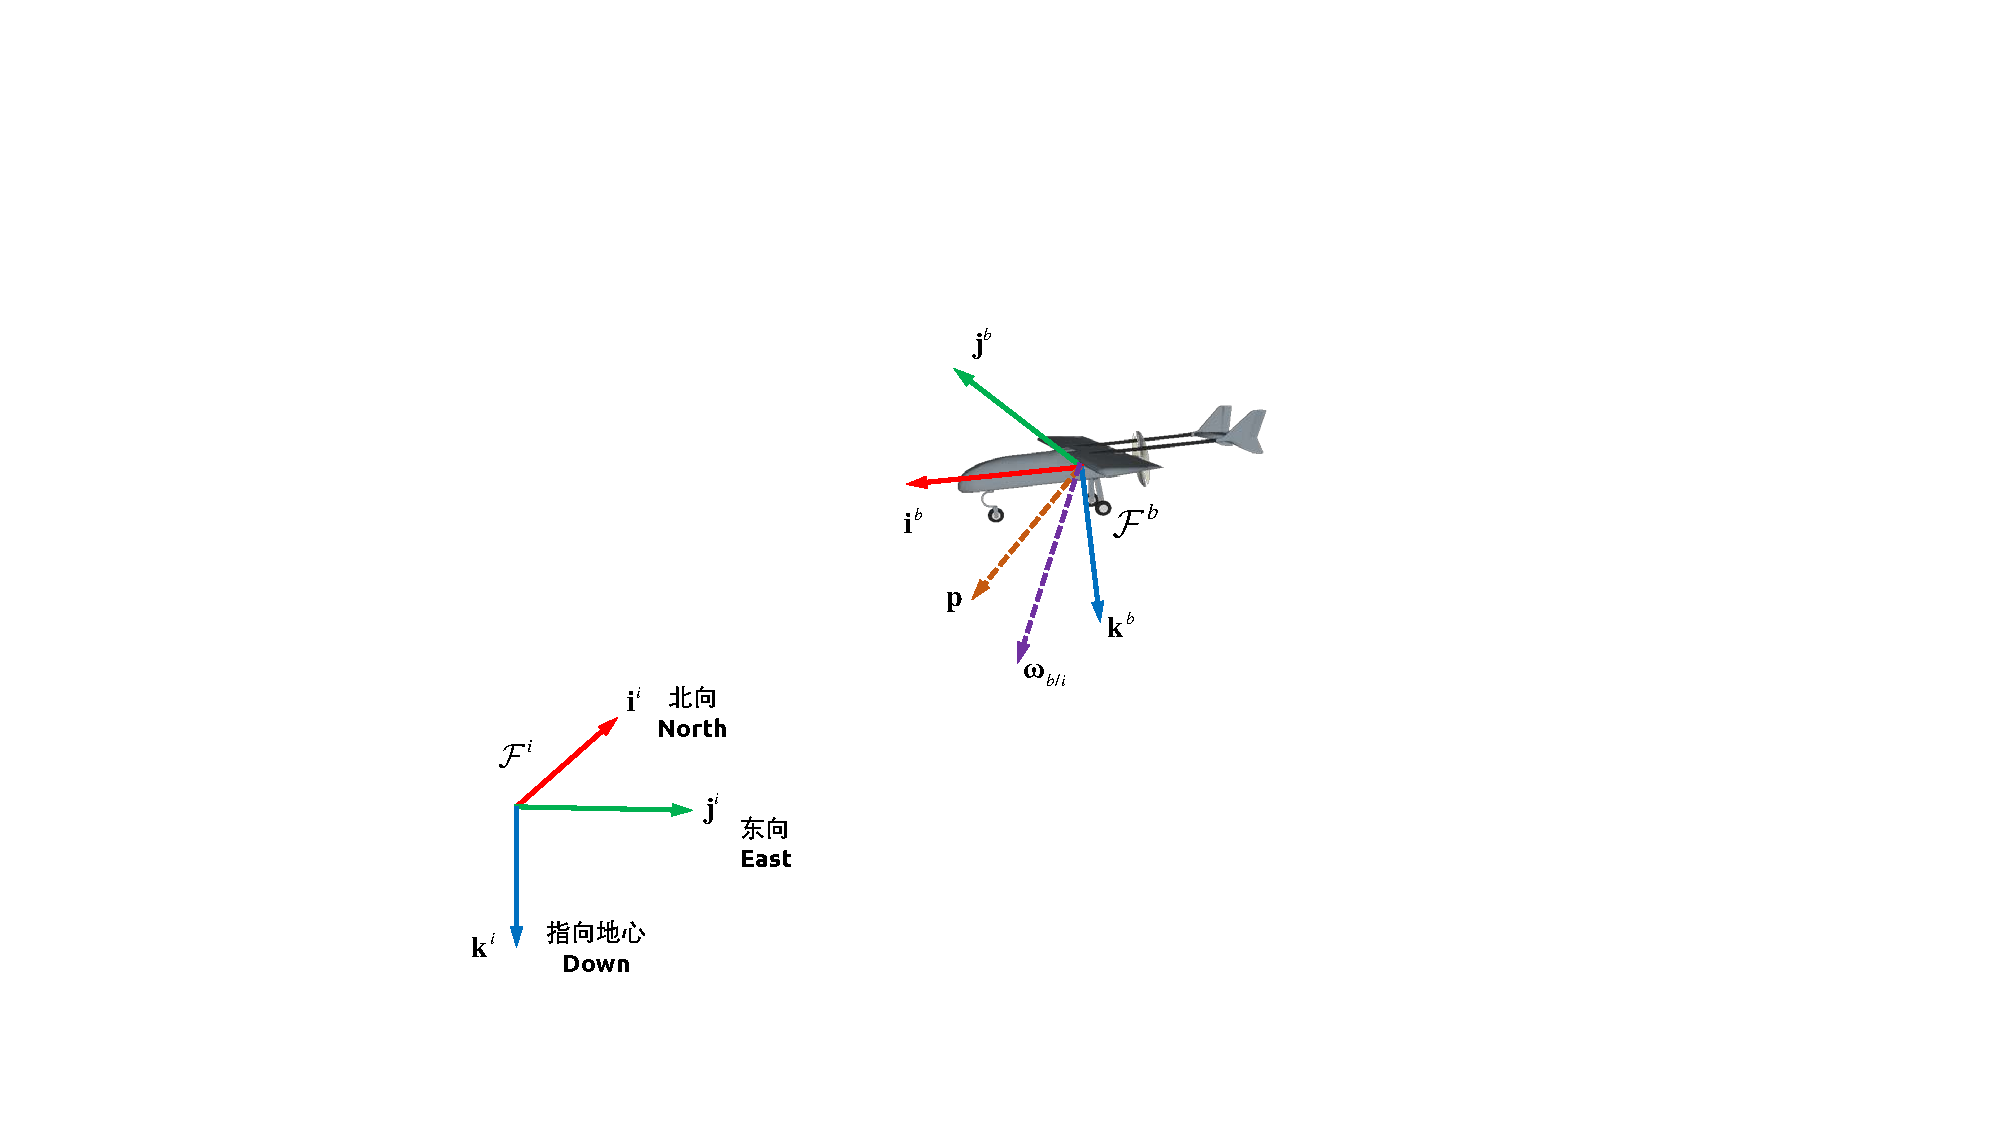
\includegraphics[width=0.8\textwidth]{figs/chp02/chp02_06_vector_rotation.pdf}
	\caption{三维空间向量微分}
	\label{fig:chp02_06_vector_rotation}
\end{figure}

此时机体坐标系$\mathcal{F}^b$与惯性坐标系$\mathcal{F}^i$只存绕转动向量$\mathbf{\omega}_{b/i}$的转动,不存在平动。由此得到该运动向量$\mathbf{p}$相对于系统坐标系$\mathcal{F}^i$的微分为
\begin{equation} \label{chp02_vector_derivative}
\frac{d}{dt_i} \mathbf{p} = \frac{d}{dt_b} \mathbf{p} + \mathbf{\omega}_{b/i} \times \mathbf{p}
\end{equation}
其中等式右侧的第一项具体表达为
\begin{equation}
\frac{d}{dt_i} \mathbf{p} = \dot{p}_x \mathbf{i}^b +  \dot{p}_y \mathbf{j}^b +  \dot{p}_z \mathbf{k}^b
\end{equation}
该部分可以通过设计无人机状态的观测器的获得。

\subsection{无人机空间位置定义}
因为飞机着舰过程的运动范围相对较小,由此对问题的坐标的整体构架主要选用Flat-Earth模型来替代WGS-84模型。首先,对于无人机在系统惯性系$\mathcal{F}^i$的位置定义为$(p_n\ p_e\ p_d)^T$,其中$n$, $e$  和$d$ 描述系统坐标系正北、正东和指向地心的方向。定义$h = -p_d$,用于描述无人机的飞行高度。无人机在系统惯性系的速度在机体坐标系$\mathcal{F}^b$的投影为$(u, v, w)$,无人机在机体坐标系$\mathcal{F}^b$的旋转角速度为$(p, q, r)$。则可以得到无人机速度在两个坐标系的相互转换关系
\begin{equation}
\frac{d}{dt} \begin{bmatrix} p_n \\ p_e \\ p_d \end{bmatrix}   =  (\mathcal{R}_v^b)^T \begin{bmatrix} u \\  v \\ w \end{bmatrix}  
\end{equation}
\begin{equation}
\resizebox{.9 \textwidth}{!} 
{ $
\begin{bmatrix} \dot{p}_n \\ \dot{p}_e \\ \dot{p}_d \end{bmatrix} = \begin{bmatrix}  cos \theta \cos \psi   &     -\cos\phi \sin\psi + \sin\phi \sin\theta \cos\psi                        &  \sin\phi \sin\psi + \cos\phi \sin\theta \cos\psi       \\
\cos\theta \sin\psi    & \cos\phi \cos\psi + \sin\phi \sin\theta\sin\psi   & -\sin\phi \cos\psi + \cos\phi \sin\theta \sin\psi \\
-\sin\theta  & \sin\phi \cos\theta & \cos\phi \cos\theta
\end{bmatrix} \begin{bmatrix} u \\  v \\ w \end{bmatrix}
$}
\end{equation}
进一步化解可以得到
\begin{align}
\begin{bmatrix} p \\ q \\ r \end{bmatrix}  &=   \begin{bmatrix}
1 &  0   & -\sin \theta      \\
0 &  \cos \phi  & \sin \phi \cos \theta \\	
0 & -\sin \phi   & \cos \phi \cos \theta
\end{bmatrix} \begin{bmatrix} \dot{\phi} \\ \dot{\theta} \\ \dot{\psi} \end{bmatrix} \\
\begin{bmatrix} \dot{\phi} \\ \dot{\theta} \\ \dot{\psi} \end{bmatrix}  &=  \begin{bmatrix}
1 &  \sin \phi \tan \theta  & - \cos \phi \tan \theta      \\
0 & \cos \phi   & -\sin \phi \\
0  & \sin \phi \sec \theta & \cos \phi \sec \theta
\end{bmatrix} \begin{bmatrix} p \\ q \\ r \end{bmatrix}
\end{align}

\subsection{无人机的外部力和力矩分析}
无人机的质量定义为$\mathsf{m}$,所受全部外力定义为$\mathbf{f}$,主要由重力$\mathbf{f}_g$、空气动力$\mathbf{f}_a$和电机拉力$\mathbf{f}_p$三部分组成
\begin{equation}
\mathbf{f} = \mathbf{f}_g + \mathbf{f}_a + \mathbf{f}_p
\end{equation}

重力在无人机惯性坐标系$\mathcal{F}^v$的表达为
\begin{equation}
\mathbf{f}_g^v = \begin{bmatrix}0  \\ 0  \\ \mathsf{m}g  \end{bmatrix}
\end{equation}

重力在无人机机体坐标系$\mathcal{F}^b$的表达为
\begin{equation}
\mathbf{f}_g^b =\mathcal{R}^b_v \begin{bmatrix}0  \\ 0  \\ \mathsf{m}g  \end{bmatrix} \\
= \begin{bmatrix} -\mathsf{m} g \sin \theta  \\ \mathsf{m}g \cos \theta \sin \phi  \\ \mathsf{m}g \cos\theta \cos \phi  \end{bmatrix}
\end{equation}

根据空气动力定义,在水平方向,无人机受到的升力$F_{lift}$、阻力$F_{drag}$和力矩$m$,其基本定义为
\begin{align}
F_{filt} = \frac{1}{2} V_a^2SC_L(\alpha, q, \delta_e) \\
F_{drag} = \frac{1}{2} V_a^2SC_D(\alpha, q, \delta_e) \\
m = \frac{1}{2} V_a^2ScC_m(\alpha, q, \delta_e)
\end{align}
其中$S$是机翼面积,$c$是机翼平均舷长,$C_L$、$C_D$和$C_m$是非线性空气动力参数。此外,无人机的控制面为三个,副翼偏移$\delta_a$,方向舵偏移$\delta_r$和升降舵偏移$\delta_e$。

根据本文目标无人机的空气特性,由此将上述气动力参数进一步展开为
\begin{align}
C_L(\alpha, q, \delta_e) &= C_X(\alpha) + {C_X}_q(\alpha) \frac{c}{2V_a}  q+ C_{X_{{\delta}_e}}(\alpha) \delta_e \\
C_D(\alpha, q, \delta_e) &= C_{Y_{0}} + C_{Y_{\beta}} \beta + C_{Y_r}(\alpha) \frac{b}{2V_a} r+ C_{Y_{\delta_\alpha}} \delta_\alpha +  C_{Y_{\delta_r}} \delta_r  \\ 
C_m(\alpha, q, \delta_e) &= C_Z(\alpha) + C_{Z_q}(\alpha) \frac{c}{2V_a}  q+ C_{Z_{\delta_e}} \delta_e
\end{align}
其中
\begin{align}
C_X(\alpha) &= -C_D(\alpha) \cos \alpha +  C_L(\alpha) \sin \alpha \\
C_{X_q}(\alpha) &= -C_{D_q} \cos \alpha +  C_{L_q} \sin \alpha \\
C_{X_{\delta_e}}(\alpha) &= -C_{D_{\delta_e}} \cos \alpha +  C_{L_{\delta_e}} \sin \alpha \\
C_Z(\alpha) &= -C_D(\alpha) \cos \alpha -  C_L(\alpha) \sin \alpha \\
C_X(\alpha) &= -C_{D_q} \sin \alpha -  C_{L_q} \cos \alpha \\
C_X(\alpha) &= -C_{D_{\delta_e}}  \sin \alpha -  C_{L_{\delta_e}} \cos \alpha \\
\end{align}
因为升力和阻力作用在无人机稳定坐标系$\mathcal{F}^s$上,因此将上述力转换到无人机的机体坐标系后,进一步得到
\begin{align}
\begin{bmatrix} f_x    \\ f_z  \end{bmatrix} = \begin{bmatrix}
\cos \alpha    & - \sin \alpha  \\
\sin \alpha       & \cos \alpha  \\
\end{bmatrix} \begin{bmatrix} -F_{drag}    \\ -F_{lift}  \end{bmatrix}
\end{align}
在竖直方向,无人机受到竖直方向的力和力矩为
\begin{align}
f_y = \frac{1}{2} \rho V_a^2 S C_y (\beta, p, r, \delta_a, \delta_r) \\
l  = \frac{1}{2} \rho V_a^2 S b  C_l (\beta, p, r, \delta_a, \delta_r) \\
n = \frac{1}{2} \rho V_a^2 S b C_n (\beta, p, r, \delta_a, \delta_r)
\end{align}
其中,$C_y$、$C_l$和$C_n$是非线性空气动力参数。

螺旋桨的推力建模为
\begin{equation}
\mathbf{f}_p = \frac{1}{2} \rho S_{prop} C_{prop}  \begin{bmatrix} (\mathsf{k}_{motor} \delta_t)^2 - V_a^2  \\ 0  \\ 0  \end{bmatrix}
\end{equation}
其中$\mathsf{k}_{motor}$是电机效率常数,$\delta_t$是电机的控制量,$S_{prop}$是螺旋桨的面积,$C_{prop}$是螺旋桨参数。

螺旋桨的力矩建模为
\begin{equation}
\mathbf{T}_p = -\mathsf{k}_{T_p} (\mathsf{k}_{\Omega} \delta_{t})^2
\end{equation}

其中$\Omega = \mathsf{k}_{\Omega} \delta_{t}$是螺旋桨的转速,$\mathsf{k}_{T_p}$是电机常数。

\subsection{无人机的平动分析}
对于无人机的平动,无人机的质量为$\mathsf{m}$和其受到的全部外力$\mathbf{f}$,根据顿第二定律可以得到
\begin{equation}
\mathsf{m} \frac{d \mathbf{V}_g}{d t_i} = \mathbf{f}
\end{equation}
代入\ref{chp02_vector_derivative}公式,可以得到
\begin{equation}
\mathsf{m}(\frac{d \mathbf{V}_g }{dt_b}+ \mathbf{\omega}_{b/i} \times \mathbf{V}_g)=\mathbf{f}
\end{equation}
同理,在机体坐标系$\mathcal{F}^b$可以得到
\begin{equation}
\mathsf{m}(\frac{d \mathbf{V}^b_g }{dt_b}+ \mathbf{\omega}_{b/i}^b \times \mathbf{V}^b_g)=\mathbf{f}^b
\end{equation}
其中$\mathbf{V}_g^b=(u, v, w)^T$描述无人机惯性系的速度向量在机体坐标系的表达,$\frac{d \mathbf{V}_g }{dt_b}=(\dot{u}, \dot{v}, \dot{w})^T$描述无人机速度在机体坐标系的变化率,$\mathbf{\omega}_{b/i}^b=(p, q, r)^T$描述无人机机体坐标系的转动角速度,$\mathbf{f}^b = (f_x, f_y, f_z)^T$描述外部合力向量在机体坐标系的表达。进一步可以得到
\begin{equation}
\begin{bmatrix} \dot{u} \\ \dot{v} \\ \dot{w}  \end{bmatrix} = \begin{bmatrix} rv-qw \\ pw-ru \\ qu-pv  \end{bmatrix} + \frac{1}{\mathsf{m}} \begin{bmatrix} f_x \\ f_y \\ f_z  \end{bmatrix}
\end{equation}



\subsection{无人机的转动分析}
对于无人机对转动,定义角动量$\mathbf{h}$和全部外力矩$\mathbf{m}$,由此可以得到
\begin{equation}
\frac{ d \mathbf{h}}{d t_i}=\mathbf{m}
\end{equation}
同理,对上式求在惯性系的微分
\begin{equation}
\frac{ d \mathbf{h}}{d t_i} = \frac{d\mathbf{h}}{dt_b} + \mathbf{\omega}_{b/i} \times \mathbf{h} = \mathbf{m}
\end{equation}
同理,在机体坐标系的表达为
\begin{equation}
\frac{ d \mathbf{h}^b}{d t_i} = \frac{d\mathbf{h}^b}{dt_b} + \mathbf{\omega}^b_{b/i} \times \mathbf{h}^b = \mathbf{m}^b
\end{equation}
对于刚体来说,角动量的表达通过惯量矩阵$\mathbf{J}$来定义
\begin{equation}
\mathbf{h}^b=\mathbf{J}  \mathbf{\omega}^b_{b/i}
\end{equation}
其中
\begin{align}
\mathbf{J} =\begin{bmatrix}	\int(y^2 + z^2)~d\mathsf{m} & -\int xy \ d\mathsf{m}        & -\int xz~d\mathsf{m} \\	-\int xy~d\mathsf{m}        & \int(x^2 + z^2)~d\mathsf{m} & -\int yz~d\mathsf{m} \\	-\int xz~d\mathsf{m}        & -\int yz~d\mathsf{m}  & \int(x^2 + y^2)~d\mathsf{m} \end{bmatrix}
\end{align}
根据无人机机体的对称性,该矩阵可以化简为
\begin{align}
\mathbf{J} = \begin{bmatrix}	J_x     & 0   & -J_{xz} \\	0       & J_y & 0       \\	-J_{xz} & 0   & J_z  \end{bmatrix}
\end{align}
改矩阵的逆为
\begin{align}
\mathbf{J}^{-1}=\frac{\mathrm{adj}(\mathbf{J}) }{\mathrm{det}(\mathbf{J}) } = \begin{bmatrix}	J_z / \Gamma     & 0   & J_{xz}/ \Gamma \\	0       & 1/ \Gamma & 0       \\	J_{xz}/ \Gamma & 0   & J_z/ \Gamma \end{bmatrix}
\end{align}
其中$ \Gamma = J_xJ_z - J_{xz}^2$ 。

同时,定义上式中的分量
\begin{align}
\dot{\mathbf{\omega}}^b_{b/i}=\frac{ d \mathbf{\omega}^b_{b/i}}{dt_b} = \begin{bmatrix} \dot{p} \\ \dot{q} \\ \dot{r}  \end{bmatrix}
\end{align}
该分量描述在机体坐标系角速度的变化率。

根据上述公式可以得到对角速度变化率的求解
\begin{equation}
\dot{\mathbf{\omega}}^b_{b/i} = \mathbf{J}^{-1}[{- \mathbf{\omega}}^b_{b/i} \times (\mathbf{J{\mathbf{\omega}}^b_{b/i}})+\mathbf{m}^b]
\end{equation}
定义无人机力矩在机体坐标系的表达$\mathbf{m}^b = (l, m, n)$

则可以得到对角速度变化率的进一步表达
\begin{equation}
\begin{bmatrix} \dot{p} \\ \dot{q} \\ \dot{r}  \end{bmatrix} =  \begin{bmatrix} \Gamma_1pq - \Gamma_2qr + \Gamma_3 l + \Gamma_4 n \\ \Gamma_5pr - \Gamma_6(p^2-r^2) + \frac{1}{Jy}m \\ \Gamma_7pq - \Gamma_1qr + \Gamma_4l + \Gamma_8 n  \end{bmatrix}
\end{equation}
其中各个分量的表达为
\begin{align}
\Gamma_1 &= \frac{J_{xz}(J_x-J_y+J_z)}{\Gamma}  \\
\Gamma_2 &= \frac{J_z(J_z-J_y) + J_{xz}^2}{\Gamma}  \\
\Gamma_3 &= \frac{J_z}{\Gamma}  \\
\Gamma_4 &= \frac{J_{xz}}{\Gamma}  \\
\Gamma_5 &= \frac{J_z - J_x}{J_y}  \\
\Gamma_6 &= \frac{J_{xz}}{J_y}  \\
\Gamma_7 &= \frac{(J_x-J_z)J_x+J_{xz}^2}{\Gamma}  \\
\Gamma_8 &= \frac{J_x}{\Gamma}  \\
\end{align}
 
\subsection{无人机运动轨迹数学描述}

\begin{figure}[htb]   
	\centering
	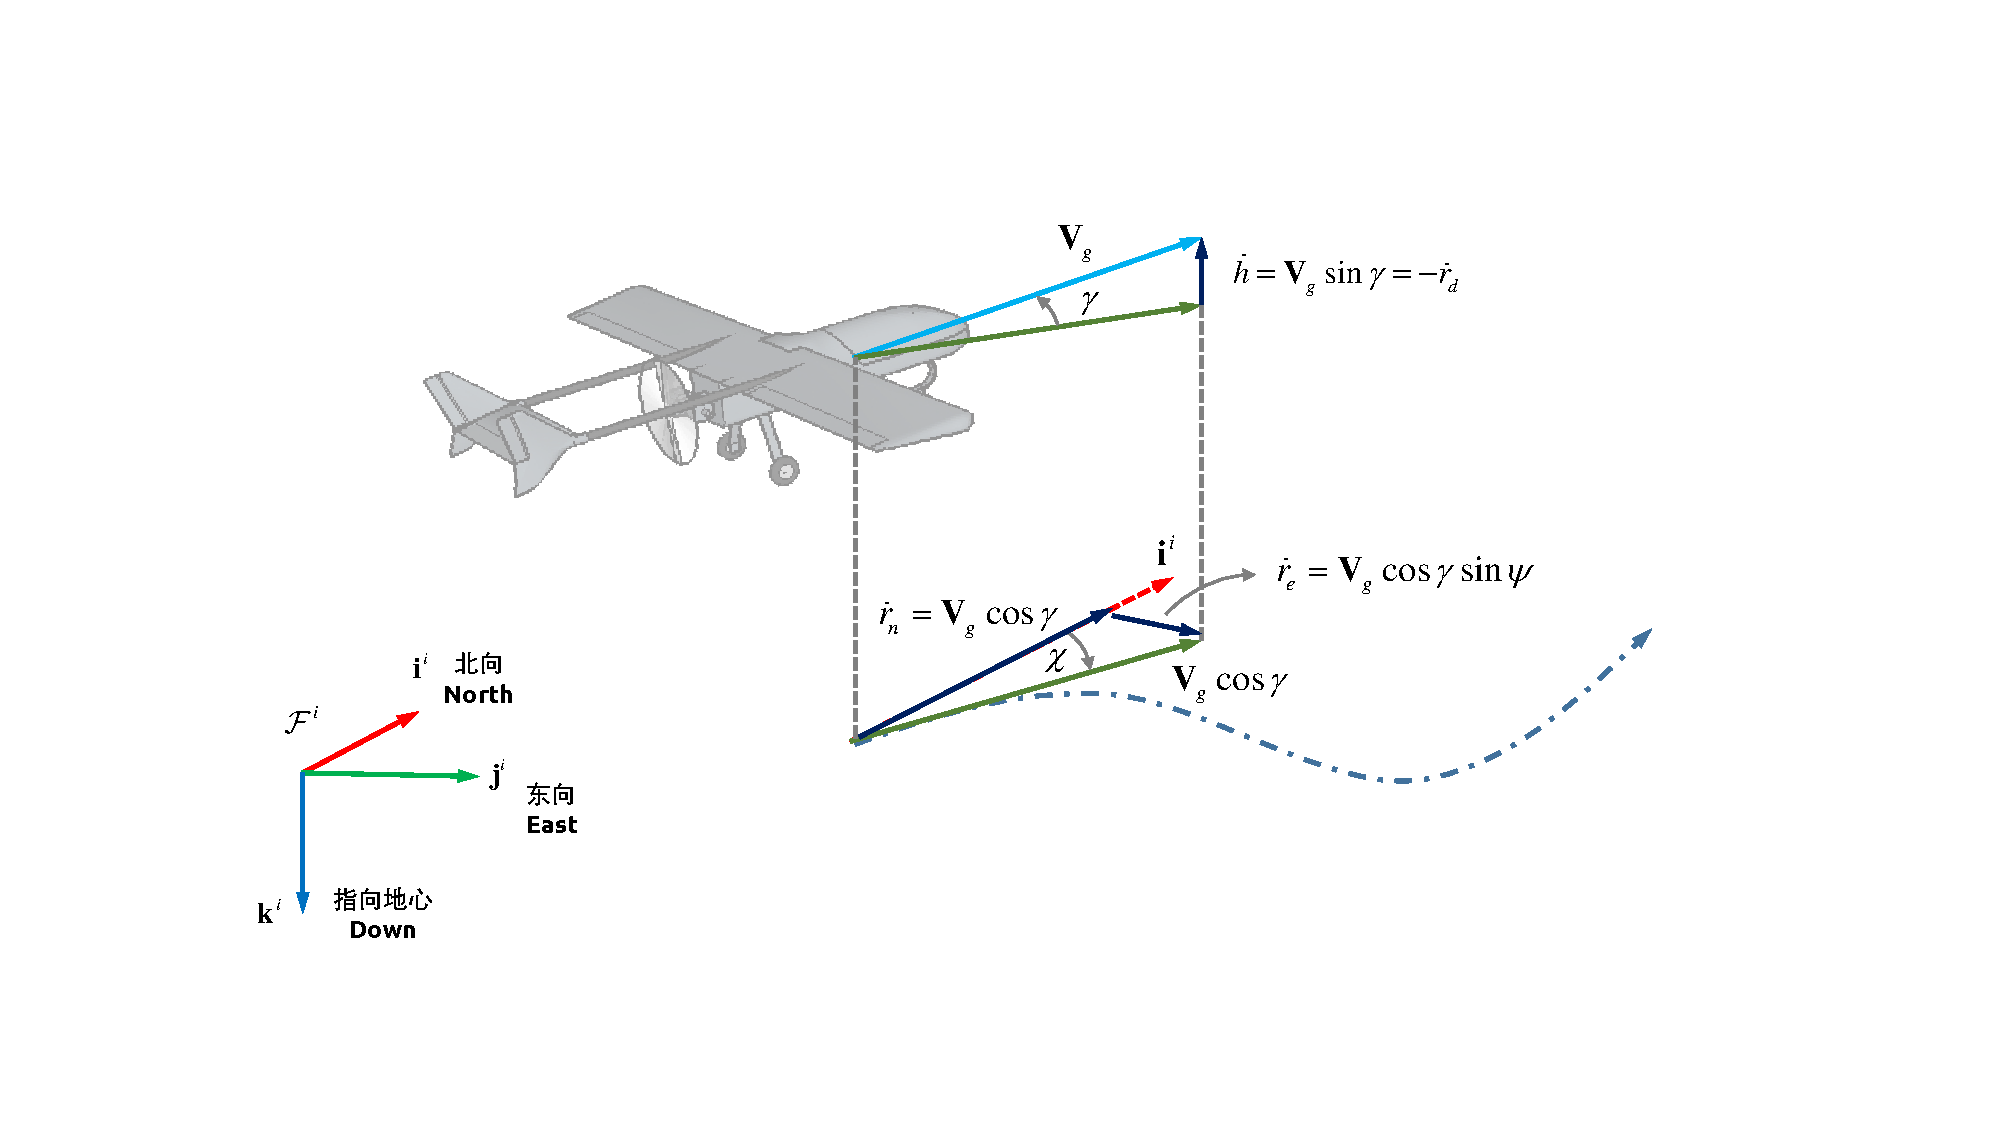
\includegraphics[width=0.8\textwidth]{figs/chp02/chp02_05_uav_course_frame.pdf}
	\caption{无人机运动轨迹描述}
	\label{fig:chp02_05_uav_course_frame}
\end{figure}

定义无人机在惯性系的坐标为$(p_n\ p_e\ p_d)^T$,无人机速度$\mathbf{V}_g$在惯性系的分量为$(\dot{p}_n\ \dot{p}_e\ \dot{p}_d)^T$,该速度的大小用$V_g = ||\mathbf{V}_g||$来表达,如图\ref{fig:chp02_05_uav_course_frame}所示。根据空间几何关系可以得到
\begin{equation}
\begin{bmatrix} \dot{p}_n \\\dot{p}_e \\ \dot{p}_d \end{bmatrix}  = {V}_g \begin{bmatrix} \cos \psi \cos \gamma \\ \sin \psi \cos \gamma  \\- \sin \gamma \end{bmatrix}
\end{equation}
其中航迹角$\gamma$定义为地速$\mathbf{V}_g$与惯性系北向$\mathbf{i}^i$与动向$\mathbf{j}^i$所构成的地平面的夹角,航迹偏航角$\chi$定义为地速$\mathbf{V}_g$在地面投影与正北方向的夹角。

由于无人机受到的升力为$F_{lift}$,在无人机进行协同转向(Coordinated Turn)时,根据力学关系可以得到横向和纵向公式
\begin{align}
&F_{lift} \sin \phi \cos (\chi - \psi) = \mathsf{m} \frac{v^2}{R}  \\
&F_{lift } \cos \phi = \mathsf{m} g \cos \gamma
\end{align}
将上述两式相除,并对$\chi$微分,可以得到
\begin{equation}
\dot{\chi} = \frac{g}{V_g} \tan \phi \cos (\chi - \psi)
\end{equation}
在没有风速影响下($V_g = V_a\ , \psi = \chi$),可以将上式进一步化简为
\begin{equation}
\dot{\psi} =\frac{g}{V_a} \tan \phi
\end{equation}
因为无人机的控制一般分为内环和外环,内环的控制速率较快,即飞行控制器可以很快使得无人机的姿态角收敛到指令期望位置,即$\gamma = \gamma^c\ , \phi = \phi^c$。因此,无人机的运动情况可以通过如下公式进一步描述
\begin{equation}
\begin{bmatrix} \dot{p}_n \\\dot{p}_e \\ \dot{p}_d \end{bmatrix}  = {V}_a \begin{bmatrix} \cos \psi \cos \gamma^c \\ \sin \psi \cos \gamma^c  \\- \sin \gamma^c \end{bmatrix} \\
\dot{\psi} =\frac{g}{V_a} \tan \phi^c
\end{equation}
由于无人机执行机构的物理约束,无人机的控制指令收到进一步约束
\begin{align}
|\phi^c| \le \bar{\phi} \\
|\gamma^c| \le \bar{\gamma}
\end{align}
其中$\bar{\phi}$和$\bar{\gamma}$为无人机系统的最大横滚角和下滑角约束。


\section{舰船系统坐标系定义}

舰船坐标系主要由舰船惯性坐标系、舰船龙骨坐标系和着舰点坐标系三部分组成。
\subsection{舰船惯性坐标系}
舰船惯性坐标系($\mathcal{F}^{Sh,i}$,Ship Inertial Frame),该坐标系的原点定义在舰船的中心位置,一般位于龙骨所在轴线,位于甲板下方。该坐标系的三个轴的方向分别与系统坐标系$\mathcal{F}^i$平行。该坐标系的表达如图\ref{fig:chp02_08_ship_interial_frame}所示。

\begin{figure}[htb]   
	\centering
	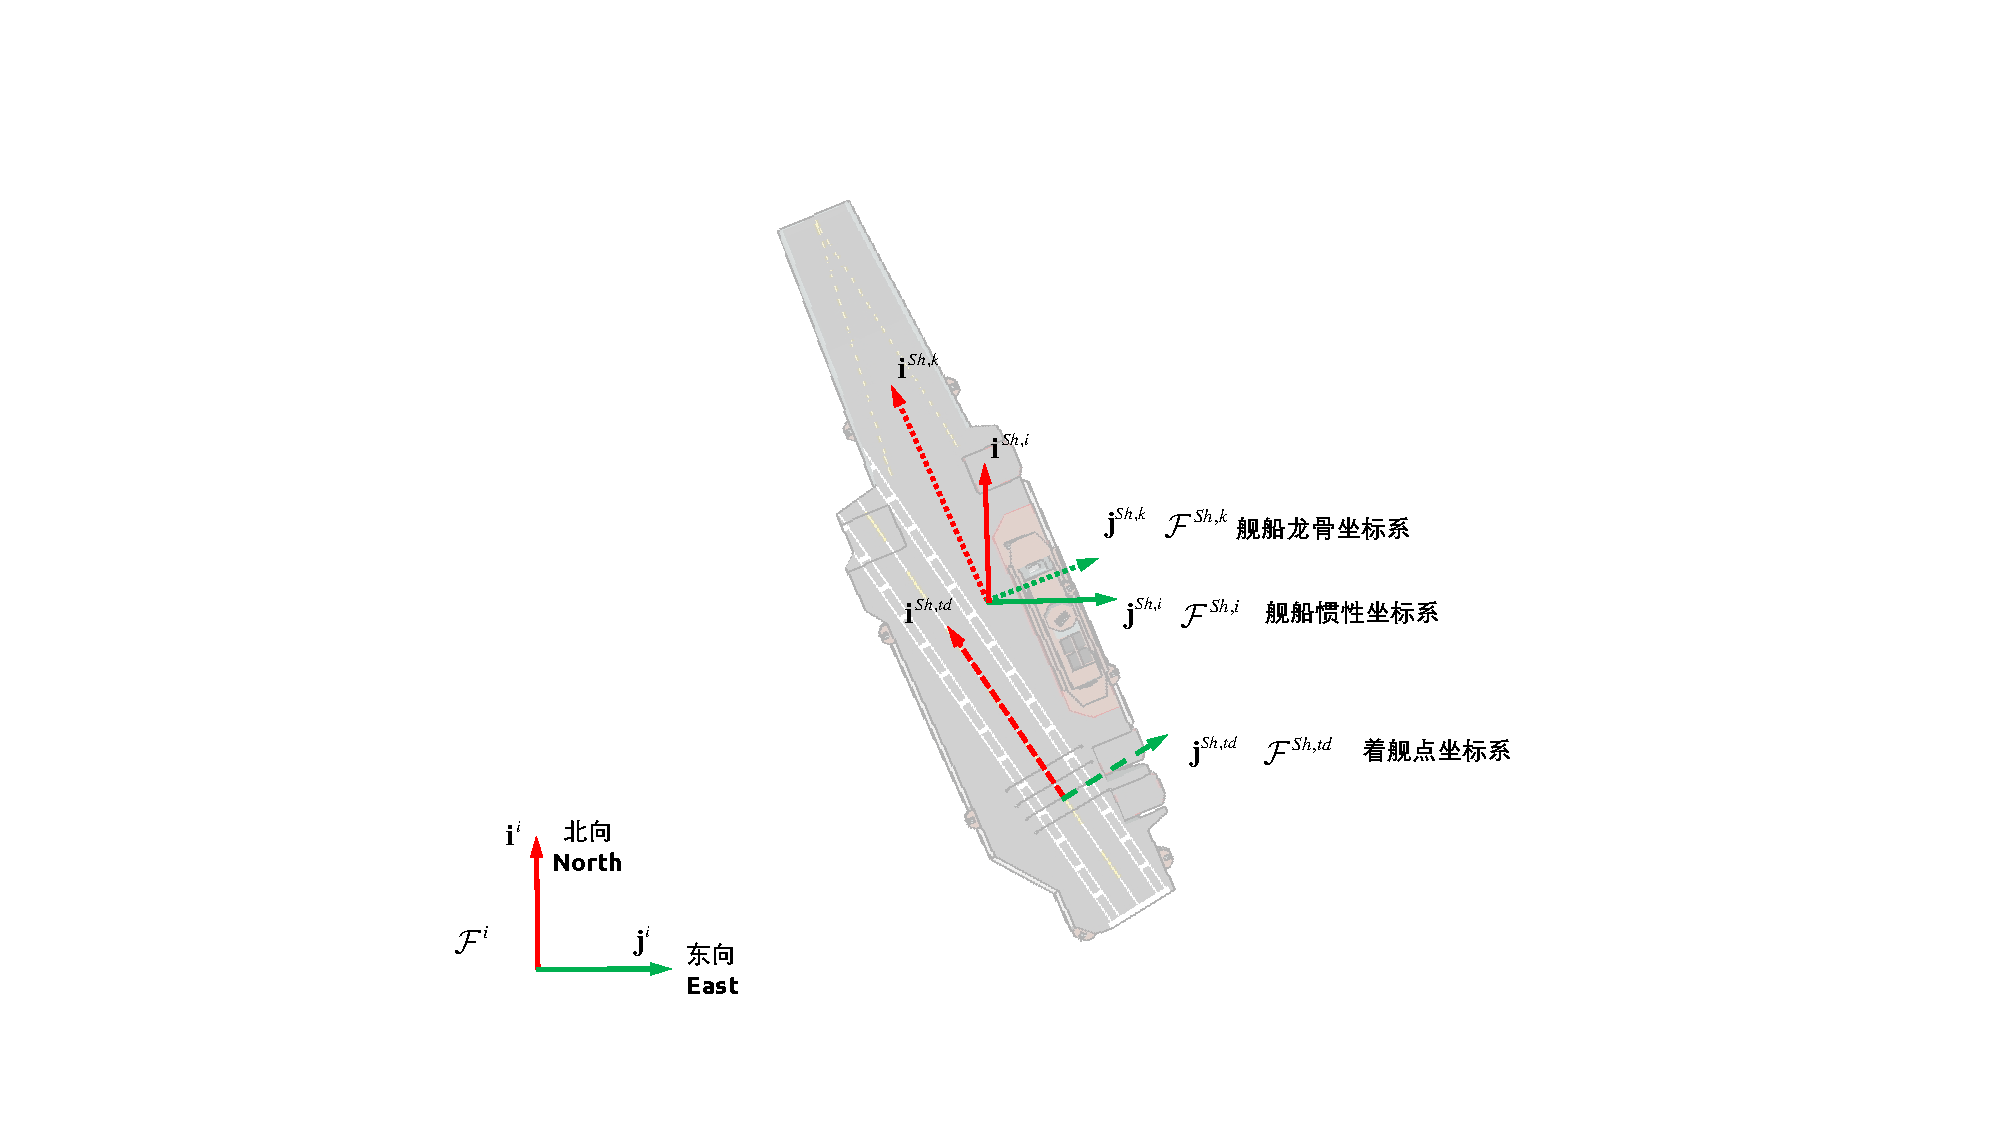
\includegraphics[width=0.8\textwidth]{figs/chp02/chp02_08_ship_interial_frame.pdf}
	\caption{舰船惯性坐标系}
	\label{fig:chp02_08_ship_interial_frame}
\end{figure}

\subsection{舰船龙骨坐标系}
舰船龙骨坐标系($\mathcal{F}^{Sh,k}$ ,Keel Frame),该坐标系的原点与舰船惯性坐标系相同,$\mathbf{i}^{Sh,k}$轴沿龙骨方向指向舰船前进方向,$\mathbf{j}^{Sh,k}$轴垂直于$\mathbf{i}^{Sh,k}$方向。因为该坐标系与船体固连,所以海浪的作用下,该坐标系随船体运动。与无人机机体坐标系类似,将舰船惯性坐标系按照3-2-1的顺序依次旋转至舰船龙骨坐标系,定义三次转动的角度为$\phi_{Sh}$、$\theta_{Sh}$和$\psi_{Sh}$,用于描述舰船的俯仰角、横滚角和偏航角。不同海况情况下,舰船龙骨坐标系还会存在周期性的扰动,由此定义$\Delta \phi_{Sh}$、$\Delta \theta_{Sh}$和$\Delta \psi_{Sh}$来描述舰船龙骨坐标系在俯仰、横滚和偏航三个轴线的扰动角度,定义$\Delta x_{surge}$、$\Delta y_{sway}$和$\Delta z_{heavy}$来描述三个坐标轴的位移偏差,即横摇、纵摇和沉浮。该坐标系的表达如图\ref{fig:chp02_09_ship_motion_frame}所示。

\begin{figure}[htb]   
	\centering
	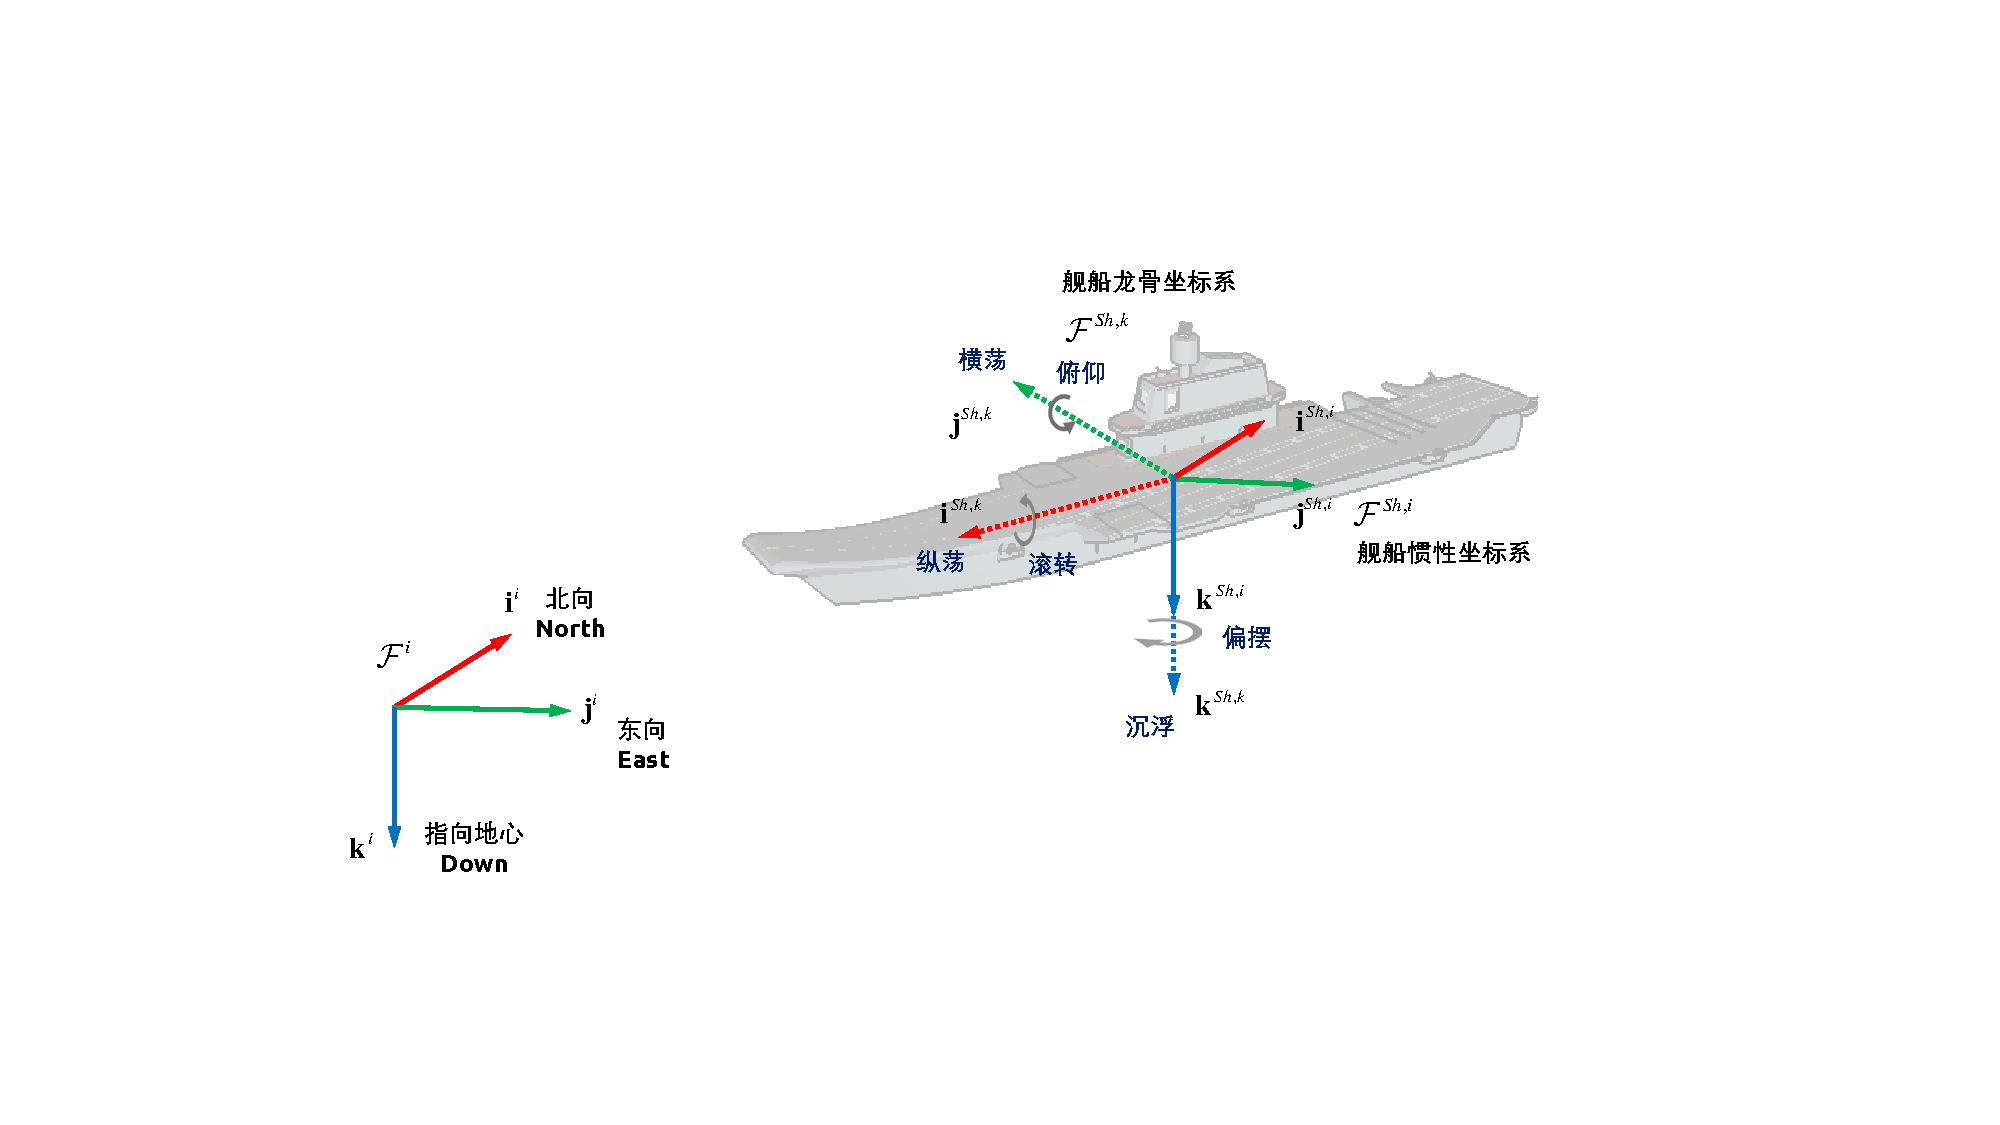
\includegraphics[width=\textwidth]{figs/chp02/chp02_09_ship_motion_frame.pdf}
	\caption{舰船系统坐标系的表达}
	\label{fig:chp02_09_ship_motion_frame}
\end{figure}


\subsection{着舰点坐标系}
着舰点坐标系($\mathcal{F}^{Sh,td}$,Touchdown Frame),该坐标系原点定义在第二条拦阻索的中间位置,$\mathbf{i}^{Sh,td}$轴沿降落跑道指向舰船运行前方,$\mathbf{j}^{Sh,td}$轴沿第二条拦阻索方向延长垂直于$\mathbf{i}^{Sh,td}$轴。

着舰点坐标系与舰船龙骨坐标系之间的转换关系定义为
\begin{equation}
\begin{bmatrix} x_{Sh,td} \\ y_{Sh,td} \\z_{Sh,td} \end{bmatrix} = \begin{bmatrix} x_{Sh,k} \\ y_{Sh,k} \\z_{Sh,k} \end{bmatrix} +\mathcal{R}_{Sh,k}^{Sh,td} \begin{bmatrix} \Delta x_{Sh,k}^{Sh,td} \\ \Delta y_{Sh,k}^{Sh,td} \\ \Delta z_{Sh,k}^{Sh,td} 
\end{bmatrix}
\end{equation}
其中$\Delta x_{Sh,k}^{Sh,td}$,$\Delta y_{Sh,k}^{Sh,td}$和$\Delta z_{Sh,k}^{Sh,td}$是着舰坐标系原点在舰船龙骨坐标系的坐标,$\mathcal{R}_{Sh,k}^{Sh,td}$是从舰船坐标系旋转到着舰点坐标系的旋转矩阵,该旋转矩阵的表达形式与无人机机体惯性坐标系转换到无人机机体坐标系的旋转矩阵相同,$(x_{Sh,k}\ y_{Sh,k}\ z_{Sh,k})$是舰船惯性坐标系上一点,该点在舰船着舰点坐标系上的坐标为$(x_{Sh,td}\ y_{Sh,td}\ z_{Sh,td})$。

\section{舰载引导系统坐标系定义}
由于舰船的运动,对于降落过程中的无人机需要提供有效的局部导航数据,本文设计的舰载引导系统坐标系主要用于描述引导系统对无人机的测量和导航。
\subsection{引导系统坐标系}
引导系统坐标系(Guidance Coordination System, $\mathcal{O}_c$)该坐标系的原点位于左侧引导系统的转台转轴的中心,$\mathbf{i}^{O,c}$轴指向右侧引导系统,并与着舰点坐标系的$\mathbf{j}^{Sh,td}$轴平行,$\mathbf{j}^{O,c}$轴与跑道纵向平行,指向远端无人机方向。该坐标系在舰船运动过程中与甲板固连,与期望着舰点坐标系的位置保持不变。一般而言,对于无人机着舰而言,期望着舰点的位置位于第一道和第二道拦阻索之间,靠近第二道拦阻索,如图\ref{fig:chp02_10_guidance_sys}所示;对于无人机装网回收而言,期望降落位置一般位于无人机回收网的几何中心。
\begin{figure}[htb]   
	\centering
	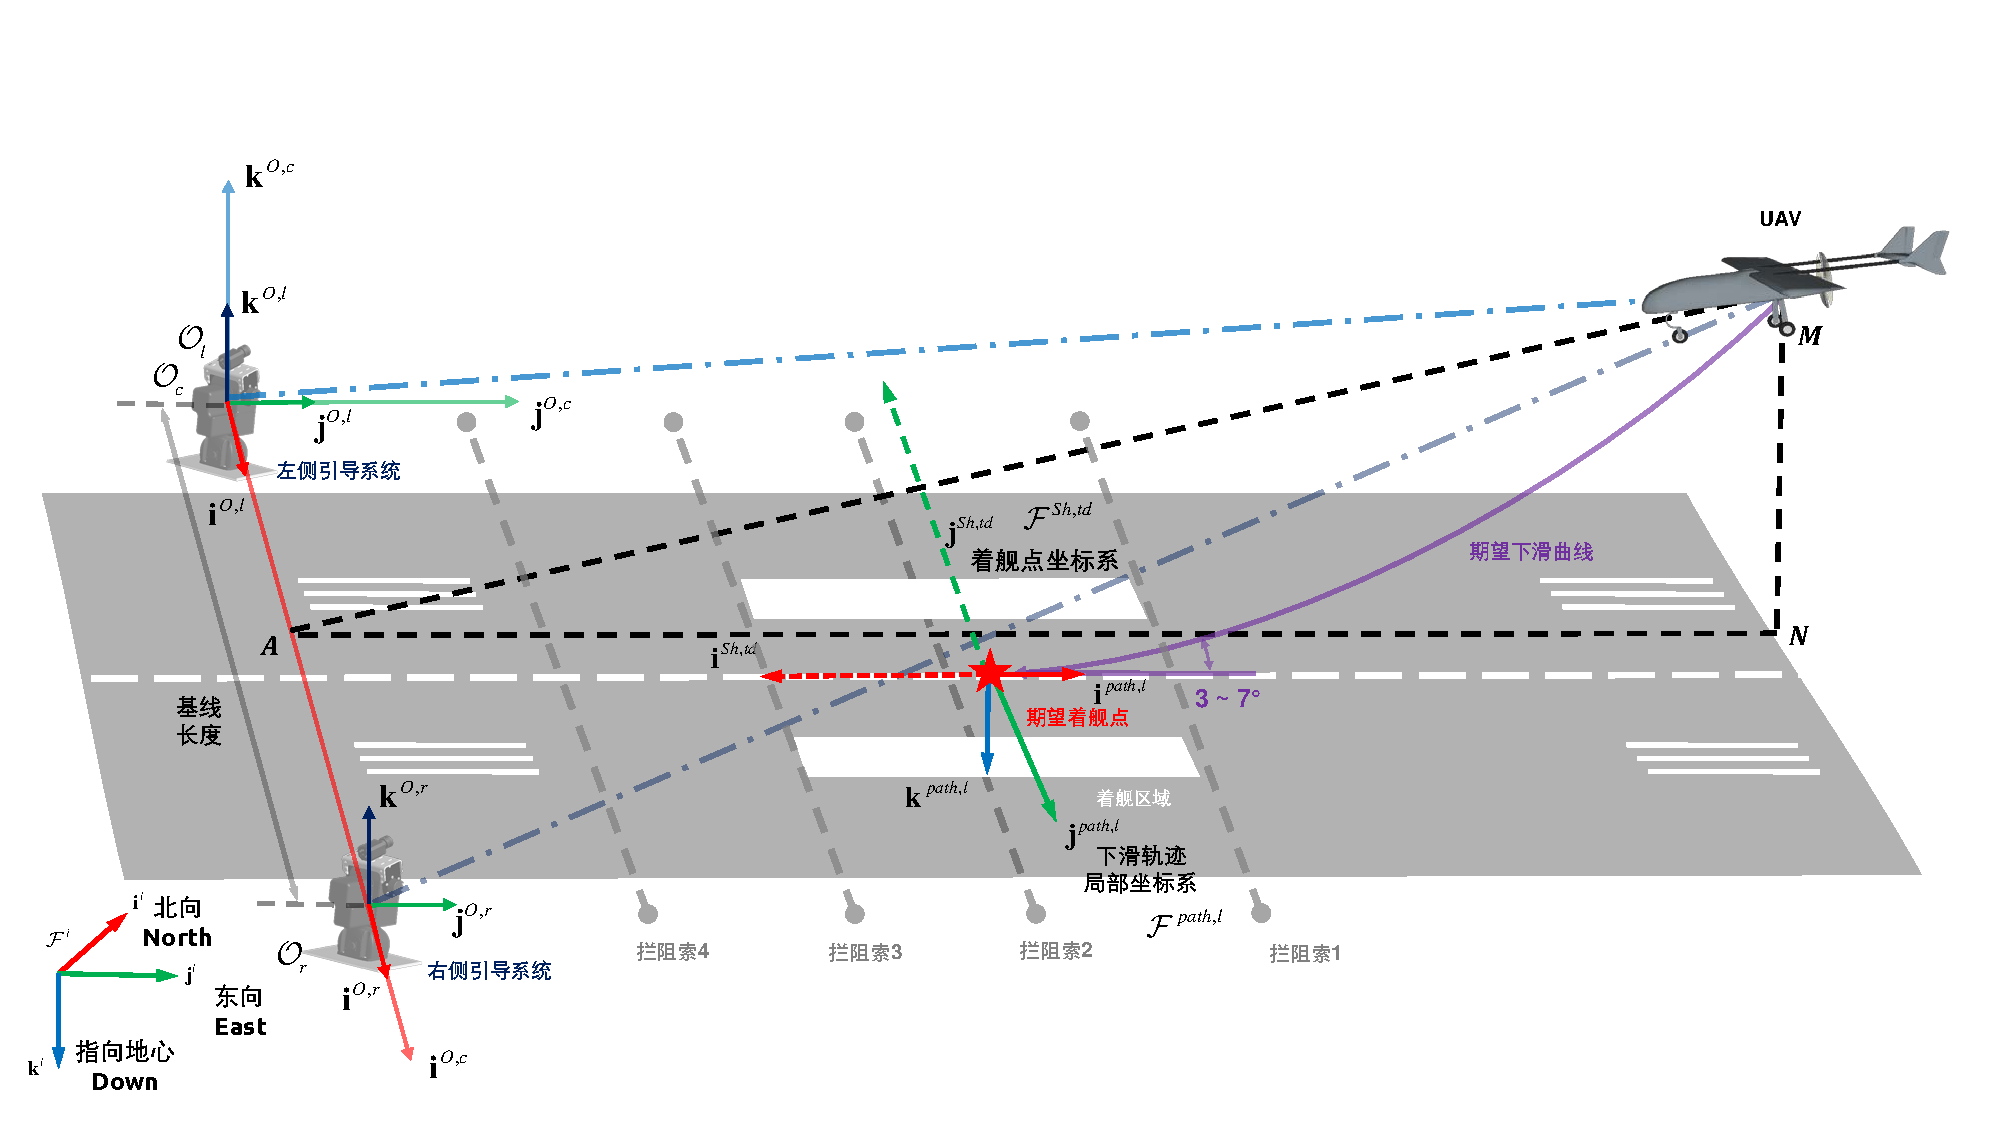
\includegraphics[width=\textwidth]{figs/chp02/chp02_10_guidance_sys.pdf}
	\caption{舰载引导系统相关坐标系}
	\label{fig:chp02_10_guidance_sys}
\end{figure}

\subsection{左右引导单元坐标系}
左侧引导系统坐标系($\mathcal{O}_l$)和右侧引导系统坐标系($\mathcal{O}_r$),这两个坐标系的原点别位于左侧和右侧引导系统的转台转轴中心,三个坐标轴的方向分别与光学引导系统相同。该引导单元坐标系也是用于立体解算无人机空间位置的主要坐标系。

\subsection{地心地固坐标系}
地心地固坐标系(Earth-Centered Earth-Fixed Coordinate System (ECEF),$\mathcal{O}_e$),该坐标系采用1984年\cite{WGS84}指定的地心空间右手坐标系(The World Geodetic System (WGS-84)),原点位于地球中心,$x$轴指向地球0°经线和0°纬线的交叉点,$y$轴指向地球的北极点。该坐标系通常用于大地测量、地图绘制和导航。本文后续试验中使用的该坐标系相关参数为 $R_{Ea}=6,378,137.0\ m$,$R_{Eb} = 6,356,752.0\ m$ ,$f=1/298.257223563$ 和 $e=0.08181919$。

\subsection{GPS坐标系}
GPS坐标系(The Geodetic Coordination System,$\mathcal{O}_g$)中的任意一点通常用$(\lambda\ \varphi\ h)$表示,其中 $\lambda$ 表示目标当前位置的经度, $\varphi$ 表示目标当前位置的纬度, $h$ 表示当前位置的高度。该数值一般通过GPS解算模块获得。

\subsection{GPS坐标系与地心地固坐标系之间的转换关系}
定义GPS经纬坐标系中任意一点$\mathbf{P}^g=(\lambda, \varphi, h)$,该点在地心地固坐标系的表达为

\begin{equation}
\textbf{P}^e
=
\left[\begin{array}{c}
X_e\\
Y_e\\
Z_e\\
\end{array}\right]
=
\left[\begin{array}{c}
(N_E+h)\cos \varphi \cos \lambda\\
(N_E+h)\cos \varphi \sin \lambda\\
(N_E(1-e^2)+h)\sin \varphi\\
\end{array}\right]
\end{equation}

其中$N_E$是基于当前纬度位置的参数,根据上文所述的相关参数,该数值通常通过下式进行计算。

\begin{equation}
N_E=\frac{R_{Ea}}{\sqrt{1-e^2 \sin^2 \varphi}}.
\end{equation}

\subsection{地心地固坐标系与系统惯性坐标系之间的转换关系}
定义系统惯性系原点在地心地固坐标系的原点为$\mathbf{P}_0^e(x_0\ y_0\ z_0)$,该点的GPS经纬坐标为$\mathbf{P}_0^g(\lambda_0\ \varphi_0\ h_0)$,地心坐标系中任意一点$\mathbf{P}^e$在系统惯性坐标系的表达为

\begin{equation}
\textbf{P}^i=\mathcal{R}_e^n(\textbf{P}^e - \textbf{P}_0^e)
\end{equation}

其中转换矩阵$\mathcal{R}_e^n$为

\begin{equation}
\mathcal{R}_e^n=\left[\begin{array}{ccc}
-\sin \varphi _{0} \cos \lambda _{0} & -\sin \varphi _{0} \sin \lambda _{0} & \cos \varphi _{0}  \\
-\sin \lambda _{0}           &           \cos \lambda _{0}            &          0           \\
-\cos \varphi _{0} \cos \lambda _{0} & -\cos \varphi _{0} \sin \lambda _{0} & -\sin \varphi _{0}
\end{array}\right]
\end{equation}

\subsection{舰船惯性坐标系与引导坐标系之间的转换关系}
定义在舰船惯性坐标系中的一点为$\mathbf{P}^{Sh,i}(X_{Sh,i}\ Y_{Sh,i}\ Z_{Sh,i})$,该点对应在引导坐标系的坐标为$\mathbf{P}^{c}(X_c\ Y_c\ Z_c)$,这两点之间的转换关系可以通过平移和旋转运算$(X_{Sh,i}, Y_{Sh,i}, Z_{Sh,i})\xrightarrow{\textbf{R}_{Sh,i}^c,T}(X_c, Y_c, Z_c) $得到,其矩阵表达形式为

\begin{equation}
\left[\begin{array}{c}
X_{Sh,i}\\
Y_{Sh,i}\\
Z_{Sh,i}\\
\end{array}\right]=\mathcal{R}_{Sh,i}^c
\left[\begin{array}{c}
X_{c}\\
Y_{c}\\
Z_{c}\\
\end{array}\right]+T_{Sh,i}^c
\end{equation}
其中
\begin{equation}
\mathcal{R}_{Sh,i}^c=\left[\begin{array}{ccc}
r_{11} & r_{12} & r_{13} \\
r_{21} & r_{22} & r_{23} \\
r_{31} & r_{32} & r_{33} 
\end{array}\right]
\ \ 
T_{Sh,i}^c=\left[\begin{array}{ccc}
t_{Sh,i}^c\\
t_{Sh,i}^c\\
t_{Sh,i}^c\\
\end{array}\right]
\end{equation}
理想情况下,舰船惯性坐标系与引导坐标系之间的几何关系可以通过定义旋转和平移量获得,但由于引导系统的安装误差,该矩阵通常通过外部标定方法得到。


​







%%% Local Variables:
%%% mode: latex
%%% TeX-master: "../main"
%%% End:

\begin{ack}

\end{ack}


%</thesis>
%    \end{macrocode}
%
% 在\LaTeX{}下管理参考文献将极其方便,建议使用Jabref生成条目,
% 用\verb|\cite|(其中\verb|upcite|是上标索引)索引即可。
% \verb|refs.bib|是你的参考文献名。
%    \begin{macrocode}
%<*thesis>
\cleardoublepage
\phantomsection
\addcontentsline{toc}{chapter}{参考文献}
\bibliographystyle{bstutf8}
\bibliography{ref/refs}

\begin{resume}

\section*{作者攻读博士学位期间发表的学术论文} % 发表的和录用的合在一起

[1] \textbf{Weiwei Kong}, Tianjiang Hu, Daibing Zhang, Lincheng Shen, and Jianwei Zhang. Localization Framework for Real-Time UAV Autonomous Landing: An On-Ground Deployed Visual Approach. Sensors 17, no. 6 (2017): 1437. (SCI检索,DOI:10.3390/\\s17061437)

[2] \textbf{Weiwei Kong}, Daibing Zhang, Xun Wang, Zhiwen Xian, and Jianwei Zhang. Autonomous landing of an UAV with a ground-based actuated infrared stereo vision system. In Intelligent Robots and Systems (IROS), 2013 IEEE/RSJ International Conference on, pp. 2963-2970. IEEE, 2013.(EI检索号:20140817338415)

[3] \textbf{Weiwei Kong}, Dianle Zhou, Yu Zhang, Daibing Zhang, Xun Wang, Boxin Zhao, Chengping Yan, Lincheng Shen, and Jianwei Zhang. A ground-based optical system for autonomous landing of a fixed wing UAV. In Intelligent Robots and Systems (IROS), 2014 IEEE/RSJ International Conference on, pp. 4797-4804. IEEE, 2014.(EI检索号:20144800250933)

[4] \textbf{Weiwei Kong}, Dianle Zhou, Daibing Zhang, and Jianwei Zhang. "Vision-based autonomous landing system for unmanned aerial vehicle: A survey." In Multisensor Fusion and Information Integration for Intelligent Systems (MFI), 2014 International Conference on, pp. 1-8. IEEE, 2014.(EI检索号:20150400443875)

[5] \textbf{Weiwei Kong}, Daibing Zhang, and Jianwei Zhang. A ground-based multi-sensor system for autonomous landing of a fixed wing UAV. In Robotics and Biomimetics (ROBIO), 2015 IEEE International Conference on, pp. 1303-1310. IEEE, 2015.(EI检索号:20161802327536)

[6] \textbf{Weiwei Kong}, Zhang Daibing, Zhao Shulong, Zhou Dianle, Zhao Boxin, Zhong Zhiwei, Ma Zhaowei, Tang Dengqing, and Zhang Jianwei. Autonomous track and land a MAV using a modified tracking-learning-detection framework. In Control Conference (CCC), 2015 34th Chinese, pp. 5359-5366. IEEE, 2015. (EI检索号:20154601538704)

[7] \textbf{孔维玮}, 先治文, 张代兵. 无人机垂直起降视觉自主导航系统的设计与实现[A]. 第九届全国信息获取与处理学术会议论文集 [C]. 2011年

[8] Bo Sun, \textbf{Weiwei Kong}, Junhao Xiao, and Jianwei Zhang. A hough transform based scan registration strategy for Mobile Robotic Mapping. In Robotics and Automation (ICRA), 2014 IEEE International Conference on, pp. 4612-4619. IEEE, 2014. 

[9] Tianjiang Hu, Boxin Zhao, Dengqing Tang, Daibing Zhang, \textbf{Weiwei Kong}, and Lincheng Shen. ROS-based ground stereo vision detection: implementation and experiments. Robotics and biomimetics 3, no. 1 (2016): 14.

[10] Yunyun Zhao, Xiangke Wang, \textbf{Weiwei Kong}, Lincheng Shen, and Shengde Jia. Decision-making of UAV for tracking moving target via information geometry. In Control Conference (CCC), 2016 35th Chinese, pp. 5611-5617. IEEE, 2016.

[11] Dengqing Tang, Tianjiang Hu, Lincheng Shen, Daibing Zhang, \textbf{Weiwei Kong}, and Kin Huat Low. Ground stereo vision-based navigation for autonomous take-off and landing of uavs: a chan-vese model approach. International Journal of Advanced Robotic Systems 13, no. 2 (2016): 67.

[12] Shulong Zhao, Xiangke Wang, \textbf{Weiwei Kong}, Daibing Zhang, and Lincheng Shen. A novel data-driven control for fixed-wing UAV path following. In Information and Automation, 2015 IEEE International Conference on, pp. 3051-3056. IEEE, 2015.

[13] Boxin Zhao, Tianjiang Hu, Yifeng Niu, Dengqing Tang, Zhaowei Ma, \textbf{Weiwei Kong}, and Lincheng Shen. Exploring the most appropriate feature detector and descriptor algorithm for on-board UAV image processing. In Information and Automation, 2015 IEEE International Conference on, pp. 56-61. IEEE, 2015.

[14] Hongliang Li, Zhiwei Zhong, \textbf{Weiwei Kong}, and Daibing Zhang. A fast calibration method for autonomous landing of UAV with ground-based multisensory fusion system. In Information and Automation, 2015 IEEE International Conference on, pp. 3068-3072. IEEE, 2015.

[15] 王勋, \textbf{孔维玮}, 张代兵, 朱华勇. 无人机跟踪地面非合作目标的分段引导与控制方法 [J]. 中国科学技术大学学报. 2012 (09)

\section*{作者攻读博士学位期间参加的课题研究} % 有就写,没有就删除

[1] 无人机XXXX着舰技术,装备预先研究项目,核心成员,2011年1月至2015年12月

[2] 无人机自主起降引导控制技术,军民融合协同创新研究项目,核心成员,2013年1月至2016年12月

[3] 机器人操作系统,学校重大应用基础研究项目,核心成员,2015年1月至2017年12月


%\section*{作者攻读博士学位期间撰写的项目报告} 
%[1] 无人机XXXX着舰技术技术报告,装备预先研究项目,2015年12月
%
%[2] 地基引导系统设计报告,军民融合协同创新项目,2016年2月
%
%[3] 控制系统设计报告,军民融合协同创新项目,2016年2月


\end{resume}

%</thesis>
%    \end{macrocode}
%
%<thesis>% 最后,需要的话还要生成附录,全文随之结束。
%    \begin{macrocode}
%<*thesis>
\appendix
\backmatter
% TeX
\chapter{模板提供的希腊字母命令列表}

大写希腊字母:
\begin{table}[htbp]
\centering
\begin{tabular}{llll}
\toprule
$\Gamma$~\verb|\Gamma| & $\Lambda$~\verb|\Lambda| & $\Sigma$~\verb|\Sigma| & $\Psi$~\verb|\Psi| \\
$\Delta$~\verb|\Delta| & $\Xi$~\verb|\Xi| & $\Upsilon$~\verb|\Upsilon| & $\Omega$~\verb|\Omega| \\
$\Theta$~\verb|\Theta| & $\Pi$~\verb|\Pi| & $\Phi$~\verb|\Phi| & \\
\midrule
$\varGamma$~\verb|\varGamma| & $\varLambda$~\verb|\varLambda| & $\varSigma$~\verb|\varSigma| & $\varPsi$~\verb|\varPsi| \\
$\varDelta$~\verb|\varDelta| & $\varXi$~\verb|\varXi| & $\varUpsilon$~\verb|\varUpsilon| & $\varOmega$~\verb|\varOmega| \\
$\varTheta$~\verb|\varTheta| & $\varPi$~\verb|\varPi| & $\varPhi$~\verb|\varPhi| & \\
\bottomrule
\end{tabular}
\end{table}

小写希腊字母:
\begin{table}[htbp]
\centering
\begin{tabular}{llll}
\toprule
$\alpha$~\verb|\alpha| & $\theta$~\verb|\theta| & $o$~\verb|o| & $\tau$~\verb|\tau| \\ 
$\beta$~\verb|\beta| & $\vartheta$~\verb|\vartheta| & $\pi$~\verb|\pi| & $\upsilon$~\verb|\upsilon| \\ 
$\gamma$~\verb|\gamma| & $\iota$~\verb|\iota| & $\varpi$~\verb|\varpi| & $\phi$~\verb|\phi| \\ 
$\delta$~\verb|\delta| & $\kappa$~\verb|\kappa| & $\rho$~\verb|\rho| & $\varphi$~\verb|\varphi| \\ 
$\epsilon$~\verb|\epsilon| & $\lambda$~\verb|\lambda| & $\varrho$~\verb|\varrho| & $\chi$~\verb|\chi| \\ 
$\varepsilon$~\verb|\varepsilon| & $\mu$~\verb|\mu| & $\sigma$~\verb|\sigma| & $\psi$~\verb|\psi| \\ 
$\zeta$~\verb|\zeta| & $\nu$~\verb|\nu| & $\varsigma$~\verb|\varsigma| & $\omega$~\verb|\omega| \\ 
$\eta$~\verb|\eta| & $\xi$~\verb|\xi| & $\varkappa$~\verb|\varkappa| & $\digamma$~\verb|\digamma| \\ 
\midrule
$\upalpha$~\verb|\upalpha| & $\uptheta$~\verb|\uptheta| & $\mathrm{o}$~\verb|\mathrm{o}| & $\uptau$~\verb|\uptau| \\ 
$\upbeta$~\verb|\upbeta| & $\upvartheta$~\verb|\upvartheta| & $\uppi$~\verb|\uppi| & $\upupsilon$~\verb|\upupsilon| \\ 
$\upgamma$~\verb|\upgamma| & $\upiota$~\verb|\upiota| & $\upvarpi$~\verb|\upvarpi| & $\upphi$~\verb|\upphi| \\ 
$\updelta$~\verb|\updelta| & $\upkappa$~\verb|\upkappa| & $\uprho$~\verb|\uprho| & $\upvarphi$~\verb|\upvarphi| \\ 
$\upepsilon$~\verb|\upepsilon| & $\uplambda$~\verb|\uplambda| & $\upvarrho$~\verb|\upvarrho| & $\upchi$~\verb|\upchi| \\ 
$\upvarepsilon$~\verb|\upvarepsilon| & $\upmu$~\verb|\upmu| & $\upsigma$~\verb|\upsigma| & $\uppsi$~\verb|\uppsi| \\ 
$\upzeta$~\verb|\upzeta| & $\upnu$~\verb|\upnu| & $\upvarsigma$~\verb|\upvarsigma| & $\upomega$~\verb|\upomega| \\ 
$\upeta$~\verb|\upeta| & $\upxi$~\verb|\upxi| & & \\ 
\bottomrule
\end{tabular}
\end{table}

希腊字母属于数学符号类别,请用\verb|\bm|命令加粗,其余向量、矩阵可用\verb|\mathbf|。


\end{document}
%</thesis>
%    \end{macrocode}
%
% 当然还有一些收尾工作,校验审阅自不必说。接下来你需要:修改论文中英文日期,
% 生成盲评,生成明(盲)评A3封面。
%
% {\color{blue}Happy \TeX{}ing! 欢迎提各式各样的意见!}
%
% \newpage\relax%
%
% \StopEventually{\PrintChanges}
% \clearpage
%
% \section{实现细节}
% 我们首先介绍文档模板的基本信息以及宏包和配置,
% 然后依照国防科学技术大学论文模板的书写规范一节一节的介绍实现步骤。
%
% \changes{v1.2}{2009/09/28}{添加了A3封面制作}
%
% \subsection{基本信息}
%    \begin{macrocode}
%<cls>\NeedsTeXFormat{LaTeX2e}[1999/12/01]
%<cls>\ProvidesClass{nudtpaper}
%<cfg>\ProvidesFile{nudtpaper.cfg}
%<cls|cfg>[2011/07/17 v2.2 NUDT paper template]
%    \end{macrocode}
%
% \subsection{宏包配置}
%
%<*cls>
%
%\changes{v0.99}{2009/08/17}{add package options}
% 当前的宏包选项在之前已经介绍了,下面是实现步骤,就是几个\verb|if|。
%\changes{v1.6}{2009/12/01}{添加单独的单双面控制}
%\changes{v2.0}{2010/11/09}{添加盲评控制}
%
%    \begin{macrocode}
\newif\ifismaster\ismastertrue
\DeclareOption{master}{\ismastertrue}
\DeclareOption{doctor}{\ismasterfalse}
\newif\ifisanon\isanonfalse
\DeclareOption{anon}{\isanontrue}
\newif\ifistwoside\istwosidefalse
\DeclareOption{twoside}{\istwosidetrue}
\DeclareOption*{\PackageWarning{nudtpaper}{Unknown Option '\CurrentOption'}}
% handle fonts
\newif\ifisttf\isttffalse
\newif\ifisotf\isotffalse
\newif\ifisfz\isfzfalse
\newif\ifisfandol\isfandolfalse
\DeclareOption{ttf}{\isttftrue}
\DeclareOption{otf}{\isotftrue}
\DeclareOption{fz}{\isfztrue}
\DeclareOption{fandol}{\isfandoltrue}
\ProcessOptions\relax
%    \end{macrocode}
%
% 首先调用在文档类书写中需要的过程控制语句,在计算一些\verb|length|时要用到
%    \begin{macrocode}
\RequirePackage{ifthen,calc}
%    \end{macrocode}
%
% 接着我们导入文本类,该模板基于标准的书籍模板book,其默认格式为单面打印。
% 博士论文如需双面打印,必须指定\verb|twoside|选项。双开的含义是章节总是
% 起在右手边,左手空白页为完全的空白页,不包含页眉页脚。
%
% \changes{v1.6}{2009/12/01}{修改开关选项}
%
%    \begin{macrocode}
\ifistwoside
  \LoadClass[a4paper,12pt,openright,twoside]{book}
\else
  \LoadClass[a4paper,12pt,openany]{book}
\fi
%    \end{macrocode}
%
% 我们直接用\textsf{geometry}宏包进行页面边距的设定,调用titlesec设定标题以及页眉页脚,
% 用\textsf{titletoc}设定目录格式。需要改动的可以参考这三个宏包的说明文档。
%
%    \begin{macrocode}
\RequirePackage[includeheadfoot]{geometry}
\RequirePackage[center,pagestyles]{titlesec}
\RequirePackage{titletoc}
%    \end{macrocode}
%
% 文档中另外重要的两个部分是表格和图片。
% 首先来看图片:\textsf{graphicx}宏包是必不可少的,
% 并排图形。\textsf{subfigure} 已经不再推荐,用新的 \textsf{subfig}。
% 加入 \verb|config| 选项
% 以便兼容 \textsf{subfigure} 的命令。浮动图形和表格标题样式。\textsf{caption2} 已经不
% 推荐使用,采用新的 \textsf{caption}。它会自动被 \textsf{subfig} 装载进来。所以可以在
% 后面使用 \textbf{captionsetup} 命令,宏包\textsf{float}的作用是可以用H命令,
% 将浮动对象强制放在这里(副作用是版面可能不好):
%
%    \begin{macrocode}
\RequirePackage{graphicx}
\RequirePackage[config]{subfig}
\RequirePackage{float}
%    \end{macrocode}
%
% 再来看表格:我们采用\textsf{longtable}来处理长的表格,还需要\textsf{array}包;
% 标准的论文需要表格为三线表,这里引用\textsf{booktabs}宏包来处理,
% 这样,我们就可以简单的使用\verb|\toprule|,\verb|\midrule|,\verb|bottomrulle|
% 这样的命令;
% 为了在表格中支持跨行,需要引入\textsf{multirow}包,\textsf{tabularx}的作用是为了使用
% 固定宽度的表格,\textsf{slashbox}可以让我们在表格中使用反斜线:
%    \begin{macrocode}
\RequirePackage{array}
\RequirePackage{longtable}
\RequirePackage{booktabs}
\RequirePackage{multirow}
\RequirePackage{tabularx}
\RequirePackage{slashbox}
%    \end{macrocode}
% 表格和图片的例子可以搜索C\TeX{}论坛或者看示例文件。
%
% 引入\textsf{paralist}来达到比较好看的列表环境
%    \begin{macrocode}
\RequirePackage[neverdecrease]{paralist}
%    \end{macrocode}
%
% 文档中还需要一定的色彩控制和字体控制
%    \begin{macrocode}
\RequirePackage{xcolor}
%    \end{macrocode}
%
% 为了排出漂亮的数学公式,\textsf{amsmath}包是必不可少的,
% 需要注意的是,新版本的论文模不再使用\textsf{txfonts}宏包,
% 为了支持希腊正体字母,需要调用\verb|upgreek.sty|,使用方法是\verb|\up<greek>|。
% 注意到这个宏包前面加上了\verb|Symbolsmallscale|选项,这是为了调整希腊字母的大小而设定的。
% 如果用户不满意这个宏包的积分号
% 等符号,倾向与使用传统的\LaTeX{}风格的数学符号,那么可以使用
% \textsf{mathptmx}宏包,但要把\verb|upgreek|的选项改为\verb|Symbol|,要不然
% 正体希腊字母要显得比正常字符小一点哦。
% 而大写斜体希腊字母(变量)可以通过\textsf{amsmath}的\verb|\var<Greek>|得到。
% 对于希腊字母的加粗使用\verb|bm|宏包,而一般变量的加粗那就使用\verb|\mathbf|吧!
% \changes{v2.0}{2010/11/09}{去掉fontspec,传递no-math到xeCJK,加入bm宏包}
% \changes{v2.2}{2011/07/16}{去掉txfonts宏包,使用lm字体,添加svgreek.sty}
% \changes{v2.2}{2011/07/16}{修改,仍旧使用upgreek, mathptmx, bm组合}
% \changes{v2.2}{2011/09/25}{修改,使用upgreek, txfonts, bm组合}
% \changes{v2.2}{2012/11/28}{给用户提供额外的选项,还是mtpro比较漂亮}
% \changes{v2.3}{2013/12/27}{调整数学字体,加入mtpro使用说明,并且仿照IEEE模板,修改displaypenalty}
% \changes{v2.5}{2015/05/11}{去掉txfonts,用默认数学字体}
%    \begin{macrocode}
\RequirePackage{amsmath,amssymb}
\RequirePackage[Symbolsmallscale]{upgreek}
%\RequirePackage{amsmath}
%\RequirePackage[amsbb,eufrak,compatiblegreek,subscriptcorrection,nofontinfo]{mtpro2}
\interdisplaylinepenalty=2500
\RequirePackage{bm}
\RequirePackage[T1]{fontenc}
\RequirePackage[amsmath,thmmarks,hyperref]{ntheorem}
%    \end{macrocode}
% 需要注意的是,如果用户有\verb|mtpro2|包,还是强烈建议使用这个的,因为数学公式
% 在这个包下显得特别的美观。虽然下载和安装不属于这篇使用说明的范畴,但是,上面的注释部分
% 可以给大家如何使用的一个简单的例子。当你安装好\verb|mtpro2|之后,主要取消注释,并且将
% 上面的三个包注释掉即可。
%
% 本文档类直接采用\XeTeX{}引擎,方便了字体配置以及编译,
% 这里需要调用\textsf{XeCJK}宏包,no--math的作用是不改变先前数学宏包设定的数学字体。
% 同时采用\textsf{indentfirst}宏包管理文字的缩进:
% \changes{v1.8}{2010/10/15}{修改了默认的xeCJK的选项,为了兼容旧的xeCJK版本,normalindentfirst选项暂不使用,而是在后面添加indentfirst包}
% \changes{v2.0}{2010/11/10}{传递no-math给xeCJK里面的fontspec宏包}
% \changes{v2.2}{2011/07/03}{移除CJKtextspace, CJKmathspace, CJKnumber选项}
% \changes{v2.4}{2015/02/09}{移除CJKnumber选项,添加新的CJKnum宏包。旧版本TexLive无需更改。}
%
%    \begin{macrocode}
\RequirePackage[CJKchecksingle,no-math]{xeCJK}
\RequirePackage{CJKnumb}
\RequirePackage{indentfirst}
%    \end{macrocode}
%
% 另外一个关键部分是文献索引,包括书签以及参考文献的索引,记得\textsf{hyperref}配合
% \XeTeX{}使用时暂不能开启Unicode选项,新的发行版已经移除\textsf{hypernat}包。
% 另外还要注意,你最终的打印版肯定不希望有花花绿绿的链接对吧?
% 那就把下面那行\verb|hyperref|注释掉就行了或者把选项改为\verb|\colorlinks=false|即可。
% \changes{v2.1}{2010/12/29}{移除hypernat包}
% \changes{v2.2}{2011/07/17}{移除hyperref的CJKbookmarks旋向}
% \changes{v2.3}{2013/12/27}{加入色彩版hyperref}
% \changes{v2.5}{2015/05/11}{提示用户在最终打印版时去掉链接颜色}
%    \begin{macrocode}
\RequirePackage[numbers,sort&compress,square]{natbib}
\RequirePackage[colorlinks=true,linkcolor=blue,citecolor=red,pdfborder=0 1 1]{hyperref}
%\RequirePackage[pdfborder=0 0 1]{hyperref}
%    \end{macrocode}
%</cls>
%
%\subsection{基础配置}
% 本章主要介绍模板中用到的基本的元素和定义,现在包括两部分: 字体,字号和字体命令
%
%\subsubsection{字体定义}
% 我们首先来处理\TeX{}中最令人棘手的字体问题,
% 在使用\textsf{XeCJK}包之后,配置和选择很容易,
% 预先设定好一些字体命令是为了后面方便的更改文本字体的需要。
% 首先我们开启\TeX{}连字符:
%    \begin{macrocode}
%<*cls>
\defaultfontfeatures{Mapping=tex-text}
%</cls>
%    \end{macrocode}
%
% 之后用\textsc{XeCJK}包提供的命令设定字体,用户可以选择使用TTF还是OTF字体,
% Adobe的OpenType字体在排版上更具备优势,文档显示锐利,推荐使用。
% 另外在这一个新版本中,我们推荐用户也可以使用方正的字体,只要使用\verb|FZ|选项即可。
% 中注释掉相关的字体就可以。方正字体的有点是标点符号的位置无需修正,且字体之间配合很好。
% \verb|setcharclass|的作用是纠正xunicode、xeCJK的一些设定:
%
% \changes{v0.99}{2009/08/17}{add options TTF and OTF}
% \changes{v1.9}{2010/10/28}{定义一个cusong字体,使用的是中宋}
% \changes{v2.3}{2013/12/27}{用户可以考虑使用方正字体,加入FZ选项}
% \changes{v2.5}{2015/05/11}{重新更改字体选项的调用方式,现在变成三个ttf、otf、fz}
% \changes{v2.5}{2015/05/11}{这种方式用户可以特别方便的添加自己的字体集}
%
%    \begin{macrocode}
%<*cls>
\xeCJKsetcharclass{"0}{"2E7F}{0}
\xeCJKsetcharclass{"2E80}{"FFFF}{1}

% ZhongYi 中易字体
\newcommand{\installttf}{
    %%%% Windows Thesis Fonts
    \setmainfont{Times New Roman PS Std}
    \setsansfont{Arial}
    \setmonofont{Courier New}
    %%%% Using Office Family Fonts
    \setCJKmainfont[BoldFont={STZhongsong}]{SimSun}
    \setCJKsansfont{SimHei} % Hei
    \setCJKmonofont{FangSong} % Fangsong 
    %%%% alias
    \setCJKfamilyfont{song}{SimSun}
    \setCJKfamilyfont{hei}{SimHei}
    \setCJKfamilyfont{fs}{FangSong} % fang-song
    \setCJKfamilyfont{kai}{KaiTi} % Kai
}

% Adobe 字体
\newcommand{\installotf}{
    %%%% Windows Thesis Fonts
    \setmainfont{Times New Roman PS Std}
    \setsansfont{Arial}
    \setmonofont{Courier New}
    %%%% Using Adobe Family Fonts
    \setCJKmainfont[BoldFont={STZhongsong}]{Adobe Song Std}
    \setCJKsansfont{Adobe Heiti Std} % Hei
    \setCJKmonofont{Adobe Fangsong Std} % Fangsong 
    %%%% alias
    \setCJKfamilyfont{song}{Adobe Song Std}
    \setCJKfamilyfont{hei}{Adobe Heiti Std}
    \setCJKfamilyfont{fs}{Adobe Fangsong Std} % fang-song
    \setCJKfamilyfont{kai}{Adobe Kaiti Std} % Kai
}

% fz 方正字体 [recommended]
\newcommand{\installfz}{
    %%%% Windows Thesis Fonts
    \setmainfont{Times New Roman PS Std}
    \setsansfont{Arial}
    \setmonofont{Courier New}
    %%%% Using Founder Family Fonts
    \setCJKmainfont[BoldFont={FZYaSong-DB-GBK}]{FZShuSong_GB18030-Z01}
    \setCJKsansfont{FZHei-B01} % Hei
    \setCJKmonofont{FZFangSong-Z02} % fs
    %%%% alias
    \setCJKfamilyfont{song}{FZShuSong_GB18030-Z01}
    \setCJKfamilyfont{hei}{FZHei-B01}
    \setCJKfamilyfont{fs}{FZFangSong-Z02} % fang-song
    \setCJKfamilyfont{kai}{FZKai-Z03} % Kai
}

% fandol [incomplete in 2015]
\newcommand{\installfandol}{
    %%%% Windows Thesis Fonts
    \setmainfont{Times New Roman PS Std}
    \setsansfont{Arial}
    \setmonofont{Courier New}
    %%%% Using Fandol Family Fonts
    \setCJKmainfont{FandolSong}
    \setCJKsansfont{FandolHei} % Hei
    \setCJKmonofont{FandolFang} % fs
    %%%% alias
    \setCJKfamilyfont{song}{FandolSong}
    \setCJKfamilyfont{hei}{FandolHei}
    \setCJKfamilyfont{fs}{FandolFang} % fang-song
    \setCJKfamilyfont{kai}{FandolKai} % Kai
}

\ifisttf
\installttf
\fi

\ifisotf
\installotf
\fi

\ifisfz
\installfz
\fi

\ifisfandol
\installfandol
\fi

%</cls>
%    \end{macrocode}
%
% \changes{v1.6}{2009/12/01}{替换OTF英文字体为标准Windows自带字体}
% \changes{v2.3}{2013/12/27}{添加FZ字体选项}
%
% 选定好字体之后,就是设定字体别名,这样我们就可以在文档的其他部分直接使用较短的命令来
% 指定特定的字体了:
%
%    \begin{macrocode}
%<*cls>
% command alias
\newcommand{\cusong}{\bfseries}
\newcommand{\song}{\CJKfamily{song}}     % 宋体
\newcommand{\fs}{\CJKfamily{fs}}         % 仿宋体
\newcommand{\kai}{\CJKfamily{kai}}       % 楷体
\newcommand{\hei}{\CJKfamily{hei}}       % 黑体
\def\songti{\song}
\def\fangsong{\fs}
\def\kaishu{\kai}
\def\heiti{\hei}
%</cls>
%    \end{macrocode}
%
% \subsubsection{字号定义}
%下面就是定义字号大小,这一部分我们有两个参考,其一是:
%
% \begin{verbatim}
% 参考科学出版社编写的《著译编辑手册》(1994年)
% 七号      5.25pt       1.845mm
% 六号      7.875pt      2.768mm
% 小五      9pt          3.163mm
% 五号      10.5pt       3.69mm
% 小四      12pt         4.2175mm
% 四号      13.75pt      4.83mm
% 三号      15.75pt      5.53mm
% 二号      21pt         7.38mm
% 一号      27.5pt       9.48mm
% 小初      36pt         12.65mm
% 初号      42pt         14.76mm
%
% 这里的 pt 对应的是 1/72.27 inch,也就是 TeX 中的标准 pt
% \end{verbatim}
%
% 另外一个来自WORD中的设定:
% \begin{verbatim}
% 初号 = 42bp = 14.82mm = 42.1575pt
% 小初 = 36bp = 12.70mm = 36.135 pt
% 一号 = 26bp = 9.17mm = 26.0975pt
% 小一 = 24bp = 8.47mm = 24.09pt
% 二号 = 22bp = 7.76mm = 22.0825pt
% 小二 = 18bp = 6.35mm = 18.0675pt
% 三号 = 16bp = 5.64mm = 16.06pt
% 小三 = 15bp = 5.29mm = 15.05625pt
% 四号 = 14bp = 4.94mm = 14.0525pt
% 小四 = 12bp = 4.23mm = 12.045pt
% 五号 = 10.5bp = 3.70mm = 10.59375pt
% 小五 = 9bp = 3.18mm = 9.03375pt
% 六号 = 7.5bp = 2.56mm
% 小六 = 6.5bp = 2.29mm
% 七号 = 5.5bp = 1.94mm
% 八号 = 5bp = 1.76mm
%
% 1bp = 72.27/72 pt
% \end{verbatim}
%
% 我们采用习惯的字号设定方法(也就是WORD中的设定),首先编写字体设置命令:
%
%\begin{macro}{\choosefont}
% 我们可以使用 |\choosefont| 来选择字体, 字体设定这些大多是从清华的模板拷过来的。
%
%    \begin{macrocode}
%<*cls>
\newlength\thu@linespace
\newcommand{\thu@choosefont}[2]{%
    \setlength{\thu@linespace}{#2*\real{#1}}%
    \fontsize{#2}{\thu@linespace}\selectfont}
\def\thu@define@fontsize#1#2{%
    \expandafter\newcommand\csname #1\endcsname[1][\baselinestretch]{%
    \thu@choosefont{##1}{#2}}}
%</cls>
%    \end{macrocode}
%\end{macro}
%
%设定具体的字体大小:
%
%    \begin{macrocode}
%<*cls>
\thu@define@fontsize{chuhao}{42bp}
\thu@define@fontsize{xiaochu}{36bp}
\thu@define@fontsize{yihao}{26bp}
\thu@define@fontsize{xiaoyi}{24bp}
\thu@define@fontsize{erhao}{22bp}
\thu@define@fontsize{xiaoer}{18bp}
\thu@define@fontsize{sanhao}{16bp}
\thu@define@fontsize{xiaosan}{15bp}
\thu@define@fontsize{sihao}{14bp}
\thu@define@fontsize{banxiaosi}{13bp}
\thu@define@fontsize{xiaosi}{12bp}
\thu@define@fontsize{dawu}{11bp}
\thu@define@fontsize{wuhao}{10.5bp}
\thu@define@fontsize{xiaowu}{9bp}
\thu@define@fontsize{liuhao}{7.5bp}
\thu@define@fontsize{xiaoliu}{6.5bp}
\thu@define@fontsize{qihao}{5.5bp}
\thu@define@fontsize{bahao}{5bp}
%</cls>
%    \end{macrocode}
%
%\subsubsection{自定命令}
% 有一些常量,测试,自定义的命令等都放在这里,待到论文逐渐完善之后再做定夺,
% 当然用户自己的命令也可以在此添加,事实上如果natbib传递的是superscript,
% \verb|cite|命令默认就成了上标了。这里不加入这个选项,而是单独编写一个命令:
%
%    \begin{macrocode}
%<*cls>
\newcommand{\upcite}[1]{\textsuperscript{\cite{#1}}} % 上标形式引用
\newcommand{\china}{中华人民共和国}
\def\nudtpaper{\textsc{Nudt}\textsc{Paper}}
\newcommand{\pozhehao}{\kern0.2em\rule[0.8ex]{1.6em}{0.1ex}\kern0.2em}
\newcommand{\xiaopozhe}{\kern0.2em\rule[0.8ex]{0.6em}{0.1ex}\kern0.2em}
%</cls>
%    \end{macrocode}
% \changes{v2.5}{2015/05/11}{添加了一个xiaopozhe命令,用作中文连词符}
%
%\subsubsection{中文元素}
%
% 默认的页面元素的英文名,诸如Contents为目录,Abstract为摘要等,
% 我们首先将他们一一中文化:
% \changes{v0.992}{2009/08/19}{修改图表编号格式}
% \changes{v1.3}{2009/10/14}{修改图目录和表目录}
%
%    \begin{macrocode}
%<*cls>
\renewcommand\contentsname{目\hspace{1em}录}
\renewcommand\listfigurename{图\hspace{1em}目\hspace{1em}录}
\renewcommand\listtablename{表\hspace{1em}目\hspace{1em}录}
\newcommand\listequationname{公式索引}
\newcommand\equationname{公式}
\renewcommand\bibname{参考文献}
\renewcommand\indexname{索引}
\renewcommand\figurename{图}
\renewcommand\tablename{表}
\renewcommand\appendixname{附录}
\def\CJK@today{\CJKdigits{\the\year} 年 \CJKnumber{\the\month} 月}
\newcommand\zhtoday{\CJK@today}
\newcommand\entoday{\today{}}
%</cls>
%    \end{macrocode}
%
% 好,下面就开始按照论文模板要求进行排版!
%
%\subsection{编写要求}
% 学校规定,论文需采用白色纸双面打印。
% 学位论文用A4($210mm\times{}297mm$)标准大小的白纸,
% 在打字或印刷时,要求纸的四周留足空白边缘,以便装订、复制和读者批注。
% 每一面的上方(天头)和下方(地角)分别留边25mm,左侧(订口)
% 和右侧(切口)分别留边30mm,页眉与页脚分别为23mm。
%
% 实现起来很简单,只要调用\textsf{geometry}的版面控制命令即可,
% 方法为先把word模板转化为PDF,
% 用Adobe的裁剪功能查看页边距,进行微调,直到比对正确为止,设定如下:
%
% \changes{v0.991}{2009/08/18}{modify bottom skip}
% \changes{v1.1}{2009/09/26}{修改footskip容限以及bottom的值,为了容下longtab的''下一页''}
% \changes{v1.4}{2009/10/28}{减小页眉skip 1mm,用word叠印}
% \changes{v1.4}{2009/10/30}{增大页眉sep .5mm,用word叠印}
%
%    \begin{macrocode}
%<*cls>
\geometry{top=21mm,bottom=25.5mm,left=30mm,right=30mm}
\geometry{headheight=9mm,headsep=1mm,footskip=9mm}
%</cls>
%    \end{macrocode}
%
%\subsection{页眉页脚}
%
% 我们采用titlesec进行页面配置。
% 页面中的主要元素有Chapter,Section,Subsection等元素的外观,
% 位置,颜色字体等,页面元素还包括页眉页脚。这种方法配置简便,易管理。
% 国防科大的论文需要在页眉处画两根横线,我们通过下面的命令实现:
%
%\begin{macro}{\setheadrule}
% 这个命令属于更改\textsf{titlesec}中的一个画页眉的命令,稍加调整:
% \changes{v0.991}{2009/08/18}{modify headrull, s.t. all geometry match}
% \changes{v1.9}{2010/10/28}{去掉headsep,修改headrule,在sethead后添加raisebox}
%
%    \begin{macrocode}
%<*cls>
\renewcommand\setheadrule[1]{%
  \ifdim#1=\z@
    \let\makeheadrule\@empty
  \else
    \def\makeheadrule{%
    \makebox[0pt][l]{\rule[.2\baselineskip]{\linewidth}{1.5pt}}%
    \rule{\linewidth}{1.5pt}}%
  \fi}
%</cls>
%    \end{macrocode}
%\end{macro}
%
% 由于Chapter第一页默认是\verb|plain|页面格式,
% 章节的其余部分是在Matter中设定的页面格式,为了简单起见,
% 我们就直接更改\verb|plain|页面设置,
% 要求为5号宋体居中放置,画页眉页脚,页脚为1磅黑线
%
% \changes{v0.992}{2009/08/20}{renewpagestyle里面前导的空格可能导致clearpage生成新的一页,将空格去掉}
% \changes{v0.993}{2009/08/26}{修改标题,博士硕士对应不同的页眉}
%
%    \begin{macrocode}
%<*cls>
\renewpagestyle{plain}{
\sethead{}{\raisebox{.65\baselineskip}{\songti \wuhao \ifisanon{~}\else{国防科学技术大学研究生院\@optionpaperclass{}学位论文}\fi}}{}%
\setfoot{}{{\songti \wuhao 第~\thepage~页}}{}%
\headrule%
\footrule%
}
\setfootrule{1bp}
%</cls>
%    \end{macrocode}
%
%\subsection{编写格式}
%
% 当页面设置好之后,就是在论文的不同部分分别调用,一般来说论文类的书籍
% 分为三个matter,为前言区(前置部分),正文区(主体),后文区(附录),
% 在国防科大论文书写要求中,
% 需要将摘要单独进行页码编号,其编号为小写罗马字母,为此,
% 可以将摘要单独设定为一个matter,
% 名叫就叫做MidMatter,称作摘要区。每个Matter我们都一一介绍。
%
% 首先看前置部分,主要包括封面,目录,摘要等,实现为:
%
%    \begin{macrocode}
%<*cls>
\renewcommand\frontmatter{%
    \if@openright\cleardoublepage\else\clearpage\fi
    \@mainmatterfalse
    \pagenumbering{Roman}
    \pagestyle{plain}}
\newcommand\midmatter{%
    \if@openright\cleardoublepage\else\clearpage\fi
    \@mainmatterfalse
    \pagenumbering{roman}
    \pagestyle{plain}}
%</cls>
%    \end{macrocode}
%
% 之后为文章的正文区,采用阿拉伯数字编页码:
%
%    \begin{macrocode}
%<*cls>
\renewcommand\mainmatter{%
    \if@openright\cleardoublepage\else\clearpage\fi
    \@mainmattertrue
    \pagenumbering{arabic}
    \pagestyle{plain}}
%</cls>
%    \end{macrocode}
%
% 最后是附录部分,由于他的章节标题与正文中不一样(不是第几章,而是附录几),
% 我们需要单独设定:
%
%    \begin{macrocode}
%<*cls>
\renewcommand\backmatter{%
    \if@openright\cleardoublepage\else\clearpage\fi
    \titleformat{\chapter}{\filcenter \heiti \sanhao}{附录\,\thechapter\,}{1em}{}
    \titlecontents{chapter}[0pt]{\vspace{0.25\baselineskip} \heiti \xiaosi[1.25]}
      {附录\,\thecontentslabel\quad}{}
      {\hspace{.5em}\titlerule*{.}\contentspage}
    \@mainmattertrue
    \pagestyle{plain}}
%</cls>
%    \end{macrocode}
%
% 我们重新定义\verb|cleardoublepage|,使得生成完全的空白页,页面模式为\verb|empty|
%    \begin{macrocode}
%<*cls>
\renewcommand\cleardoublepage{\clearpage\if@openright \ifodd\c@page\else
  \newpage{}
  \thispagestyle{empty}
  \vspace*{\fill}
  \begin{center}
  \end{center}
  \vspace*{\fill}
  \clearpage\fi\fi%
}
%</cls>
%    \end{macrocode}
%
%\subsubsection{前置目录}
% 前置部分的封面在后面详细介绍。首先看目录,要求为:
% 目次页由论文的章、节、条、项、附录等的序号、名称和页码组成,
% 另页排在序之后。目次页标注学位论文的前三级目录。
% 标题统一用“目录”,黑体3字号字居中,段前、段后间距为1行;
% 各章(一级目录)名称用黑体小4号字,段前间距为0.5行,
% 段后间距为0行; 其它(二、三级目录)用宋体小4号字,
% 段前、段后间距为0行。:
%
% 在\LaTeX{}中,Chapter在目录中默认是没有点的,我们加上,另外我们一并将
% 目录中的section和subsection设定好,
% \changes{v0.991}{2009/08/18}{modify TOC baselineskip and font lineskip to 1.25}
%
%    \begin{macrocode}
%<*cls>
\titlecontents{chapter}[0pt]{\vspace{0.25\baselineskip} \heiti \xiaosi[1.25]}
    {第\CJKnumber{\thecontentslabel}章\quad}{}
    {\hspace{.5em}\titlerule*{.}\contentspage}
\titlecontents{section}[2em]{\songti \xiaosi[1.25]}
    {\thecontentslabel\quad}{}
    {\hspace{.5em}\titlerule*{.}\contentspage}
\titlecontents{subsection}[4em]{\songti \xiaosi[1.25]}
    {\thecontentslabel\quad}{}
    {\hspace{.5em}\titlerule*{.}\contentspage}
%</cls>
%    \end{macrocode}
%
% 然后是表目录和图目录,内容用宋体小4号字,在同学使用模板时,需要标题对齐,
% 我们一并在这里实现:
% \changes{v0.993}{2009/08/25}{添加makebox使得图表标题对齐}
%
%    \begin{macrocode}
%<*cls>
\titlecontents{figure}[0pt]{\songti \xiaosi[1.25]}
    {\makebox[3.5em][l]{图~\thecontentslabel\quad}}{}
    {\hspace{.5em}\titlerule*{.}\contentspage}
\titlecontents{table}[0pt]{\songti \xiaosi[1.25]}
    {\makebox[3.5em][l]{表~\thecontentslabel\quad}}{}
    {\hspace{.5em}\titlerule*{.}\contentspage}
%</cls>
%    \end{macrocode}
%
% 书籍模板中,在LOF或者LOT章节之间会默认插入额外的距离,我们通过修改下面这个命令移除,
% 这个方法不是一个完美的办法,\textbf{注意}:下面的代码不要去深究或者理解,
% 这只是把book.cls中的内容复制过来,然后去掉包含addvspace命令的两行。
% 我实在找不出更加好的办法,如果你有,可以联系我。
%
% \changes{v0.993}{2009/08/25}{移除LOF及LOT中章节之间额外的距离}
%
%    \begin{macrocode}
%<*cls>
\renewcommand\chapter{\if@openright\cleardoublepage\else\clearpage\fi
                    \thispagestyle{plain}%
                    \global\@topnum\z@
                    \@afterindentfalse
                    \secdef\nudt@chapter\@schapter}
\def\nudt@chapter[#1]#2{
  \ifnum \c@secnumdepth >\m@ne
    \if@openright\cleardoublepage\else\clearpage\fi
    \phantomsection
    \if@mainmatter
      \refstepcounter{chapter}%
      \addcontentsline{toc}{chapter}%
        {\protect\numberline{\thechapter}#1}%
    \else
      \addcontentsline{toc}{chapter}{#1}%
    \fi
  \else
    \addcontentsline{toc}{chapter}{#1}%
  \fi
  \chaptermark{#1}%
  \if@twocolumn
    \@topnewpage[\@makechapterhead{#2}]%
  \else
    \@makechapterhead{#2}%
    \@afterheading
  \fi
}
%</cls>
%    \end{macrocode}
%
%\subsubsection{前置摘要}
%
% 摘要的要求为题目黑体3字号字居中,段前、段后间距为1行,内容用宋体小4号字,
% 英文摘要内容用Time New Roman小4号字。
% 中文关键字以黑体小4号字另起一行,排在摘要的下方,英文关键字用Arial小4号字。
%
% \changes{v1.8}{2010/10/15}{ABSTRACT和英文关键字需要用Arial字体}
% \changes{v2.5}{2015/05/11}{英文关键词也要加粗}
%    \begin{macrocode}
%<*cls>
\newcommand\cabstractname{摘\hspace{1em}要}
\newcommand\eabstractname{ABSTRACT}
\newcommand\ckeywordsname{关键词}
\newcommand\ckeywords[1]{{\hei\xiaosi \ckeywordsname: #1}}
\newcommand\ekeywordsname{Key Words}
\newcommand\ekeywords[1]{\textbf{\textsf{\xiaosi \ekeywordsname: #1}}}
\newenvironment{cabstract}{%
    \chapter{\cabstractname}
    \xiaosi
    \@afterheading}
    {\par\vspace{2em}\par}
\newenvironment{eabstract}{%
    \chapter{\textsf{\eabstractname}}
    \xiaosi
    \@afterheading}
    {\par\vspace{2em}\par}
%</cls>
%    \end{macrocode}
%
%\subsection{主体部分}
%
% \subsubsection{标题格式}
% 要求为:
% \begin{compactenum}
% \item	一级标题(章)用黑体3号字居中,1.25倍行距,段前、段后间距为1行,每一章从新的一页开始;
% \item	二级标题(节)用宋体4号粗体字居中,1.25倍行距,段前、段后间距为1行;
% \item	三级标题用黑体小4号字两端对齐,1.25倍行距,段前、段后间距为1行;
% \item	四级标题用宋体小4号粗体字两端对齐,1.25倍行距,段前间距为0.5行,段后间距为0行;
% \end{compactenum}
%
% \changes{v0.991}{2009/08/18}{按照要求设定标题}
% \changes{v0.992}{2009/08/19}{修改secnumdepth使得subsubsection可用}
% \changes{v1.1}{2009/09/26}{修改Title的spacing为弹性值}
% \changes{v1.2}{2009/10/06}{去掉弹性值,不去生成大量的空白}
% \changes{v1.4}{2009/10/28}{修改chapter段后行距为2ex,段前-1ex,保证上下对称}
% \changes{v1.4}{2009/10/29}{修改chapter段后行距为2.4ex,段前-1.2ex,保证上下对称}
%
% 当章节标题出现的新的一页时,会出现段前距过小的情况,按照milksea的说法是:
% 一般而言,当一个内容在一页开头时,前面的\verb|\vskip|不起作用;
% 类似地,一行开头\verb|\hskip|不起作用。这不是 BUG,如果需要总起效果的间距,
% 用\verb|\vspace*|,文档里面有这样的例子。参照titlesec的文档,需加上:
% \changes{v1.9}{2010/10/28}{增加sectionbreak,设定topskip为0pt}
%
%    \begin{macrocode}
%<*cls>
\newcommand{\sectionbreak}{%
\addpenalty{-300}%
\vspace*{0pt}%
}
\setlength{\topskip}{0pt}
%</cls>
%    \end{macrocode}
% \changes{v1.9}{2010/10/28}{在定义了粗宋字体之后,按照学位论文要求设定标题字体}
% \changes{v1.9}{2010/10/28}{使用了ttltips.pdf的设置chapter距顶端距离的办法}
% \changes{v2.3}{2013/12/27}{修改了footnotesize,当一页中有两个footnote时,间距调整正常}
% \changes{v2.3}{2013/12/27}{修改了titleformat和titlespacing的定制,更改英文字体,修正间距}
%
%    \begin{macrocode}
%<*cls>
\setcounter{secnumdepth}{3}
\setlength{\footnotesep}{2.2ex \@minus 2bp}
\titleformat{\chapter}{\filcenter\sf \heiti\sanhao[1.25]}{第\CJKnumber{\thechapter}章\,}{1em}{}
\titleformat{\section}{\filcenter\bfseries \cusong\sihao[1.25]}{\thesection}{1em}{}
\titleformat{\subsection}{\sf \heiti\xiaosi[1.25]}{\thesubsection}{1em}{}
\titleformat{\subsubsection}{\bfseries \cusong\xiaosi[1.25]}{\thesubsubsection}{1em}{}
\titlespacing{\chapter}{0pt}{2.4ex-\topskip-\heightof{A}}{2.4ex \@minus 2bp}
\titlespacing{\section}{0pt}{2ex-\heightof{a}}{2ex \@minus 2bp}
\titlespacing{\subsection}{2em}{2ex \@minus 2bp}{2ex \@minus 2bp}
\titlespacing{\subsubsection}{2em}{1ex \@minus 2bp}{1ex \@minus 2bp}
%</cls>
%    \end{macrocode}
%
% \changes{v2.5}{2015/05/11}{添加了subsubsection下1ex的距离}
%
%\subsubsection{正文字体}
% 首先确定正文中使用的字体,文档要求正文字体为小四,行距为固定值1.25倍,
% 中文字体为宋体,英文为{Times New Roman}
%
%\begin{macro}{\normalsize}
% 我们重新定义 |\normalsize| 来确定文档的正文字体,
% 同时修改正文中公式与文字间的距离:
% \changes{v1.9}{2010/10/28}{在normalsize后面每一行加上\%号来吃掉多余的空格}
% \changes{v2.2}{2011/07/16}{减小公式之间距离rubber space的上界}
% \changes{v2.2}{2011/09/25}{减小公式之间距离rubber space的下界}
% \changes{v2.3}{2013/12/27}{移除了abovedisplay的正向rubberspace}
%
%    \begin{macrocode}
%<*cls>
\renewcommand\normalsize{%
\@setfontsize\normalsize{12bp}{12.87bp}%
\renewcommand{\baselinestretch}{1.3}%
\setlength\abovedisplayskip{10bp \@minus 1bp}%
\setlength\abovedisplayshortskip{10bp \@minus 1bp}%
\setlength\belowdisplayskip{\abovedisplayskip}%
\setlength\belowdisplayshortskip{\abovedisplayshortskip}%
}
%</cls>
%    \end{macrocode}
%\end{macro}
%
% \changes{v0.991}{2009/08/18}{modify normalsize, which will cause headrule shift}
% \changes{v0.991}{2009/08/18}{add comment on displayskip}
% \changes{v1.0}{2009/09/22}{modify display skip}
%
%\subsubsection{正文段落}
% 接下来还有一个细节就是处理段落缩进,文档设定为首行缩进2个字符,
% 这一个命令需要在文档开始时自动执行:
%
% \changes{v1.3}{2009/10/03}{添加checkparameter这一选项,避免由于更新模板导致未定义的情况出现}
% \changes{v1.7}{2010/04/30}{应当在封面制作完后替换tabular}
% \changes{v2.5}{2015/05/12}{删除twochars囧}
%
%    \begin{macrocode}
%<*cls>
\newlength\CJK@twochars
\def\CJKindent{%
  \settowidth\CJK@twochars{中国}%
  \parindent\CJK@twochars}
\AtBeginDocument{%
  \CJKindent\relax
  \checkparameter\relax
}
%</cls>
%    \end{macrocode}
%
% 之后定义段落间距,段前间距以及段后间距都为0
% \changes{v0.993}{2009/08/27}{修改parskip}
% \changes{v2.2}{2011/09/25}{修改parskip,允许少量的调整,1bp}
% \changes{v2.2}{2011/10/14}{修改parskip,仅允许负的少量调整,2bp}
% \changes{v2.3}{2013/12/27}{移除parskip的正向rubberspace}
% \changes{v2.5}{2015/05/11}{减小parskip的负向距离至1bp}
%
%    \begin{macrocode}
%<*cls>
\setlength{\parskip}{0bp \@minus 1bp}
%</cls>
%    \end{macrocode}
%
% 有时候我们需要手动设定字体间距,该命令在声明页使用过:
%\begin{macro}{\ziju}
%    \begin{macrocode}
%<*cls>
\newcommand*{\ziju}[1]{\renewcommand{\CJKglue}{\hskip #1}}
%</cls>
%    \end{macrocode}
%\end{macro}
%
% \changes{v1.4}{2009/10/26}{推荐用户使用紧凑的列表环境}
%
% 这一部分来自Thuthesis的代码,其出发点是不满意\LaTeX{}默认列表环境间距过大,用
% paralist包中的相关环境进行替代。请参考paralist宏包。
%
% \changes{v1.4}{2009/10/26}{修改参考文献的行距设定}
%
% 而同样有间距问题的是参考文献,两个条目之间过大的距离不是很美观,
% 最简单的办法是修改bibsep变量,如果还是不行,我们直接从thuthesis中拿来代码:
%
% \changes{v1.4}{2009/10/26}{修改参考文献的行距}
% \changes{v1.4}{2009/10/29}{修改参考文献左对齐}
% \changes{v2.2}{2011/10/14}{减小文献列表间距,将penalty改为4000}
%
%    \begin{macrocode}
%<*cls>
\renewenvironment{thebibliography}[1]{%
   \chapter*{\bibname}%
   \list{\@biblabel{\@arabic\c@enumiv}}%
        {\renewcommand{\makelabel}[1]{##1\hfill}
         \settowidth\labelwidth{1.1cm}
         \setlength{\labelsep}{0.4em}
         \setlength{\itemindent}{0pt}
         \setlength{\leftmargin}{\labelwidth+\labelsep}
         \addtolength{\itemsep}{-0.7em}
         \usecounter{enumiv}%
         \let\p@enumiv\@empty
         \renewcommand\theenumiv{\@arabic\c@enumiv}}%
    \sloppy\frenchspacing
    \clubpenalty4000%
    \widowpenalty4000%
    \interlinepenalty4000%
    \sfcode`\.\@m}
   {\def\@noitemerr
     {\@latex@warning{Empty `thebibliography' environment}}%
    \endlist\frenchspacing}
%</cls>
%    \end{macrocode}
%
%\subsection{浮动对象}
%
% 浮动对象针对的目标是图片表格,标题为五号字体,
% 图片标题在下,表格标题在上,具体实现为:
% \changes{v1.1}{2009/09/26}{修改float浮动弹性}
% \changes{v2.2}{2011/09/25}{去掉1.0fil改为4bp, 这样不至于生成过大的空白.}
% \changes{v2.3}{2013/12/27}{移除了floatsep所有rubberspace. 原先为正2负2.}
%
%    \begin{macrocode}
%<*cls>
\setlength{\floatsep}{12bp}
\setlength{\intextsep}{12bp}
\setlength{\textfloatsep}{12bp}
\setlength{\@fptop}{0bp}
\setlength{\@fpsep}{12bp}
\setlength{\@fpbot}{0bp}
%</cls>
%    \end{macrocode}
%
% 接下来设置每一页图形占据的比例,这个直接从\thuthesis{}中拿出,
% 具体含义可以参考下面这个网页:
% \url{http://www.ctex.org/documents/latex/graphics/node69.html},
% 里面解释的很清楚,这个布置方法也是网站的推荐:
% \changes{v1.3}{2009/09/29}{调整floatpagefraction的大小}
% \changes{v2.2}{2011/09/10}{重新调整floatpagefraction,使得更为宽松}
% \changes{v2.2}{2011/09/25}{更为宽松的布置条件}
% \changes{v2.2}{2011/09/25}{更为宽松的布置条件,仿照AMSMATH}
% \changes{v2.5}{2015/05/11}{更为宽松的限制,penalty改为5000}
% \changes{v2.5}{2015/05/11}{更为严格的限制,fraction改为0.98}
%
%    \begin{macrocode}
%<*cls>
\renewcommand{\textfraction}{0.01}
\renewcommand{\topfraction}{0.98}
\renewcommand{\bottomfraction}{0.98}
\renewcommand{\floatpagefraction}{0.90}
\clubpenalty=5000
\widowpenalty=5000
\displaywidowpenalty=5000
%</cls>
%    \end{macrocode}
%
% 在修改图片标题距离时,要注意,aboveskip为内距离,也就是标题与浮动体之间的距离,
% belowskip为外距离,也就是标题与正文之间的距离。
% \changes{v1.3}{2009/09/29}{缩小图片标题与下文的距离}
% \changes{v1.7}{2010/04/30}{增添LT array命令,可修改Longtable字体大小}
%
%    \begin{macrocode}
%<*cls>
\let\old@tabular\@tabular
\def\thu@tabular{\wuhao[1.25]\old@tabular}
\DeclareCaptionLabelFormat{thu}{{\wuhao[1.25]\song #1~\rmfamily #2}}
\DeclareCaptionLabelSeparator{thu}{\hspace{1em}}
\DeclareCaptionFont{thu}{\wuhao[1.25]}
\captionsetup{labelformat=thu,labelsep=thu,font=thu}
\captionsetup[table]{position=top,belowskip=0bp \@plus 2bp \@minus 2bp,aboveskip=6bp \@plus 2bp \@minus 2bp}%
\captionsetup[figure]{position=bottom,belowskip=-3bp \@plus 2bp \@minus 2bp,aboveskip=6bp \@plus 2bp \@minus 2bp}%
\captionsetup[subfloat]
{labelformat=simple,font=thu,captionskip=6bp,nearskip=6bp,farskip=0bp,topadjust=0bp}
\renewcommand{\thesubfigure}{(\alph{subfigure})}
\renewcommand{\thesubtable}{(\alph{subtable})}
\let\thu@LT@array\LT@array
\def\LT@array{\thu@LT@array}
%</cls>
%    \end{macrocode}
%
%\subsection{自定环境}
%
% 在这里我们自定义一些论文种会使用到的环境,主要有摘要,符号表,致谢,个人介绍等:
% 这些单独定义的环境可以分别配置以满足要求。
%
% 有些论文需要在正文前面加入符号列表, 其内容格式是简单的列表环境:
% \changes{v2.2}{2011/09/10}{略微减小列表间距,与行距相等}
% \changes{v2.2}{2011/09/13}{略微减小标签和说明间距}
% \changes{v2.3}{2013/12/27}{重新制作了denotation, 参见样例文件}
% \changes{v2.5}{2015/05/11}{增加了denotation中条目的宽度}
% \changes{v2.5}{2015/05/11}{减小了denotation章节标题和条目的间距-4bp}
% \changes{v2.5}{2015/05/11}{修改denotation样式}
%
%    \begin{macrocode}
%<*cls>
\newenvironment{denotation}[1][2.71828cm]{
    \noindent\vskip-4bp\begin{list}{}%
    {\vskip-30bp\xiaosi[1.5]
    \renewcommand\makelabel[1]{\textbf{##1}\hfil}
    \setlength{\labelwidth}{#1} % 标签盒子宽度
    \setlength{\labelsep}{0cm} % 标签与列表文本距离
    \setlength{\itemindent}{0em} % 标签缩进量
    \setlength{\leftmargin}{\labelwidth+\labelsep+2em} % 左边界
    \setlength{\rightmargin}{0cm}
    \setlength{\parsep}{0cm} % 段落间距
    \setlength{\itemsep}{0cm} % 标签间距
    \setlength{\listparindent}{0pt} % 段落缩进量
    \setlength{\topsep}{0pt} % 标签与上文的间距
}}{\end{list}}
%</cls>
%    \end{macrocode}
%
% 致谢往往在正文的最后:
%
% \changes{v1.8}{2010/10/15}{致谢之间要加一个空格}
%    \begin{macrocode}
%<*cls>
\newenvironment{ack}{%
    \chapter*{致\hspace{1em}谢}%
    \addcontentsline{toc}{chapter}{致谢}%
    \ifisanon\color{white}\else\relax\fi%
    \xiaosi%
    \@afterheading}
    {\par\vspace{2em}\par}
%</cls>
%    \end{macrocode}
%
% 个人简历这一部分用来放置作者在研究生期间取得的成果,发表的论文等。可以
% 详细的参考\verb|data/|中的文件自己书写。
% \changes{v1.4}{2009/10/26}{修改标题}
%
%    \begin{macrocode}
%<*cls>
\newenvironment{resume}{%
    \chapter*{作者在学期间取得的学术成果}
    \addcontentsline{toc}{chapter}{作者在学期间取得的学术成果}
    \xiaosi
    \@afterheading}
    {\par\vspace{2em}\par}
%</cls>
%    \end{macrocode}
%
%\subsubsection{定理环境}
% 定理环境可能数学论文中应用较多:
% \changes{v2.0}{2010/11/09}{修改定理的分隔符和QED符号,修改字体;缩进为段落缩进;修改编号}
% \changes{v2.2}{2011/10/14}{设定定理、定义环境的合理间隔}
% \changes{v2.5}{2015/05/11}{去除证明环境的黑色方块QED}
%
%    \begin{macrocode}
%<*cls>
\renewtheoremstyle{nonumberplain}%
{\item[\hspace*{2em} \theorem@headerfont ##1\ \theorem@separator]}%
{\item[\hspace*{2em} \theorem@headerfont ##1\ (##3)\theorem@separator]}
\theoremstyle{nonumberplain}
\theorembodyfont{\kai\xiaosi[1.3]}
\theoremheaderfont{\hei\xiaosi[1.3]}
%\theoremsymbol{\ensuremath{\blacksquare}}
\theoremseparator{:\,}
\newtheorem{proof}{证明}[chapter]
\newtheorem{assumption}{假设}[chapter]
\newtheorem{definition}{定义}[chapter]

\renewtheoremstyle{plain}%
{\item[\hspace*{2em} \theorem@headerfont ##1\ ##2\theorem@separator]}%
{\item[\hspace*{2em} \theorem@headerfont ##1\ ##2\ (##3)\theorem@separator]}
\theoremstyle{plain}
\theorembodyfont{\kai\xiaosi[1.3]}
\theoremheaderfont{\hei\xiaosi[1.3]}
\theoremsymbol{}
\newtheorem{lemma}{引理}[chapter]
\newtheorem{theorem}{定理}[chapter]
\newtheorem{axiom}{公理}[chapter]
\newtheorem{corollary}{推论}[chapter]
\newtheorem{conjecture}{猜想}[chapter]
\newtheorem{proposition}{命题}[chapter]
\newtheorem{exercise}{练习}[section]
\newtheorem{example}{例}[chapter]
\newtheorem{problem}{问题}[section]
\newtheorem{remark}{注释}[section]
%</cls>
%    \end{macrocode}
%
% \changes{v2.5}{2015/05/11}{将example的编号改为chapter}
%
%\subsection{论文属性}
% 这里的内容主要用来定义封面中的一些元素,你可以像填空一样完成封面的制作:
% \changes{v0.993}{2009/08/26}{添加cosupervisor,协助指导导师}
% \changes{v1.3}{2009/10/03}{添加英文第二导师,增加判断语句,在文档开始时执行}
%
%    \begin{macrocode}
%<*cls>
\def\classification#1{\def\@classification{#1}} % 中图分类号
\def\serialno#1{\def\@serialno{#1}} % 学号
\def\UDC#1{\def\@UDC{#1}} % UDC号
\def\confidentiality#1{\def\@confidentiality{#1}} % 密级
\def\title#1{\def\@title{#1}} % 中文题目
\newtoks\displaytitle
\def\author#1{\def\@author{#1}}
\def\zhdate#1{\def\@zhdate{#1}}	% 中文日期
\def\subject#1{\def\@subject{#1}} % 中文学科
\def\researchfield#1{\def\@researchfield{#1}} % 中文研究方向
\def\supervisor#1{\def\@supervisor{#1}} % 导师
\def\cosupervisor#1{\def\@cosupervisor{#1}} % 协助指导教师
\def\papertype#1{\def\@papertype{#1}} % 工学,理学,同等学历申请工(理)学
\def\entitle#1{\def\@entitle{#1}}
\def\enauthor#1{\def\@enauthor{#1}}
\def\ensupervisor#1{\def\@ensupervisor{#1}}
\def\encosupervisor#1{\def\@encosupervisor{#1}}
\def\endate#1{\def\@endate{#1}}
\def\ensubject#1{\def\@ensubject{#1}}
\def\enpapertype#1{\def\@enpapertype{#1}} % Engineering, Science
\def\optionpaperclass#1{\def\@optionpaperclass{#1}} % paperclass
\def\optionpaperclassen#1{\def\@optionpaperclassen{#1}}
\def\optionas#1{\def\@optionas{#1}} % Advisor OR Supervisor
%</cls>
%    \end{macrocode}
%
% 我们看用户是想用博士封面还是硕士封面:
%
%    \begin{macrocode}
%<*cls>
\ifismaster
  \optionpaperclass{硕士}
  \optionpaperclassen{Master}
  \optionas{Advisor}
\else
  \optionpaperclass{博士}
  \optionpaperclassen{Doctor}
  \optionas{Supervisor}
\fi
%</cls>
%    \end{macrocode}
%
%\subsection{制作封面}
%
% 由于封面中一些元素是可选的,如果在正文中没有定义,那么判断ifx的时候就会出错,
% 我们加入下面的命令进行判断,如果没定义,我们就令他为空。
% 这个命令将在文档开始时自动执行。
%
%    \begin{macrocode}
%<*cls>
\newcommand{\checkparameter}
{
  \ifthenelse{\isundefined{\@cosupervisor}}{\cosupervisor{}}{}
  \ifthenelse{\isundefined{\@encosupervisor}}{\encosupervisor{}}{}
}
%</cls>
%    \end{macrocode}
%
% 制作封面比较复杂,需要一些手动调整的东西,首先来看第一页,
% 重新定义了\verb|maketitle|,
% 用表格来安排页面元素,页头采用仿宋五号字体,段前段后间距一行,这个空一行就用3ex实现,
% \changes{v1.5}{2009/11/18}{微调封面布局}
% \changes{v2.0}{2010/11/09}{标题用粗宋}
% \changes{v2.0}{2010/11/09}{增加盲评控制}
% \changes{v2.1}{2010/11/23}{设定页码为alph,增加cleardoublepage,这样在博士双面时方便打印}
% \changes{v2.5}{2015/05/11}{盲评时去除serialno}
%    \begin{macrocode}
%<*cls>
\def\maketitle{%
  \def\entry##1##2##3{%
    \multicolumn{##1}{l}{\underline{\hbox to ##2{\hfil##3\hfil}}}
    }
  \null
  \ifisanon%
  \author{}%
  \serialno{}%
  \enauthor{}%
  \supervisor{}%
  \cosupervisor{}%
  \ensupervisor{}%
  \encosupervisor{}%
  \else\relax\fi%
  \pagenumbering{alph}% not display, for print only
  \thispagestyle{empty}%
  \begin{center}\leavevmode	% 表格环境
  {\fangsong \wuhao[1.25]%
    \begin{tabular}{llcll}
    分类号 	& \entry{1}{3.2cm}{\@classification} & \hspace*{4.8cm}%
    学号   	& \entry{1}{3.2cm}{\@serialno}         \\[5mm]    %
    U\ D\ C	& \entry{1}{3.2cm}{\@UDC} &            \hspace*{4.8cm}
    密级	& \entry{1}{3.2cm}{\@confidentiality}
    \end{tabular}
  }
  \par
  \vspace*{2.5cm} %插入空白
  {\heiti\sanhao \@papertype{}\@optionpaperclass{}学位论文}\\
  \vspace{12bp}
  {\cusong\erhao[1.25] \@title \par}%
  \vspace{45bp} %从WORD中得来
  {\heiti \sihao
    \begin{tabular}{cp{8cm}c}
      \raisebox{-3.7ex}[0pt]{\@optionpaperclass{}生姓名} &
        {\fs \hfil\raisebox{-3.7ex}[0pt]{\@author}\hfil{}} & \\[3.2ex]
        \cline{2-2}
      \raisebox{-3.7ex}[0pt]{学\ 科\ 专\ 业} &
        {\fs \hfil\raisebox{-3.7ex}[0pt]{\@subject}\hfil{}} & \\[3.2ex]
        \cline{2-2}
      \raisebox{-3.7ex}[0pt]{研\ 究\ 方\ 向} &
        {\fs \hfil\raisebox{-3.7ex}[0pt]{\@researchfield}\hfil{}} & \\[3.2ex]
        \cline{2-2}
      \raisebox{-3.7ex}[0pt]{指\ 导\ 教\ 师} &
        {\fs \hfil\raisebox{-3.7ex}[0pt]{\@supervisor}\hfil{}} & \\[3.2ex]
        \cline{2-2}
      \ifx\@cosupervisor\@empty\else
        & {\fs \hfil\raisebox{-3.7ex}[0pt]{\@cosupervisor}\hfil{}} & \\[3.2ex]
        \cline{2-2}
      \fi
    \end{tabular}
  }
  \end{center}%

  \par
  \vfill
  {\centering \cusong \sanhao \ifisanon{~}\else{国防科学技术大学研究生院}\fi\\[0.8em]
    {\@zhdate \par}%
  }
  \vspace{1mm}
%</cls>
%    \end{macrocode}
%
%第二页主要是论文的英文信息,简称英文封面
%
%    \begin{macrocode}
%<*cls>
  \cleardoublepage%
  \newpage
  \thispagestyle{empty}%

  \begin{center}\leavevmode
  \vfill\bfseries
  {\erhao[1.25] \@entitle \par}
  {\sanhao[1.25]
  \vfill\vfill\vfill\vfill\vfill\vfill
  \begin{tabular}{rl}
    Candidate:\ & {\textsf{\@enauthor}}\\
    \@optionas{}:\ & {\textsf{\@ensupervisor}}\\
    \ifx\@encosupervisor\@empty\else
      & {\textsf{\@encosupervisor}} \\
    \fi
  \end{tabular}}
  \vfill\vfill\vfill\vfill
  {\sanhao[1.5]
A dissertation\\
Submitted in partial fulfillment of the requirements\\
for the degree of \textsf{\@optionpaperclassen{} of \@enpapertype}\\
in \textsf{\@ensubject}\\
\makebox[\textwidth]{\ifisanon{~}\else{Graduate School of National University of %
Defense Technology}\fi}\\
\ifisanon{~}\else{Changsha, Hunan, P.\ R.\ China}\fi\\[5mm]
~\@endate~
  }
  \end{center}\vfill
  \cleardoublepage%
%</cls>
%    \end{macrocode}
%
% 第三页放置独创性声明,这里要使用\verb|displaytitle|这个论文元素:
% \changes{v2.1}{2010/12/29}{表格字体定为五号}
%    \begin{macrocode}
%<*cls>
  \newpage
  \thispagestyle{empty}

  {\cusong \erhao \centering \ziju{12pt} 独创性声明 \par\vspace{2cm}}
    \renewcommand{\baselinestretch}{1.5}%
  {\fangsong\xiaosi %
本人声明所呈交的学位论文是我本人在导师指导下进行的研究工
作及取得的研究成果。尽我所知,除文中特别加以标注和致谢的地方外,论文中
不包含其他人已经发表和撰写过的研究成果,也不包含为获得国防科学技术大学或
其他教育机构的学位或证书而使用过的材料。与我一同工作的同志对本研究所做的
任何贡献均已在论文中作了明确的说明并表示谢意。\par
学位论文题目:\vbox{\hbox to11cm{\hfil \the\displaytitle \hfil}
  \protect\vspace{0.6truemm}\relax
  \hrule depth0pt height0.15truemm width11cm}\par
学位论文作者签名:\hrulefill\hrulefill\hrulefill\hrulefill\hrulefill
  \hfill 日期:\hfill\hfill 年\hfill 月 \hfill 日\hspace{1cm}\par}

  \vspace*{2cm}
  {\cusong \erhao \centering 学位论文版权使用授权书\par\vspace{2cm}}
  {\fangsong\xiaosi %
本人完全了解国防科学技术大学有关保留、使用学位论文的规定。
本人授权国防科学技术大学可以保留并向国家有关部门或机构送交论文的复印件和电子
文档,允许论文被查阅和借阅; 可以将学位论文的全部或部分内容编入有关数据库
进行检索,可以采用影印、缩印或扫描等复制手段保存、汇编学位论文。\par
(保密学位论文在解密后适用本授权书。)\par
学位论文题目:\vbox{\hbox to11cm{\hfil \the\displaytitle \hfil}
  \protect\vspace{0.6truemm}\relax
  \hrule depth0pt height0.15truemm width11cm}\par
学位论文作者签名:\hrulefill\hrulefill\hrulefill\hrulefill\hrulefill
  \hfill 日期:\hfill\hfill 年\hfill 月 \hfill 日\par
作者指导教师签名:\hrulefill\hrulefill\hrulefill\hrulefill\hrulefill
  \hfill 日期:\hfill\hfill 年\hfill 月 \hfill 日\par}

  \normalsize % normal, 正文开始
  \def\@tabular{\wuhao[1.25]\old@tabular} % 之后表格字体使用5号
  \cleardoublepage%
  \newpage
  \thispagestyle{empty}

} % QED
%</cls>
%    \end{macrocode}
%
% \Finale
%
% \iffalse meta-comment
% 下面的配置为本文档使用的模板
% \fi
%
% \iffalse
% \changes{v1.8}{2010/10/15}{按照milksea的说法,修改xltxtra和xunicode相对于xeCJK的顺序}
% \changes{v1.8}{2010/10/15}{添加了xeCJKsetcharclass,使itemize环境正确}
%<*nudtx>
%    \begin{macrocode}
%    \end{macrocode}
%</nudtx>
% \fi
%
\endinput
